% ============================================================================
% PaisaPro.ai — Capstone Project Report
% AI-Powered Investment Advisory Platform for the Indian Equity Market
% ============================================================================
\documentclass[12pt, a4paper, oneside]{report}

% ── Packages ─────────────────────────────────────────────────────────────────
\usepackage[utf8]{inputenc}
\usepackage[T1]{fontenc}
\usepackage{mathptmx}                   % Times New Roman
\usepackage[margin=1in]{geometry}
\usepackage{setspace}
\usepackage{titlesec}
\usepackage{fancyhdr}
\usepackage{graphicx}
\usepackage{float}
\usepackage{booktabs}
\usepackage{longtable}
\usepackage{array}
\usepackage{tabularx}
\usepackage{multirow}
\usepackage{amsmath, amssymb, amsfonts}
\usepackage{algorithmic}
\usepackage{algorithm}
\usepackage{listings}
\usepackage{xcolor}
\usepackage{hyperref}
\usepackage{url}
\usepackage{caption}
\usepackage{subcaption}
\usepackage{enumitem}
\usepackage{tikz}
\usetikzlibrary{shapes.geometric, shapes.multipart, arrows.meta, positioning, fit, calc}
\usepackage{pgfplots}
\pgfplotsset{compat=1.18}
\usepackage{tocloft}
\usepackage{appendix}
\usepackage{pdfpages}
\usepackage{rotating}
\usepackage{pdflscape}

% ── Page Style ───────────────────────────────────────────────────────────────
\onehalfspacing
\pagestyle{fancy}
\fancyhf{}
\fancyhead[L]{\leftmark}
\fancyhead[R]{\thepage}
\renewcommand{\headrulewidth}{0.4pt}

% ── Code Listing Style ──────────────────────────────────────────────────────
\definecolor{codebg}{RGB}{245,245,245}
\definecolor{codegreen}{RGB}{0,128,0}
\definecolor{codegray}{RGB}{128,128,128}
\definecolor{codeblue}{RGB}{0,0,200}
\definecolor{codepurple}{RGB}{128,0,128}

\lstdefinestyle{pythonstyle}{
    backgroundcolor=\color{codebg},
    commentstyle=\color{codegreen},
    keywordstyle=\color{codeblue}\bfseries,
    stringstyle=\color{codepurple},
    basicstyle=\ttfamily\footnotesize,
    breakatwhitespace=false,
    breaklines=true,
    captionpos=b,
    keepspaces=true,
    numbers=left,
    numbersep=5pt,
    numberstyle=\tiny\color{codegray},
    showspaces=false,
    showstringspaces=false,
    showtabs=false,
    tabsize=2,
    frame=single,
    rulecolor=\color{codegray},
    language=Python
}

\lstdefinestyle{jsstyle}{
    backgroundcolor=\color{codebg},
    commentstyle=\color{codegreen},
    keywordstyle=\color{codeblue}\bfseries,
    stringstyle=\color{codepurple},
    basicstyle=\ttfamily\footnotesize,
    breaklines=true,
    captionpos=b,
    numbers=left,
    numbersep=5pt,
    numberstyle=\tiny\color{codegray},
    frame=single,
    rulecolor=\color{codegray},
    language=Java
}

\lstset{style=pythonstyle}

% ── Hyperref Setup ───────────────────────────────────────────────────────────
\hypersetup{
    colorlinks=true,
    linkcolor=blue!70!black,
    citecolor=blue!70!black,
    urlcolor=blue!70!black,
    bookmarksnumbered=true,
}

% ── Chapter Title Format ────────────────────────────────────────────────────
\titleformat{\chapter}[display]
  {\normalfont\huge\bfseries}{\chaptertitlename\ \thechapter}{18pt}{\Huge}
\titlespacing*{\chapter}{0pt}{-20pt}{30pt}

% ── Custom Commands ─────────────────────────────────────────────────────────
\newcommand{\projectname}{PaisaPro.ai}
\newcommand{\HRule}{\rule{\linewidth}{0.5mm}}

% ============================================================================
%                              DOCUMENT START
% ============================================================================
\begin{document}

% ── Front Matter (no page numbers) ──────────────────────────────────────────
\pagenumbering{gobble}

% ════════════════════════════════════════════════════════════════════════════
%                              TITLE PAGE
% ════════════════════════════════════════════════════════════════════════════
\begin{titlepage}
\begin{center}

\vspace*{0.5cm}

% ── Project Title ──
{\LARGE \textbf{\projectname{}: AI-Powered Investment}}\\[0.3cm]
{\LARGE \textbf{Advisory Platform}}\\[0.8cm]
{\large \textit{A Full-Stack Intelligent System Integrating Quantitative Finance,\\
Machine Learning, and Large Language Models\\
for Retail Investor Decision Support}}\\[1.5cm]
{\large \textbf{Project Report submitted in the partial fulfilment}}\\[0.3cm]
{\large \textit{of}}\\[0.3cm]
{\Large \textbf{Bachelor of Science}}\\[0.3cm]
{\large In}\\[0.3cm]
{\Large \textbf{Data Science}}\\[0.8cm]

{\large By}\\[0.5cm]

% ── Student Name(s) ──
{\Large \textbf{Stephen Baraik ([86032300068])}}\\[1cm]
{\Large \textbf{Tanisha Ghosh ([86032300074])}}\\
{\Large \textbf{Sneha Das ([86032300029])}}\\[1cm]

{\large Under the supervision of}\\[0.5cm]
{\large \underline{\textbf{[Dr. Suresh Pathare]}}}\\[0.2cm]
{\normalsize (Associate Professor, Data Science)}\\[0.8cm]

% ── University Name ──
{\Large \textbf{[SVKM’s NMIMS University]}}\\[0.1cm]
{\normalsize (Deemed to be university)}\\[0.8cm]

% ── University Logo ──
\includegraphics[width=4cm]{"NMIMS logo.png"}\\[1cm]

% ── Department and Location ──
{\large \textbf{SCHOOL OF MATHEMATICS, APPLIED STATISTICS AND 
ANALYTICS (SOMASA)}}\\[0.1cm]
{\large \textbf{ENGINEERING}}\\[0.6cm]

{\large \textbf{[Campus Location]}}\\[0.6cm]

{\large \textbf{(2025--2026)}}

\end{center}
\end{titlepage}

% ════════════════════════════════════════════════════════════════════════════
%                            CERTIFICATE
% ════════════════════════════════════════════════════════════════════════════
\newpage
\begin{center}
{\LARGE \textbf{\underline{CERTIFICATE}}}\\[1cm]

% ── University Logo ──
\includegraphics[height=2.5cm]{"NMIMS logo.png"}\\[1.2cm]
\end{center}

\noindent
This is to certify that the project entitled \textbf{``\projectname{} --- AI-Powered Investment Advisory Platform for the Indian Equity Market''} is a bonafide work carried out by \textbf{Stephen Baraik} in partial fulfillment of the requirements for the award of the degree of \textbf{Bachelor of Technology in Computer Science and Engineering} from \textbf{SVKM's NMIMS Mukesh Patel School of Technology Management \& Engineering} during the academic year \textbf{2025--2026}. The matter embodied in this project report has not been submitted earlier for the award of any degree or diploma to the best of my knowledge and belief.

\vspace{2.5cm}

\noindent
\begin{minipage}{0.45\textwidth}
\centering
\rule{5cm}{0.4pt}\\[0.3cm]
\textbf{Project Mentor}
\end{minipage}
\hfill
\begin{minipage}{0.45\textwidth}
\centering
\rule{5cm}{0.4pt}\\[0.3cm]
\textbf{Examiner (Internal Guide)}
\end{minipage}

\vspace{2cm}

\noindent
\begin{minipage}{0.45\textwidth}
\textbf{Date:} \_\_\_\_\_\_\_\_\_\_\_\_\_\_\\[0.8cm]
\textbf{Place:} Mumbai
\end{minipage}
\hfill
\begin{minipage}{0.45\textwidth}
\raggedleft
\rule{5cm}{0.4pt}\\[0.3cm]
\textbf{(HoD)}\\
Department of Computer Science\\and Engineering
\end{minipage}

% ════════════════════════════════════════════════════════════════════════════
%                            DECLARATION
% ════════════════════════════════════════════════════════════════════════════
\newpage
\begin{center}
{\LARGE \textbf{DECLARATION}}\\[1.5cm]
\end{center}

I hereby declare that the project work entitled \textbf{``\projectname{} --- AI-Powered Investment Advisory Platform for the Indian Equity Market''} submitted to \textbf{[University Name]} in partial fulfillment of the requirement for the award of the degree of \textbf{Bachelor of Technology in Computer Science and Engineering} is an authentic record of my own work carried out during the academic year 2025--2026 under the supervision of \textbf{[Guide Name]}.

\vspace{0.8cm}
The matter presented in this report has not been submitted by me for the award of any other degree of this or any other university.

\vspace{3cm}

\noindent
\begin{minipage}{0.45\textwidth}
\textbf{Date:} \_\_\_\_\_\_\_\_\_\_\_\_\_\_\\[1cm]
\textbf{Place:} \_\_\_\_\_\_\_\_\_\_\_\_\_\_
\end{minipage}
\hfill
\begin{minipage}{0.45\textwidth}
\raggedleft
\textbf{Stephen Baraik}\\
B.Tech CSE\\
{[College Name]}
\end{minipage}

% ════════════════════════════════════════════════════════════════════════════
%                          ACKNOWLEDGEMENT
% ════════════════════════════════════════════════════════════════════════════
\newpage
\begin{center}
{\LARGE \textbf{\underline{ACKNOWLEDGEMENT}}}\\[1.5cm]
\end{center}

\noindent
I would like to express my sincere gratitude to my project mentor, \textbf{[Guide Name]}, for their invaluable guidance, continuous support, and constructive suggestions throughout the development of this project. Their expertise in the field of computer science and artificial intelligence, and their encouragement to explore cutting-edge technologies, were instrumental in the successful completion of this work. Their constant motivation and mentorship helped me overcome the technical challenges encountered during the course of this project.

\vspace{0.6cm}
\noindent
I am deeply grateful to \textbf{[HOD Name]}, Head of the Department of Computer Science and Engineering, SVKM's NMIMS Mukesh Patel School of Technology Management \& Engineering, for providing the necessary infrastructure and a conducive academic environment for carrying out this project. I also extend my sincere thanks to all the faculty members of the department for their direct and indirect support throughout my undergraduate studies.

\vspace{0.6cm}
\noindent
I would also like to acknowledge the open-source community, particularly the developers of FastAPI, React, scikit-learn, statsmodels, and the ARCH package, whose freely available tools and libraries made this project technically feasible.

\vspace{0.6cm}
\noindent
Finally, I express my heartfelt gratitude to my family and friends for their unwavering support, patience, and encouragement throughout this journey.

\vspace{1.5cm}

\noindent
\begin{tabular}{|l|l|l|}
\hline
\textbf{NAME} & \textbf{ROLL NO} & \textbf{SAP ID} \\
\hline
Stephen Baraik & [Roll No] & [SAP ID] \\
\hline
\end{tabular}

% ════════════════════════════════════════════════════════════════════════════
%                             ABSTRACT
% ════════════════════════════════════════════════════════════════════════════
\newpage
\begin{center}
{\LARGE \textbf{ABSTRACT}}\\[1.5cm]
\end{center}

The rapid growth of retail participation in the Indian equity market --- with over 150 million demat accounts as of 2024 and monthly Systematic Investment Plan (SIP) inflows exceeding INR 20,000 crore --- has created an urgent need for accessible, intelligent investment advisory tools. Traditional quantitative analysis methods, including time-series econometrics, volatility modelling, portfolio optimization, and factor analysis, require deep domain expertise in statistics, programming, and financial theory, placing them beyond the reach of most individual investors. Simultaneously, the emergence of Large Language Models (LLMs) has opened new possibilities for natural-language financial advisory, but standalone LLMs lack access to real-time market data and rigorous quantitative foundations.

\vspace{0.5cm}
This project presents \textbf{\projectname{}}, a full-stack web platform that addresses both challenges by integrating classical quantitative finance with modern artificial intelligence. The backend, built with Python 3.12 and FastAPI, implements a comprehensive analytics pipeline comprising: (i)~technical indicator computation with a seven-indicator weighted composite signal generation engine (RSI, MACD, Bollinger Bands, ATR, ADX, VWAP, OBV), (ii)~Random Forest classification for 5-day directional prediction, Isolation Forest anomaly detection, and K-Means clustering for stock segmentation, (iii)~a multi-model ML regression ensemble (Random Forest Regressor, ElasticNet, HistGradientBoosting) for 30-day return forecasting with walk-forward cross-validation and full evaluation metrics (MAE, RMSE, R\textsuperscript{2}, directional accuracy), (iv)~ARIMA and Holt-Winters Exponential Smoothing time-series forecasting with automated stationarity preprocessing via ADF/KPSS tests, (v)~GARCH(1,1) conditional volatility modelling with regime classification, (vi)~Fama-French 4-factor risk decomposition (Market, Size, Value, Momentum), (vii)~Markowitz mean-variance portfolio optimization with Monte Carlo efficient frontier construction, and (viii)~Monte Carlo simulation for probabilistic wealth projection with SIP step-up support.

\vspace{0.5cm}
A Groq-hosted Llama 3.3 70B Versatile model serves as a conversational AI advisor with agentic tool-use capabilities --- the LLM can autonomously invoke four live tools (stock analysis, macro dashboard, news sentiment, stock screener) via function calling, enabling multi-turn reasoning grounded in real-time quantitative evidence. The system operates on a universe of 500+ NSE-listed equities, with daily data ingestion via yfinance, persistence in Supabase (managed PostgreSQL), and a multi-tier caching architecture with TTLs ranging from 30 minutes to 24 hours.

\vspace{0.5cm}
The React 19/TypeScript frontend provides 18 interactive pages featuring streaming AI chat via Server-Sent Events (SSE), seven chart types (Recharts), dark/light theme support, and portfolio management capabilities. The platform is deployed with the backend on Hugging Face Spaces (Docker) and the frontend on Netlify CDN.

\vspace{0.5cm}
\textbf{Keywords:} Indian Equity Market, Time-Series Forecasting, ARIMA, GARCH, Fama-French Factor Model, Portfolio Optimization, Monte Carlo Simulation, Large Language Models, Machine Learning, Random Forest, Financial Technology, React, FastAPI

% ════════════════════════════════════════════════════════════════════════════
%                         TABLE OF CONTENTS
% ════════════════════════════════════════════════════════════════════════════
\newpage
\pagenumbering{roman}
\tableofcontents

\newpage
\listoffigures

\newpage
\listoftables

% ════════════════════════════════════════════════════════════════════════════
%                         LIST OF ABBREVIATIONS
% ════════════════════════════════════════════════════════════════════════════
\newpage
\chapter*{List of Abbreviations}
\addcontentsline{toc}{chapter}{List of Abbreviations}

\begin{longtable}{@{}l p{12cm}@{}}
\toprule
\textbf{Abbreviation} & \textbf{Full Form} \\
\midrule
\endhead
ADF & Augmented Dickey--Fuller Test \\
ADX & Average Directional Index \\
AI & Artificial Intelligence \\
AIC & Akaike Information Criterion \\
API & Application Programming Interface \\
ARIMA & Autoregressive Integrated Moving Average \\
ATR & Average True Range \\
BB & Bollinger Bands \\
BFF & Backend for Frontend \\
BSE & Bombay Stock Exchange \\
CAPM & Capital Asset Pricing Model \\
CDN & Content Delivery Network \\
CI & Confidence Interval \\
CORS & Cross-Origin Resource Sharing \\
CRUD & Create, Read, Update, Delete \\
CSS & Cascading Style Sheets \\
CV & Cross-Validation \\
DDD & Domain-Driven Design \\
DF & DataFrame \\
EMA & Exponential Moving Average \\
EMH & Efficient Market Hypothesis \\
ETS & Exponential Smoothing (Error, Trend, Seasonal) \\
EWMA & Exponentially Weighted Moving Average \\
GARCH & Generalized Autoregressive Conditional Heteroskedasticity \\
GBM & Gradient Boosting Machine \\
HML & High Minus Low (Fama-French value factor) \\
HTML & HyperText Markup Language \\
HTTP & HyperText Transfer Protocol \\
IST & Indian Standard Time \\
JSON & JavaScript Object Notation \\
JWT & JSON Web Token \\
KPSS & Kwiatkowski--Phillips--Schmidt--Shin Test \\
LLM & Large Language Model \\
LTCG & Long-Term Capital Gains \\
MACD & Moving Average Convergence Divergence \\
MAE & Mean Absolute Error \\
ML & Machine Learning \\
MVO & Mean-Variance Optimization \\
NSE & National Stock Exchange \\
OBV & On-Balance Volume \\
OHLCV & Open, High, Low, Close, Volume \\
OLS & Ordinary Least Squares \\
P\&L & Profit and Loss \\
PKL & Pickle (Python serialization format) \\
RAG & Retrieval-Augmented Generation \\
REST & Representational State Transfer \\
RF & Random Forest \\
RLS & Row-Level Security \\
RMSE & Root Mean Squared Error \\
RSI & Relative Strength Index \\
SEBI & Securities and Exchange Board of India \\
SIP & Systematic Investment Plan \\
SLSQP & Sequential Least-Squares Quadratic Programming \\
SMA & Simple Moving Average \\
SMB & Small Minus Big (Fama-French size factor) \\
SPA & Single Page Application \\
SSE & Server-Sent Events \\
STCG & Short-Term Capital Gains \\
STL & Seasonal and Trend decomposition using LOESS \\
TTL & Time-To-Live \\
UI/UX & User Interface / User Experience \\
UTC & Coordinated Universal Time \\
VaR & Value at Risk \\
VIX & Volatility Index \\
VWAP & Volume-Weighted Average Price \\
WML & Winners Minus Losers (momentum factor) \\
\bottomrule
\end{longtable}

% ════════════════════════════════════════════════════════════════════════════
%                          MAIN CONTENT
% ════════════════════════════════════════════════════════════════════════════
\newpage
\pagenumbering{arabic}

% ########################################################################
%                     CHAPTER 1: INTRODUCTION
% ########################################################################
\chapter{Introduction}
\label{chap:introduction}

\section{Background}
\label{sec:background}

India's equity market has undergone a transformational expansion in retail investor participation over the past decade. The number of demat (dematerialized) accounts in India crossed 150 million in 2024, with the National Stock Exchange (NSE) recording average daily turnover exceeding INR 1 lakh crore. Monthly inflows through Systematic Investment Plans (SIPs) surpassed INR 20,000 crore, reflecting a fundamental shift in how Indian households allocate savings --- from traditional fixed deposits and gold to equity markets.

Despite this unprecedented surge in participation, a fundamental asymmetry persists between retail and institutional investors. Institutional investors --- mutual funds, hedge funds, proprietary trading desks, and quantitative research firms --- routinely employ sophisticated analytical frameworks: ARIMA and GARCH models for time-series and volatility forecasting, Fama-French multi-factor models for risk decomposition, Markowitz mean-variance optimization for portfolio construction, and Monte Carlo simulations for probabilistic wealth projection. These tools, grounded in decades of academic research, provide systematic, data-driven decision support that significantly outperforms heuristic or sentiment-based approaches.

The democratization imperative is further underscored by the digital transformation of India's financial infrastructure. The Unified Payments Interface (UPI), Aadhaar-based KYC, and the proliferation of discount brokerages (Zerodha, Groww, Upstox, Angel One) have eliminated traditional barriers to market entry. A first-time investor can now open a demat account and place a trade within minutes using a smartphone. However, the analytical tools available to these new participants remain fundamentally limited compared to institutional resources.

Retail investors, by contrast, typically rely on tips from social media, rudimentary chart patterns, or broker recommendations. The tools available to them --- mobile trading applications (Zerodha, Groww, Angel One), screening platforms (Screener.in), and charting tools (TradingView) --- provide fragments of the analytical picture but fail to integrate quantitative modelling, machine learning inference, and natural-language advisory into a coherent, actionable workflow.

The emergence of Large Language Models (LLMs) in 2022--2024 has introduced a new dimension to this landscape. Models such as GPT-4, Llama 3, and Claude can engage in sophisticated financial discussions, explain complex concepts, and generate structured analyses. However, standalone LLMs suffer from a critical limitation: they lack access to real-time market data, live technical signals, and user-specific portfolio context. Their advice, while articulate, is inevitably generic and potentially outdated.

\textbf{\projectname{}} was conceived to bridge these gaps by integrating classical quantitative finance, modern machine learning, and agentic LLM capabilities into a single, accessible web platform specifically designed for Indian retail investors.

\section{Problem Statement}
\label{sec:problem_statement}

Three specific problems motivate this work:

\subsection{Analytical Accessibility Gap}

Econometric models (ARIMA, GARCH), risk factor models (Fama-French), and portfolio optimization (Markowitz mean-variance) require specialized knowledge in statistics, programming, and financial theory. No existing retail-oriented platform in the Indian market integrates all of these into a single, user-friendly interface. An Indian retail investor seeking comprehensive analysis must currently use multiple disconnected tools: Screener.in for fundamentals, TradingView for technicals, Groww or Zerodha for portfolio tracking, and ChatGPT for general advice --- a fragmented experience that hinders coherent decision-making.

\subsection{Contextual AI Advisory Limitation}

General-purpose LLMs (ChatGPT, Llama, Claude) can discuss financial concepts but lack access to live market data, real-time technical signals, and user-specific financial profiles. Their advice is therefore generic and potentially outdated. A system that injects real-time quantitative context into the LLM's reasoning process --- and further enables the LLM to autonomously invoke analytical tools --- would produce significantly more actionable guidance.

\subsection{Fragmented Tool Landscape}

The Indian retail investor ecosystem consists of isolated, single-purpose tools. There exists no unified platform that combines:
\begin{itemize}[nosep]
    \item Technical analysis with composite signal generation
    \item Machine learning classification, regression, and anomaly detection
    \item Time-series forecasting (ARIMA, ETS)
    \item Volatility modelling (GARCH)
    \item Risk factor decomposition (Fama-French)
    \item Portfolio optimization (Markowitz)
    \item Wealth planning (Monte Carlo)
    \item AI-powered natural-language advisory
    \item Real-time portfolio tracking
\end{itemize}
into a coherent, data-consistent platform with a shared analytical foundation.

\section{Aim}
\label{sec:aim}

The aim of this project is to design, develop, and deploy \textbf{\projectname{}}, an end-to-end AI-powered investment advisory platform tailored specifically for the Indian equity market (NSE/BSE). The platform seeks to democratize access to institutional-grade financial analytics by packaging quantitative finance capabilities into an intuitive, real-time web application accessible to retail investors.

\section{Objectives}
\label{sec:objectives}

The project is guided by the following specific objectives:

\begin{enumerate}[nosep]
    \item \textbf{Automated Market Data Pipeline:} Build a pipeline that ingests daily OHLCV data for the Nifty 500 universe from Yahoo Finance (yfinance), persists it in a cloud-hosted PostgreSQL database (Supabase), and maintains a multi-tier caching architecture for sub-second query response times.

    \item \textbf{Technical Analysis Engine:} Implement seven key indicators --- RSI(14), MACD(12,26,9), Bollinger Bands(20,2), ATR(14), ADX(14), VWAP, and OBV --- and synthesize them into a weighted composite signal (BUY/HOLD/SELL) with confidence scoring.

    \item \textbf{ML Classification and Anomaly Detection:} Develop a Random Forest classifier for 5-day price direction prediction, an Isolation Forest for anomaly detection, and K-Means clustering (k=4) for stock segmentation.

    \item \textbf{ML Regression Engine:} Build a multi-model regression ensemble (Random Forest, ElasticNet, HistGradientBoosting) with walk-forward cross-validation, OHLC microstructure features, and comprehensive evaluation metrics.

    \item \textbf{Time-Series Forecasting:} Implement ARIMA (with ADF/KPSS stationarity testing and AIC-based order selection) and Holt-Winters Exponential Smoothing for 30-day price forecasting.

    \item \textbf{Volatility Forecasting:} Build a GARCH(1,1) module with regime classification (LOW/NORMAL/HIGH/EXTREME), volatility cones, and entry/exit signals.

    \item \textbf{Risk Factor Decomposition:} Implement a Fama-French-inspired 4-factor model (Market, Size, Value, Momentum) with OLS regression.

    \item \textbf{Sector Rotation Analysis:} Construct multi-horizon momentum scores (1M/3M/6M/12M) with market phase detection.

    \item \textbf{Monte Carlo Wealth Planning:} Develop 1,000-simulation Monte Carlo projections with SIP step-up and goal-based reverse planning.

    \item \textbf{Agentic AI Advisor:} Integrate Groq Llama 3.3 70B with function calling (4 live tools), portfolio context injection, and SSE streaming.

    \item \textbf{AI Portfolio Builder:} Build an LLM-powered portfolio construction tool with diversification constraints.

    \item \textbf{News Sentiment Analysis:} Implement a keyword-based sentiment pipeline from Google News RSS feeds.

    \item \textbf{Responsive Frontend:} Design an 18-page React/TypeScript frontend with Recharts visualizations, streaming chat, and dark/light theming.

    \item \textbf{Production Deployment:} Deploy the backend on Hugging Face Spaces (Docker) and frontend on Netlify CDN.
\end{enumerate}

\section{Scope of the Project}
\label{sec:scope}

The platform covers the following scope:

\begin{itemize}[nosep]
    \item \textbf{Market Coverage:} NSE-listed equities in the Nifty 500 index, plus major indices (Nifty 50, Sensex, Bank Nifty) and macroeconomic indicators (India VIX, USD/INR, Gold, Crude Oil).
    \item \textbf{Data Frequency:} Daily OHLCV data with historical windows from 1 to 5 years and forecast horizons up to 90 trading days.
    \item \textbf{User Persona:} Indian retail investors with basic market knowledge, seeking data-driven insights without requiring programming or statistical expertise.
    \item \textbf{Deployment:} Cloud-hosted production system accessible via web browser.
    \item \textbf{Disclaimer:} The platform provides educational insights only and is not registered with SEBI as an investment advisor.
\end{itemize}

\section{Organization of the Report}
\label{sec:organization}

This report is organized as follows:

\begin{itemize}[nosep]
    \item \textbf{Chapter 1: Introduction} --- Presents the background, problem statement, objectives, and scope.
    \item \textbf{Chapter 2: Literature Review} --- Surveys existing research in technical analysis, time-series forecasting, volatility modelling, factor models, portfolio optimization, Monte Carlo simulation, and LLM applications in finance.
    \item \textbf{Chapter 3: System Analysis and Design} --- Details the requirements analysis, system architecture, database design, and UML diagrams.
    \item \textbf{Chapter 4: Methodology} --- Describes the mathematical foundations, algorithms, and models implemented.
    \item \textbf{Chapter 5: Implementation} --- Covers the technology stack, project structure, key code implementations, and deployment configuration.
    \item \textbf{Chapter 6: Results and Discussion} --- Presents the system outputs, model performance metrics, and UI screenshots.
    \item \textbf{Chapter 7: Conclusion and Future Work} --- Summarizes contributions, limitations, and directions for future enhancement.
\end{itemize}


% ########################################################################
%                   CHAPTER 2: LITERATURE REVIEW
% ########################################################################
\chapter{Literature Review}
\label{chap:literature}

This chapter provides a comprehensive review of the academic literature underlying each analytical component of \projectname{}. The review spans technical analysis, time-series econometrics, volatility modelling, factor models, portfolio theory, Monte Carlo methods, machine learning in finance, and the emerging application of Large Language Models to financial advisory.

\section{Technical Analysis and Signal Generation}
\label{sec:lit_technical}

Technical analysis, the study of past price and volume patterns to forecast future price movements, has been a subject of academic debate since Fama's (1970) Efficient Market Hypothesis (EMH). While the weak form of EMH suggests that past prices should not predict future returns, a substantial body of empirical work has demonstrated the predictive value of technical indicators in emerging markets.

Brock, Lakonishok, and LeBaron (1992) found that simple technical trading rules --- moving averages and trading range breaks --- generated statistically significant returns on the Dow Jones Industrial Average over a 90-year sample period. Their work challenged the prevailing view that technical analysis was devoid of predictive content. Metghalchi et al. (2012) subsequently confirmed the profitability of moving average rules in several emerging markets, including India.

The \textbf{Relative Strength Index (RSI)}, introduced by Wilder (1978), measures the velocity and magnitude of directional price movements on a 0--100 scale. Values below 30 indicate oversold conditions (potential buying opportunities), while values above 70 indicate overbought conditions. The \textbf{Moving Average Convergence Divergence (MACD)}, developed by Appel (1979), captures momentum through the relationship between two exponential moving averages (typically 12-day and 26-day). \textbf{Bollinger Bands} (Bollinger, 2002) define dynamic support and resistance levels based on standard deviation envelopes around a 20-day moving average.

More recently, Neely et al. (2014) demonstrated that combining multiple technical predictors into an ensemble improves forecast accuracy compared to any individual indicator. This finding motivates the weighted composite signal approach adopted in \projectname{}, where seven indicators contribute directional votes with empirically determined weights.

\section{Time-Series Forecasting in Financial Markets}
\label{sec:lit_timeseries}

\subsection{ARIMA Models}

The Box-Jenkins ARIMA methodology (Box \& Jenkins, 1970) remains a cornerstone of financial time-series modelling. An ARIMA($p,d,q$) model captures three components:
\begin{itemize}[nosep]
    \item \textbf{Autoregressive (AR) component:} Current value depends on $p$ lagged values
    \item \textbf{Integrated (I) component:} $d$-th order differencing to achieve stationarity
    \item \textbf{Moving Average (MA) component:} Current value depends on $q$ lagged forecast errors
\end{itemize}

The Augmented Dickey-Fuller (ADF) test (Dickey \& Fuller, 1979) provides a statistical framework for determining the required order of differencing, testing the null hypothesis of a unit root. The Kwiatkowski-Phillips-Schmidt-Shin (KPSS) test offers a complementary perspective, testing the null hypothesis of stationarity. Using both tests together (as implemented in \projectname{}) provides robust stationarity assessment.

The Akaike Information Criterion (AIC; Akaike, 1974) enables objective model order selection by balancing goodness-of-fit against model complexity, penalizing over-parameterization. Automated ARIMA fitting using AIC-based grid search, as implemented in \projectname{}, aligns with the methodology of Hyndman and Khandakar (2008) in their widely used \texttt{auto.arima} algorithm.

\subsection{Exponential Smoothing}

Holt-Winters Exponential Smoothing (Holt, 1957; Winters, 1960) offers an alternative time-series forecasting approach that decomposes the series into level, trend, and seasonal components through exponentially weighted averages. Gardner and McKenzie (1985) introduced the \textbf{damped trend} variant, which attenuates the trend component over the forecast horizon --- a modification shown to improve long-horizon accuracy in financial applications where trends do not persist indefinitely.

\subsection{Seasonal Decomposition}

Seasonal and Trend decomposition using LOESS (STL; Cleveland et al., 1990) provides a non-parametric method for separating a time series into trend, seasonal, and residual components. While daily stock data lacks strong annual seasonality, weekly patterns (day-of-week effects) have been documented in various markets (French, 1980). \projectname{} uses a period of 5 trading days for seasonal decomposition.

\section{Volatility Modelling}
\label{sec:lit_volatility}

\subsection{GARCH Models}

The GARCH (Generalized Autoregressive Conditional Heteroskedasticity) model, introduced by Bollerslev (1986) as a generalization of Engle's (1982) ARCH model, is the standard framework for modelling time-varying volatility in financial returns. The key insight is that financial return volatility is not constant but exhibits \textit{volatility clustering}: periods of high volatility tend to be followed by high volatility, and periods of low volatility by low volatility.

The GARCH(1,1) specification is the most widely used variant, where conditional variance depends on one lagged squared return (the ARCH term, $\alpha$) and one lagged conditional variance (the GARCH term, $\beta$). The persistence parameter ($\alpha + \beta$) indicates how quickly volatility reverts to its long-run mean. Nelson (1991) showed that persistence values close to 1.0 are typical for daily equity returns.

\subsection{Volatility Regimes and Cones}

Volatility regimes --- periods of sustained high or low volatility --- have been extensively studied by Hamilton and Susmel (1994) using Markov-switching models. The \textbf{volatility cone} concept, introduced by Burghardt and Lane (1990), provides a term-structure view of realized volatility across multiple horizons, enabling investors to assess whether current conditions are historically elevated or depressed.

\section{Factor Models and Risk Decomposition}
\label{sec:lit_factors}

The Capital Asset Pricing Model (CAPM; Sharpe, 1964; Lintner, 1965) established that a stock's expected return is determined by its exposure to a single factor --- market risk ($\beta$). The model predicts that the expected excess return of any asset is proportional to its beta times the market risk premium.

Fama and French (1993) extended this framework to a \textbf{three-factor model} by adding:
\begin{itemize}[nosep]
    \item \textbf{SMB (Small Minus Big):} Returns of small-cap stocks minus large-cap stocks, capturing the size premium
    \item \textbf{HML (High Minus Low):} Returns of high book-to-market stocks minus low book-to-market stocks, capturing the value premium
\end{itemize}

Carhart (1997) further augmented the model with a \textbf{momentum factor (WML: Winners Minus Losers)}, capturing the well-documented tendency of recent winners to continue outperforming (Jegadeesh \& Titman, 1993). The resulting four-factor model explains a significantly larger proportion of cross-sectional return variation than CAPM alone.

The alpha ($\alpha$) in these regressions represents the component of a stock's return not explained by its factor exposures --- interpreted as either genuine stock-picking skill or unexploited mispricing.

\section{Portfolio Optimization}
\label{sec:lit_portfolio}

Markowitz's (1952) \textbf{mean-variance framework} remains the theoretical foundation for portfolio optimization. The efficient frontier --- the set of portfolios offering maximum expected return for each level of risk --- is constructed by solving a quadratic optimization problem subject to weight constraints (fully invested, no short selling).

In practice, the Markowitz framework is sensitive to estimation error in expected returns and covariance matrices (Michaud, 1989). Several approaches address this: robust optimization (Goldfarb \& Iyengar, 2003), shrinkage estimators (Ledoit \& Wolf, 2004), and Monte Carlo resampling (Michaud \& Michaud, 2008). \projectname{} uses a combination of Monte Carlo random portfolio generation (2,000 samples) and scipy constrained optimization (SLSQP) to approximate the efficient frontier and identify key portfolios.

\section{Monte Carlo Simulation in Financial Planning}
\label{sec:lit_montecarlo}

Monte Carlo simulation, first applied to finance by Boyle (1977) for option pricing, has become a standard tool for wealth projection and retirement planning. By sampling from the distribution of possible returns, the method generates thousands of possible wealth trajectories, providing distributional statistics (percentiles, probability of loss) rather than deterministic single-point estimates.

Pfau (2015) advocated Monte Carlo simulation for retirement planning, emphasizing the importance of presenting outcomes as probability distributions rather than expected values. The approach naturally accommodates features such as annual contribution increases (SIP step-up), which are particularly relevant to Indian investors who systematically increase their monthly investments over time.

\section{Machine Learning in Financial Markets}
\label{sec:lit_ml}

\subsection{Random Forests}

Random Forests (Breiman, 2001) are an ensemble learning method that constructs multiple decision trees during training and outputs the mode (classification) or mean (regression) of individual trees. The method's built-in feature importance, robustness to overfitting, and ability to capture nonlinear relationships make it particularly suitable for financial applications where feature interactions are complex and datasets are moderately sized.

Krauss, Do, and Huck (2017) demonstrated that Random Forest models achieved statistically significant returns in S\&P 500 stock selection, outperforming logistic regression and neural networks in their sample. The approach has been widely adopted for directional prediction in equity markets.

\subsection{Gradient Boosting}

Gradient Boosting (Friedman, 2001) builds an additive model in a forward stage-wise fashion, where each new tree is fit to the residuals of the previous ensemble. HistGradientBoosting (Ke et al., 2017), a histogram-based variant, provides significant speed improvements through binning of continuous features. The method's ability to handle heterogeneous feature types and its built-in early stopping mechanism make it well-suited for financial regression tasks.

\subsection{Anomaly Detection with Isolation Forest}

Isolation Forest (Liu, Ting, \& Zhou, 2008) is an unsupervised anomaly detection algorithm based on the principle that anomalies are ``few and different.'' The method isolates observations by recursively partitioning the feature space; anomalous points require fewer partitions to isolate. This approach is computationally efficient and effective for detecting unusual price movements and volume spikes in financial data.

\subsection{Clustering with K-Means}

K-Means clustering (Lloyd, 1982; MacQueen, 1967) partitions observations into $k$ clusters by minimizing within-cluster variance. In financial applications, clustering stocks by risk-return characteristics enables portfolio diversification insights. Nanda, Mahanty, and Tiwari (2010) applied K-Means to Indian stock market data, demonstrating its utility for identifying behaviorally similar stock groups.

\section{Large Language Models in Financial Advisory}
\label{sec:lit_llm}

The application of LLMs to financial advisory is a rapidly evolving field. \textbf{BloombergGPT} (Wu et al., 2023) demonstrated the value of domain-specific pretraining on financial text, achieving state-of-the-art performance on financial NLP benchmarks. Wu et al. trained a 50-billion parameter model on a curated corpus of 363 billion tokens from financial documents (SEC filings, earnings transcripts, Bloomberg terminal data), achieving substantial improvements over general-purpose models on tasks including sentiment analysis, named entity recognition, and financial question answering.

\textbf{FinGPT} (Yang et al., 2023) explored open-source LLMs for financial applications, emphasizing the importance of real-time data integration and the limitations of static, pre-trained knowledge. Their framework demonstrated that fine-tuning smaller open-source models (Llama, Falcon) on curated financial data can approach the performance of proprietary models at a fraction of the cost. This finding supports \projectname{}'s choice of Llama 3.3 70B via the Groq inference platform.

A critical limitation of standalone LLMs is their lack of access to real-time market data and quantitative analytics. \projectname{} addresses this through an approach inspired by Retrieval-Augmented Generation (RAG; Lewis et al., 2020): the system injects live market context directly into the LLM's system prompt and further enables the LLM to autonomously invoke analytical tools through function calling --- a capability that moves beyond static RAG toward agentic AI.

The RAG framework, originally proposed for open-domain question answering, has proven highly effective in financial applications where the knowledge base changes continuously. Unlike fine-tuning (which embeds knowledge in model weights), RAG maintains a clear separation between the model's reasoning capability and the data it reasons about. This separation ensures that the AI advisor always works with the most current market data, regardless of the model's training cutoff date.

Schick et al. (2023) introduced the concept of tool-augmented language models (\textbf{Toolformer}), demonstrating that LLMs can learn to use external tools to improve their capabilities. Their key insight was that models could be trained to insert API calls into their generated text at appropriate points, effectively learning \textit{when} and \textit{how} to use tools without explicit instruction. \projectname{}'s implementation of function calling with four live tools (stock analysis, macro dashboard, news sentiment, screener) follows this paradigm, enabling the AI advisor to ground its recommendations in current quantitative evidence.

The choice of Groq as the LLM inference provider is motivated by latency requirements. Groq's custom Language Processing Units (LPUs) achieve inference speeds of 500+ tokens per second for Llama 3.3 70B, enabling real-time streaming responses that feel conversational. Traditional GPU-based inference at comparable model sizes typically achieves 30--100 tokens per second, which would result in unacceptable wait times for an interactive advisory experience.

\section{Sentiment Analysis in Finance}
\label{sec:lit_sentiment}

News sentiment analysis for financial applications has been extensively studied. Tetlock (2007) demonstrated that media pessimism predicts downward pressure on stock prices. Loughran and McDonald (2011) developed a finance-specific word list that outperforms general-purpose sentiment lexicons for financial text classification.

While transformer-based approaches such as FinBERT (Araci, 2019) offer superior accuracy, keyword-based lexicon methods provide advantages in interpretability, speed, and zero-cost operation. \projectname{} employs a curated financial lexicon with 40+ positive and 40+ negative terms, applied to Google News RSS feeds for the top 25 NSE-listed stocks.

\section{Agentic AI and Tool-Augmented LLMs}
\label{sec:lit_agentic}

The concept of \textit{agentic AI} --- systems where an LLM can autonomously decide when and how to invoke external tools --- represents a paradigm shift from traditional chatbot architectures. Yao et al. (2023) introduced \textbf{ReAct} (Reasoning + Acting), a framework that interleaves chain-of-thought reasoning with action execution. In ReAct, the model generates reasoning traces explaining its thought process and then decides which action (tool call) to take next, observing the result before continuing. This approach significantly outperforms pure chain-of-thought reasoning on tasks requiring access to external knowledge.

OpenAI's function calling mechanism (2023) formalized this paradigm by allowing LLMs to output structured JSON that maps to predefined function signatures. The model decides \textit{when} to call a function, \textit{which} function to call, and \textit{what arguments} to pass --- all based on the user's natural language query and the function descriptions provided in the system prompt. This capability transforms the LLM from a static text generator into a dynamic reasoning agent.

In the financial domain, agentic AI addresses a fundamental limitation of standalone LLMs: the inability to access real-time data. An AI financial advisor without live market data is analogous to a doctor without access to patient records --- the advice may be directionally sound but lacks the specificity needed for actionable decisions. By equipping the LLM with tools that fetch live stock analysis, macroeconomic indicators, news sentiment, and stock screening results, \projectname{} enables the AI advisor to ground every recommendation in current quantitative evidence.

The multi-tool orchestration in \projectname{} draws from the \textbf{Toolformer} framework (Schick et al., 2023), which demonstrated that language models can learn to use calculators, search engines, translators, and calendars in a self-supervised manner. The key design insight is that the model should decide \textit{autonomously} when tool use is needed, rather than being explicitly instructed by the user.

\section{Caching and Performance Optimization in Financial Systems}
\label{sec:lit_caching}

Real-time financial systems impose strict latency requirements. Users expect sub-second response times for portfolio views, stock analysis, and screener queries. Patterson (2004) established that latency above 400ms significantly degrades user experience, while response times below 100ms feel instantaneous.

Multi-tier caching architectures address this through a hierarchy of storage layers with decreasing latency and increasing capacity. The most common pattern in financial applications is:
\begin{enumerate}[nosep]
    \item \textbf{L1 (In-Memory):} Python dictionaries or Redis, sub-millisecond access, TTL-based invalidation
    \item \textbf{L2 (Application Cache):} HTTP response caching, CDN edge caching for static content
    \item \textbf{L3 (Database):} PostgreSQL with indexed queries, materialized views for precomputed analytics
\end{enumerate}

\projectname{} implements a sophisticated in-memory TTL cache with five expiry levels (5 minutes for live prices through 24 hours for computed analytics), prefix-based invalidation for efficient cache management, and a daily pre-warm pipeline that ensures cached analytics are ready before market opens.

\section{Web Application Architecture for Financial Platforms}
\label{sec:lit_webarch}

Modern financial web platforms face unique architectural challenges: real-time data streaming, complex state management, and the need to render dense numerical data with interactive visualizations. React (Meta, 2013) has become the dominant frontend framework for financial applications due to its component-based architecture, virtual DOM for efficient updates, and rich ecosystem of charting libraries.

Server-Sent Events (SSE), as specified in the W3C EventSource API, provide a lightweight alternative to WebSockets for server-to-client streaming. SSE is particularly well-suited for LLM token streaming, where the communication is inherently unidirectional (server to client). Compared to WebSockets, SSE offers simpler server implementation, automatic reconnection, and compatibility with HTTP/2 multiplexing (Grigorik, 2013).

The Backend-for-Frontend (BFF) pattern, articulated by Newman (2015), advocates for a dedicated API layer tailored to the needs of specific frontend applications. \projectname{}'s FastAPI backend serves as a BFF, aggregating multiple data sources (Supabase, yfinance, Groq) into cohesive endpoint responses optimized for the React frontend's component structure.

\section{Indian Equity Market Context}
\label{sec:lit_indian_market}

The Indian equity market presents unique characteristics that influence the design of analytical platforms. The National Stock Exchange (NSE), established in 1992, is the world's largest derivatives exchange by volume and one of the top five global exchanges by equity trading volume. The Nifty 50 index, comprising the 50 largest NSE-listed companies by market capitalization, serves as the primary benchmark.

Several market microstructure features distinguish the Indian equity market from developed markets:

\begin{enumerate}
    \item \textbf{Retail Participation Growth:} The number of demat accounts in India crossed 180 million in 2025, with new account openings accelerating after the COVID-19 pandemic. This growth is concentrated among first-time investors aged 18--35 who primarily use mobile applications for trading. This demographic requires accessible, jargon-free analytical tools --- a core design goal of \projectname{}.

    \item \textbf{Sectoral Concentration:} The Nifty 50 is heavily concentrated in financial services (35--40\% weight), IT services (12--15\%), and energy (10--12\%). This concentration creates systematic sector rotation patterns that the sector analysis module in \projectname{} is designed to detect and track.

    \item \textbf{Foreign Institutional Investment (FII) Flows:} FII flows are a dominant driver of short-term market direction in India. Net FII buying/selling data, published daily by NSDL/CDSL, creates detectable patterns in volume and price data that the ML models can potentially capture.

    \item \textbf{Regulatory Environment:} SEBI (Securities and Exchange Board of India) maintains strict regulations on investment advisory services. Any platform providing ``personalized investment advice'' must be registered as a SEBI Registered Investment Advisor (RIA). \projectname{} positions itself as an educational analytics tool rather than a registered advisor, with appropriate disclaimers.

    \item \textbf{Tax Implications:} Indian equity taxation distinguishes between Short-Term Capital Gains (STCG, held $<$12 months, taxed at 15\%) and Long-Term Capital Gains (LTCG, held $>$12 months, taxed at 10\% above INR 1 lakh). The Monte Carlo wealth projection module accounts for these tax rates in its projections.

    \item \textbf{Rupee-Denominated Analysis:} All analytics in \projectname{} are denominated in Indian Rupees (INR), with risk-free rates based on the 10-year Indian Government Securities (G-Sec) yield rather than US Treasury rates. This ensures that risk metrics, factor models, and portfolio optimization outputs are directly relevant to Indian investors.
\end{enumerate}

These market-specific considerations influenced multiple design decisions in \projectname{}, from the choice of Nifty 500 as the stock universe to the inclusion of macro indicators (India VIX, USD/INR exchange rate, Gold, Crude Oil) that are particularly relevant to Indian market dynamics.


% ########################################################################
%               CHAPTER 3: SYSTEM ANALYSIS AND DESIGN
% ########################################################################
\chapter{System Analysis and Design}
\label{chap:system_design}

\section{Requirements Analysis}
\label{sec:requirements}

\subsection{Functional Requirements}

The following functional requirements were identified through analysis of the problem domain and target user needs:

\begin{longtable}{@{}c p{4cm} p{8cm}@{}}
\toprule
\textbf{ID} & \textbf{Requirement} & \textbf{Description} \\
\midrule
\endhead
FR-01 & Market Data Ingestion & System shall ingest daily OHLCV data for 500+ NSE stocks and persist in PostgreSQL \\
FR-02 & Technical Analysis & System shall compute RSI, MACD, BB, ATR, ADX, VWAP, OBV and generate composite signals \\
FR-03 & ML Classification & System shall train Random Forest classifier for 5-day directional prediction \\
FR-04 & ML Regression & System shall train ensemble regression models (RF, ElasticNet, GBM) for return forecasting \\
FR-05 & Anomaly Detection & System shall detect price spikes, volume spikes using Isolation Forest \\
FR-06 & Stock Clustering & System shall segment stocks into 4 clusters using K-Means \\
FR-07 & Time-Series Forecasting & System shall fit ARIMA and ETS models with automated parameter selection \\
FR-08 & Volatility Forecasting & System shall fit GARCH(1,1) model with regime classification \\
FR-09 & Risk Factor Analysis & System shall decompose returns using 4-factor model (Market, Size, Value, Momentum) \\
FR-10 & Portfolio Optimization & System shall optimize portfolios using Markowitz MVO with Monte Carlo \\
FR-11 & Wealth Planning & System shall project wealth using Monte Carlo simulation (1,000 paths) \\
FR-12 & Goal Planning & System shall compute required SIP for target wealth via binary search \\
FR-13 & AI Advisory & System shall provide streaming AI chat with real-time context injection \\
FR-14 & Tool Use & AI advisor shall invoke analytical tools (stock analysis, macro, news, screener) \\
FR-15 & Portfolio Management & System shall support CRUD operations on holdings and watchlist \\
FR-16 & News Sentiment & System shall aggregate and score news sentiment from Google News RSS \\
FR-17 & Sector Rotation & System shall compute multi-horizon sector momentum with market phase detection \\
FR-18 & Macro Dashboard & System shall track India VIX, USD/INR, Gold, Crude Oil with regime classification \\
FR-19 & Stock Screener & System shall filter stocks by signal, sector, Sharpe ratio, drawdown \\
FR-20 & Data Visualization & System shall render interactive charts (line, bar, area, scatter, pie, radar) \\
\bottomrule
\end{longtable}

\subsection{Non-Functional Requirements}

\begin{longtable}{@{}c p{4cm} p{8cm}@{}}
\toprule
\textbf{ID} & \textbf{Requirement} & \textbf{Description} \\
\midrule
\endhead
NFR-01 & Performance & Cached API responses shall be served within 100ms \\
NFR-02 & Scalability & Backend shall support concurrent analytical requests via ThreadPoolExecutor \\
NFR-03 & Availability & System shall be accessible 24/7 via cloud deployment \\
NFR-04 & Data Freshness & Stock data shall be refreshed daily after market close (6 PM IST) \\
NFR-05 & Security & API keys shall be stored as environment variables, never in client code \\
NFR-06 & Usability & Frontend shall support dark/light themes and responsive layout \\
NFR-07 & Maintainability & Backend shall be decomposed into independent service modules \\
NFR-08 & Portability & Backend shall be containerized via Docker for deployment flexibility \\
\bottomrule
\end{longtable}

\section{System Architecture}
\label{sec:architecture}

\subsection{Architectural Philosophy}

\projectname{} adopts a \textbf{layered monolithic architecture} with clear separation of concerns, inspired by Domain-Driven Design (DDD) principles (Evans, 2003) and the Clean Architecture model (Martin, 2017). The system is decomposed into four logical layers --- Presentation, Application, Domain (Services), and Data --- each with well-defined responsibilities and unidirectional dependency flow.

This architectural choice balances the simplicity and deployment ease of a monolith with the modularity of microservices. Each analytical service is implemented as an independent Python module with its own cache, enabling horizontal feature scaling without inter-service communication overhead.

\subsection{High-Level Architecture}

\begin{figure}[H]
\centering
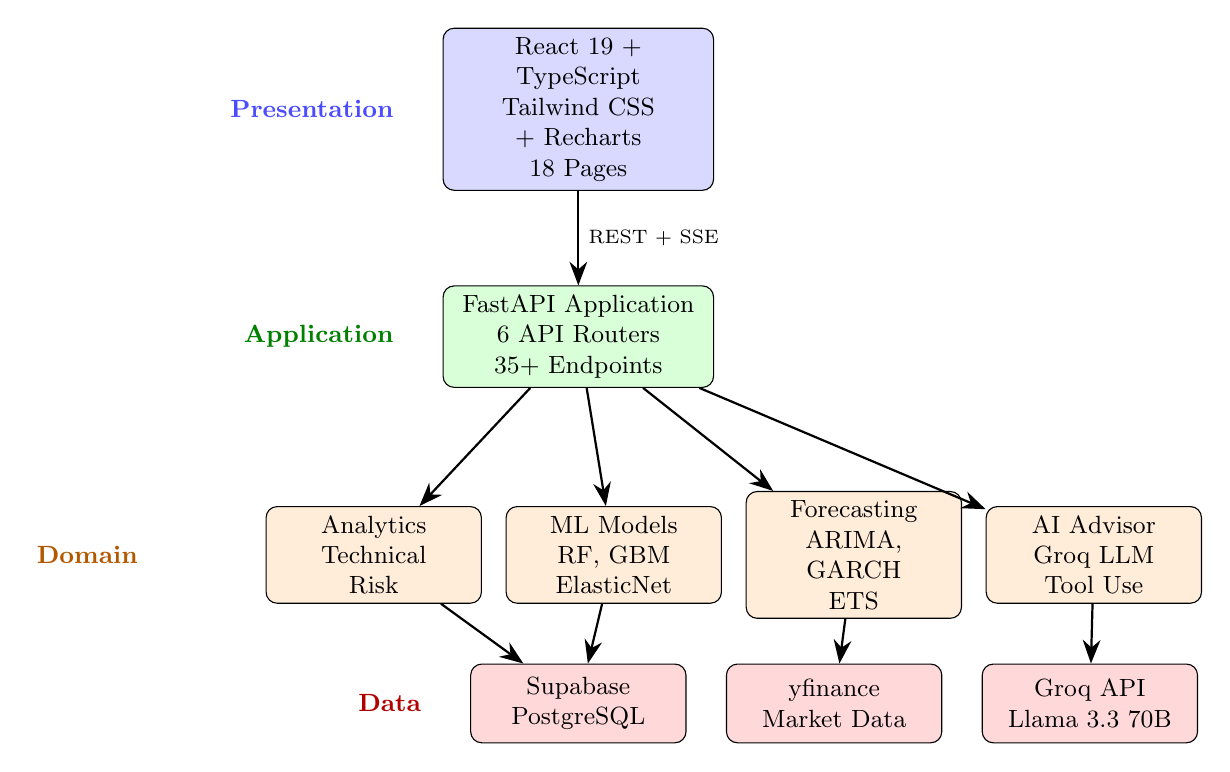
\begin{tikzpicture}[
    node distance=1.2cm,
    block/.style={rectangle, draw, rounded corners, text width=3.2cm, minimum height=1cm, align=center, font=\small},
    layer/.style={rectangle, draw, dashed, rounded corners, inner sep=10pt, fill=#1},
    arrow/.style={-{Stealth[length=3mm]}, thick}
]

% Presentation Layer
\node[block, fill=blue!15] (frontend) {React 19 + TypeScript\\Tailwind CSS + Recharts\\18 Pages};

% Application Layer
\node[block, fill=green!15, below=of frontend] (fastapi) {FastAPI Application\\6 API Routers\\35+ Endpoints};

% Service Layer
\node[block, fill=orange!15, below left=1.5cm and -0.5cm of fastapi, text width=2.5cm] (analytics) {Analytics\\Technical\\Risk};
\node[block, fill=orange!15, right=0.3cm of analytics, text width=2.5cm] (ml) {ML Models\\RF, GBM\\ElasticNet};
\node[block, fill=orange!15, right=0.3cm of ml, text width=2.5cm] (forecast) {Forecasting\\ARIMA, GARCH\\ETS};
\node[block, fill=orange!15, right=0.3cm of forecast, text width=2.5cm] (ai) {AI Advisor\\Groq LLM\\Tool Use};

% Data Layer
\node[block, fill=red!15, below=3.5cm of fastapi, text width=2.5cm] (supabase) {Supabase\\PostgreSQL};
\node[block, fill=red!15, right=0.5cm of supabase, text width=2.5cm] (yfinance) {yfinance\\Market Data};
\node[block, fill=red!15, right=0.5cm of yfinance, text width=2.5cm] (groq) {Groq API\\Llama 3.3 70B};

% Arrows
\draw[arrow] (frontend) -- node[right, font=\scriptsize] {REST + SSE} (fastapi);
\draw[arrow] (fastapi) -- (analytics);
\draw[arrow] (fastapi) -- (ml);
\draw[arrow] (fastapi) -- (forecast);
\draw[arrow] (fastapi) -- (ai);
\draw[arrow] (analytics) -- (supabase);
\draw[arrow] (ml) -- (supabase);
\draw[arrow] (forecast) -- (yfinance);
\draw[arrow] (ai) -- (groq);

% Layer labels
\node[left=0.5cm of frontend, font=\small\bfseries, text=blue!70] {Presentation};
\node[left=0.5cm of fastapi, font=\small\bfseries, text=green!50!black] {Application};
\node[left=1.5cm of analytics, font=\small\bfseries, text=orange!70!black] {Domain};
\node[left=0.5cm of supabase, font=\small\bfseries, text=red!70!black] {Data};

\end{tikzpicture}
\caption{High-level system architecture of \projectname{}}
\label{fig:system_arch}
\end{figure}

\subsection{Component Architecture}

The backend is composed of 19 independent service modules, organized into the following categories:

\begin{table}[H]
\centering
\caption{Backend service module inventory}
\label{tab:service_modules}
\begin{tabularx}{\textwidth}{@{}l l X@{}}
\toprule
\textbf{Category} & \textbf{Module} & \textbf{Responsibility} \\
\midrule
\multirow{3}{*}{Core Analytics} & analytics.py & Orchestrator, technical signals, stock universe, shared DF cache \\
& technical.py & 7-indicator weighted composite signal computation \\
& risk.py & Sharpe, beta, VaR, drawdown, Isolation Forest anomalies \\
\midrule
\multirow{4}{*}{Machine Learning} & ml/classifier.py & Random Forest BUY/HOLD/SELL classification \\
& ml/clustering.py & K-Means (k=4) stock segmentation \\
& ml/model\_store.py & PKL serialization for model persistence \\
& ml\_regression.py & 3-model ensemble (RF, ElasticNet, GBM) return forecasting \\
\midrule
\multirow{2}{*}{Forecasting} & timeseries.py & ARIMA, Holt-Winters ETS, seasonal decomposition \\
& volatility.py & GARCH(1,1), volatility cones, regime classification \\
\midrule
\multirow{3}{*}{Factor/Sector} & risk\_factors.py & Fama-French 4-factor OLS decomposition \\
& sector\_rotation.py & Multi-horizon momentum, market phase \\
& macro.py & India VIX, USD/INR, Gold, Crude Oil, regime \\
\midrule
\multirow{3}{*}{AI \& NLP} & ai\_advisor.py & Groq LLM with function calling, SSE streaming \\
& ai\_portfolio.py & LLM-powered portfolio construction \\
& news\_sentiment.py & Google News RSS, keyword lexicon scoring \\
\midrule
\multirow{3}{*}{Portfolio} & portfolio.py & Holdings \& watchlist CRUD, P\&L tracking \\
& portfolio\_optimizer.py & Markowitz MVO, efficient frontier \\
& portfolio\_backtester.py & Strategy backtesting vs benchmark \\
\midrule
\multirow{2}{*}{Planning} & financial\_engine.py & SIP calculator, goal solver, asset allocation \\
& monte\_carlo.py & 1,000 simulations, percentile wealth trajectories \\
\midrule
Data Access & market\_data.py & Unified data source: cache $\to$ Supabase $\to$ yfinance \\
\bottomrule
\end{tabularx}
\end{table}

\subsection{Data Flow Architecture}

The system implements a \textbf{unidirectional data flow} pattern. Data originates from external sources (yfinance, Google News RSS), flows through ingestion, storage, computation, and caching layers, and is ultimately delivered to the frontend via REST/SSE endpoints.

\begin{figure}[H]
\centering
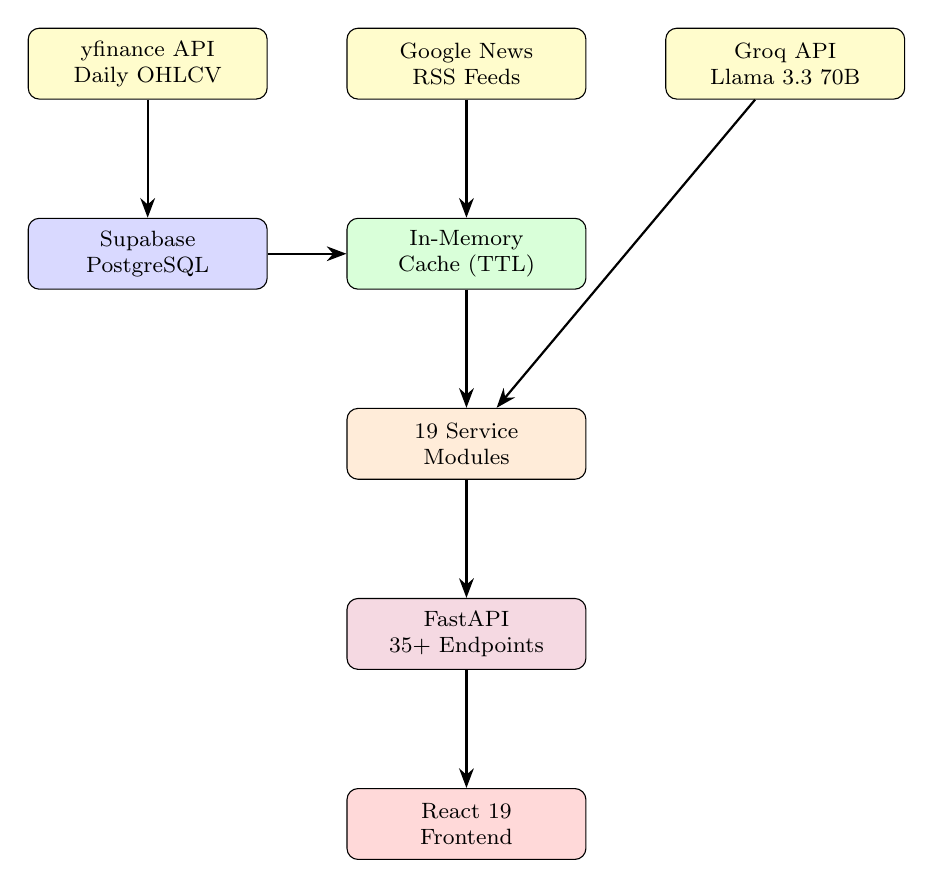
\begin{tikzpicture}[
    node distance=1.5cm,
    block/.style={rectangle, draw, rounded corners, text width=2.8cm, minimum height=0.9cm, align=center, font=\footnotesize},
    arrow/.style={-{Stealth[length=2.5mm]}, thick}
]

% Row 1: External Sources
\node[block, fill=yellow!20] (yf) {yfinance API\\Daily OHLCV};
\node[block, fill=yellow!20, right=1cm of yf] (news) {Google News\\RSS Feeds};
\node[block, fill=yellow!20, right=1cm of news] (groq) {Groq API\\Llama 3.3 70B};

% Row 2: Storage & Cache
\node[block, fill=blue!15, below=of yf] (db) {Supabase\\PostgreSQL};
\node[block, fill=green!15, below=of news] (cache) {In-Memory\\Cache (TTL)};

% Row 3: Computation
\node[block, fill=orange!15, below=of cache] (compute) {19 Service\\Modules};

% Row 4: API
\node[block, fill=purple!15, below=of compute] (api) {FastAPI\\35+ Endpoints};

% Row 5: Frontend
\node[block, fill=red!15, below=of api] (fe) {React 19\\Frontend};

% Arrows
\draw[arrow] (yf) -- (db);
\draw[arrow] (db) -- (cache);
\draw[arrow] (news) -- (cache);
\draw[arrow] (cache) -- (compute);
\draw[arrow] (groq) -- (compute);
\draw[arrow] (compute) -- (api);
\draw[arrow] (api) -- (fe);

\end{tikzpicture}
\caption{Data flow pipeline from external sources to frontend}
\label{fig:data_flow}
\end{figure}

\subsection{Deployment Architecture}

The production deployment spans three cloud platforms:

\begin{table}[H]
\centering
\caption{Deployment configuration}
\label{tab:deployment}
\begin{tabularx}{\textwidth}{@{}l l l X@{}}
\toprule
\textbf{Component} & \textbf{Platform} & \textbf{Protocol} & \textbf{Configuration} \\
\midrule
Frontend & Netlify CDN & HTTPS & SPA redirect, Vite build, auto-deploy \\
Backend & HF Spaces & HTTPS & Docker, Python 3.12, Uvicorn, port 7860 \\
Database & Supabase & PostgREST & Managed PostgreSQL, RLS enabled \\
LLM & Groq Cloud & HTTPS & OpenAI-compatible API, SSE streaming \\
\bottomrule
\end{tabularx}
\end{table}

\section{Database Design}
\label{sec:database_design}

\subsection{Entity-Relationship Model}

The database consists of six primary tables stored in Supabase (managed PostgreSQL):

\begin{figure}[H]
\centering
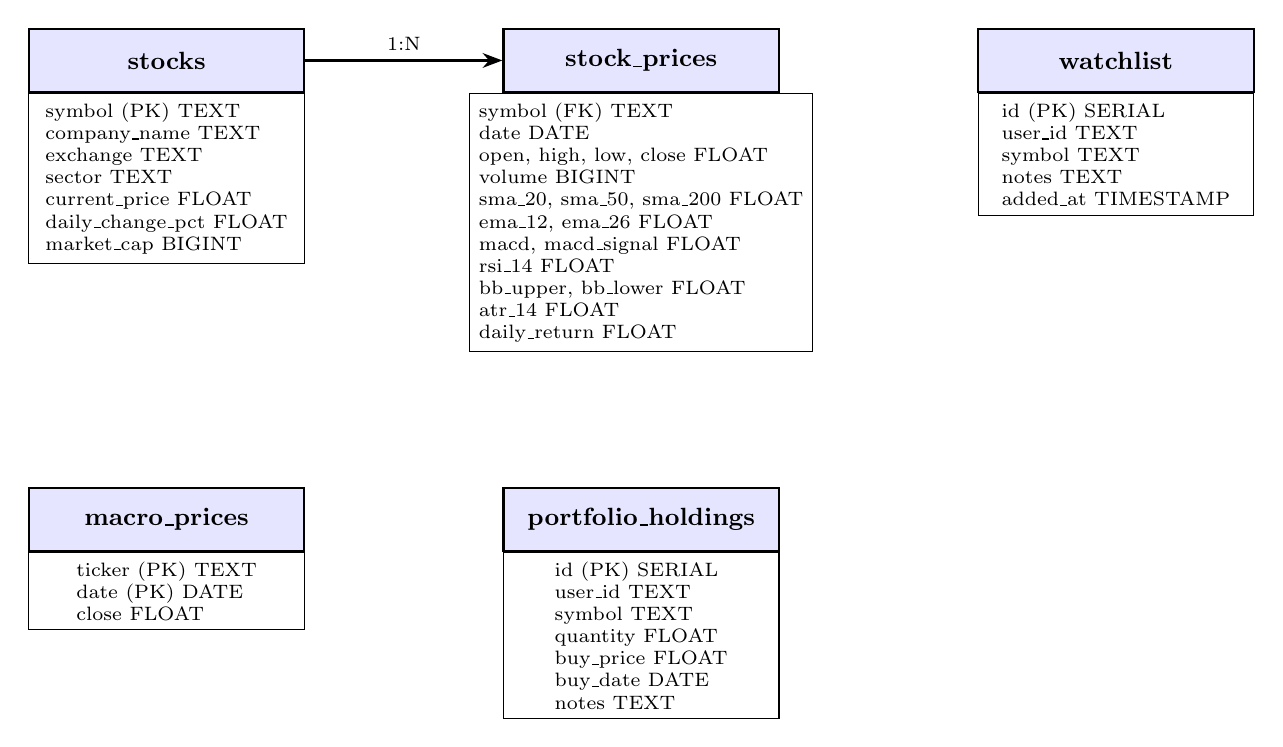
\begin{tikzpicture}[
    entity/.style={rectangle, draw, thick, fill=blue!10, minimum width=3.5cm, minimum height=0.8cm, font=\small\bfseries},
    attr/.style={rectangle, draw, fill=white, minimum width=3.5cm, font=\scriptsize, align=left},
    rel/.style={-{Stealth[length=2.5mm]}, thick}
]

% stocks table
\node[entity] (stocks) {stocks};
\node[attr, below=0pt of stocks] (stocks_attr) {
    symbol (PK) TEXT\\
    company\_name TEXT\\
    exchange TEXT\\
    sector TEXT\\
    current\_price FLOAT\\
    daily\_change\_pct FLOAT\\
    market\_cap BIGINT
};

% stock_prices table
\node[entity, right=2.5cm of stocks] (prices) {stock\_prices};
\node[attr, below=0pt of prices] (prices_attr) {
    symbol (FK) TEXT\\
    date DATE\\
    open, high, low, close FLOAT\\
    volume BIGINT\\
    sma\_20, sma\_50, sma\_200 FLOAT\\
    ema\_12, ema\_26 FLOAT\\
    macd, macd\_signal FLOAT\\
    rsi\_14 FLOAT\\
    bb\_upper, bb\_lower FLOAT\\
    atr\_14 FLOAT\\
    daily\_return FLOAT
};

% macro_prices table
\node[entity, below=5cm of stocks] (macro) {macro\_prices};
\node[attr, below=0pt of macro] (macro_attr) {
    ticker (PK) TEXT\\
    date (PK) DATE\\
    close FLOAT
};

% portfolio_holdings table
\node[entity, below=5cm of prices] (holdings) {portfolio\_holdings};
\node[attr, below=0pt of holdings] (holdings_attr) {
    id (PK) SERIAL\\
    user\_id TEXT\\
    symbol TEXT\\
    quantity FLOAT\\
    buy\_price FLOAT\\
    buy\_date DATE\\
    notes TEXT
};

% watchlist table
\node[entity, right=2.5cm of prices] (watchlist) {watchlist};
\node[attr, below=0pt of watchlist] (watchlist_attr) {
    id (PK) SERIAL\\
    user\_id TEXT\\
    symbol TEXT\\
    notes TEXT\\
    added\_at TIMESTAMP
};

% Relationships
\draw[rel] (stocks) -- node[above, font=\scriptsize] {1:N} (prices);

\end{tikzpicture}
\caption{Entity-Relationship diagram for the \projectname{} database}
\label{fig:er_diagram}
\end{figure}

\subsection{Indexing Strategy}

\begin{table}[H]
\centering
\caption{Database indexing strategy}
\label{tab:indexes}
\begin{tabularx}{\textwidth}{@{}l l X@{}}
\toprule
\textbf{Index} & \textbf{Table} & \textbf{Purpose} \\
\midrule
(symbol, date) UNIQUE & stock\_prices & Fast lookup + upsert deduplication \\
(symbol) & stock\_prices & Per-stock history queries \\
(date) & stock\_prices & Cross-stock date range queries \\
(ticker, date) UNIQUE & macro\_prices & Macro data deduplication \\
(sector) & stocks & Sector-based filtering \\
(user\_id) & portfolio\_holdings & User-specific portfolio queries \\
\bottomrule
\end{tabularx}
\end{table}

\section{API Design}
\label{sec:api_design}

The backend exposes 35+ RESTful endpoints organized into 6 routers under the \texttt{/api/v1/} prefix:

\begin{longtable}{@{}l l l p{6cm}@{}}
\toprule
\textbf{Router} & \textbf{Method} & \textbf{Endpoint} & \textbf{Description} \\
\midrule
\endhead
\multirow{2}{*}{Advisor} & POST & /chat & Non-streaming AI chat \\
& POST & /chat/stream & SSE streaming AI chat with tool use \\
\midrule
\multirow{10}{*}{Analytics} & GET & /report & Full ML analytics report \\
& GET & /market-overview & Sector heatmap, gainers, losers, anomalies \\
& GET & /stock-signals & Technical signals for all stocks \\
& GET & /stock/\{symbol\} & Full analysis for single stock \\
& GET & /screener & Multi-criteria stock screener \\
& POST & /portfolio-optimize & Efficient frontier optimization \\
& GET & /correlation & Pearson correlation matrix \\
& GET & /backtest/\{symbol\} & Strategy backtest vs benchmark \\
& GET & /timeseries/\{symbol\} & ARIMA/ETS time-series analysis \\
& GET & /model-health & MLOps model health dashboard \\
\midrule
\multirow{5}{*}{Advanced} & GET & /sector-rotation & Sector momentum rankings \\
& GET & /volatility/\{symbol\} & GARCH volatility forecast \\
& GET & /macro & Macro indicators and regime \\
& POST & /risk-factors & Fama-French factor decomposition \\
& GET & /ml-prediction/\{symbol\} & Multi-model ML prediction \\
\midrule
\multirow{7}{*}{Portfolio} & GET & /holdings & Get portfolio holdings \\
& POST & /holdings & Add holding \\
& DELETE & /holdings/\{id\} & Remove holding \\
& GET & /watchlist & Get watchlist \\
& POST & /watchlist & Add to watchlist \\
& DELETE & /watchlist/\{id\} & Remove from watchlist \\
& POST & /ai-build & AI portfolio builder \\
\midrule
\multirow{4}{*}{Stocks} & GET & /search & Search stocks by name/symbol \\
& GET & /\{symbol\}/history & Historical OHLCV data \\
& GET & /indices/summary & Market indices (Nifty, Sensex) \\
& GET & /sectors/performance & Sector-wise performance \\
\midrule
\multirow{2}{*}{Planner} & POST & /forward & Monte Carlo wealth projection \\
& POST & /goal & Goal-based SIP solver \\
\bottomrule
\caption{Complete API endpoint reference}
\label{tab:api_endpoints}
\end{longtable}

\section{Caching Architecture}
\label{sec:caching}

A multi-tier in-memory caching system minimizes latency and external API load. The \texttt{CacheManager} singleton implements TTL-based key-value storage with thread-safe operations:

\begin{table}[H]
\centering
\caption{Cache TTL configuration by data type}
\label{tab:cache_ttl}
\begin{tabularx}{\textwidth}{@{}l l X@{}}
\toprule
\textbf{Cache Key Pattern} & \textbf{TTL} & \textbf{Rationale} \\
\midrule
stock:df:\{symbol\} & 24 hours & Price data changes only after market close \\
analytics:report & 2 hours & Full ML pipeline is computationally expensive \\
ml:rf:\{symbol\} & 24 hours & Classifier retrained daily \\
ml:regression:\{symbol\} & 1 hour & Regression models evolve with new data \\
vol:\{symbol\} & 1 hour & Volatility shifts faster than price trends \\
sector:rotation & 1 hour & Momentum scores recalculated periodically \\
macro:dashboard & 30 minutes & Macro indicators are intraday-sensitive \\
news:sentiment & 30 minutes & News headlines change frequently \\
indices:summary & 5 minutes & Index values need near-real-time freshness \\
\bottomrule
\end{tabularx}
\end{table}

\section{UML Diagrams}
\label{sec:uml}

\subsection{Use Case Diagram}

\begin{figure}[H]
\centering
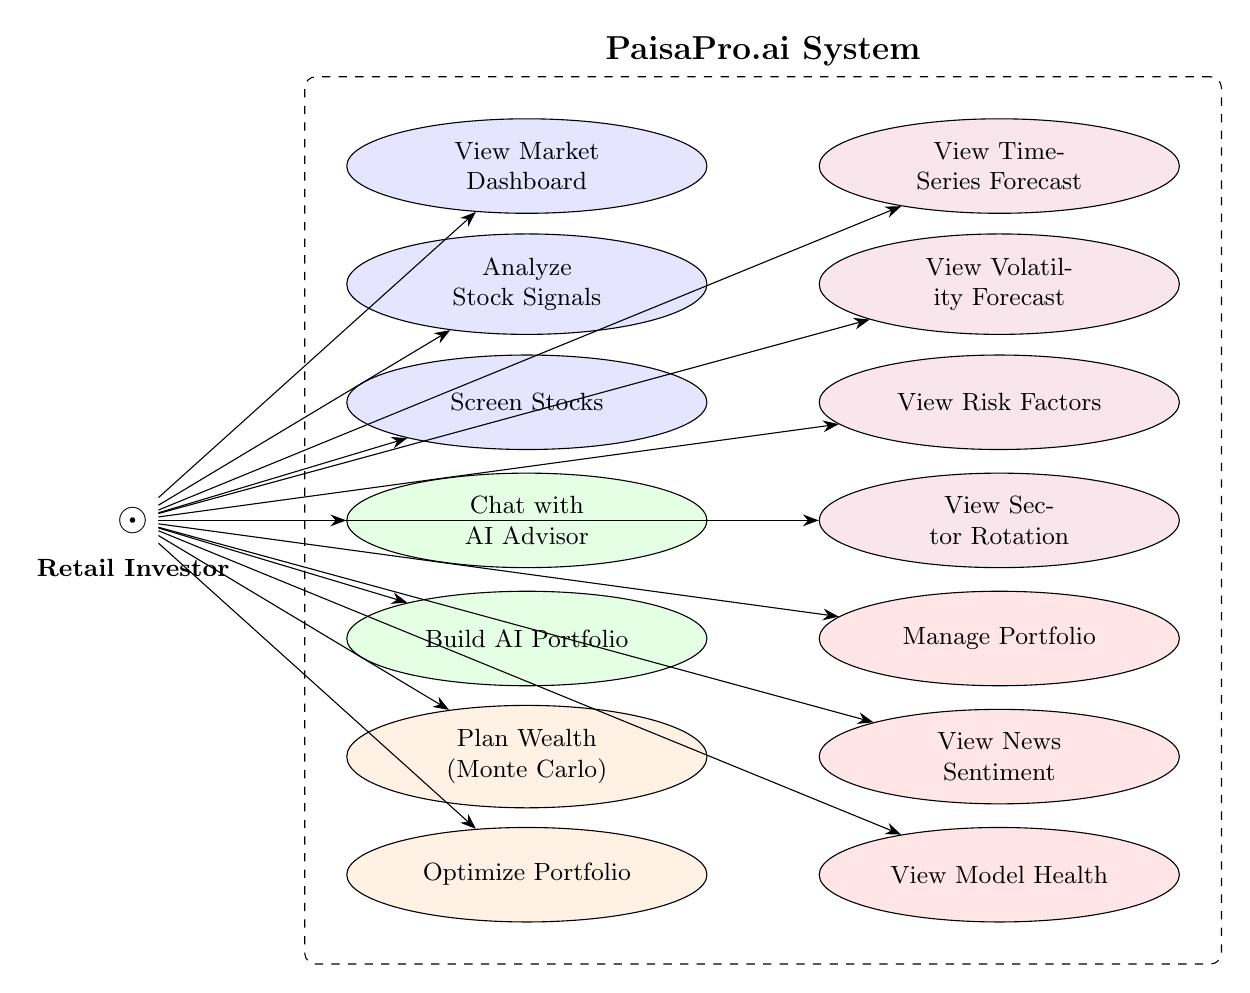
\begin{tikzpicture}[
    actor/.style={},
    usecase/.style={ellipse, draw, text width=3cm, align=center, font=\small, minimum height=1.2cm},
    arrow/.style={-{Stealth[length=2mm]}}
]

% Actor
\node[font=\Large] (user) at (0, 0) {\textbf{$\odot$}};
\node[below=2pt of user, font=\small\bfseries] {Retail Investor};

% Use cases - left column
\node[usecase, fill=blue!10] (uc1) at (5, 4.5) {View Market Dashboard};
\node[usecase, fill=blue!10] (uc2) at (5, 3) {Analyze Stock Signals};
\node[usecase, fill=blue!10] (uc3) at (5, 1.5) {Screen Stocks};
\node[usecase, fill=green!10] (uc4) at (5, 0) {Chat with AI Advisor};
\node[usecase, fill=green!10] (uc5) at (5, -1.5) {Build AI Portfolio};
\node[usecase, fill=orange!10] (uc6) at (5, -3) {Plan Wealth (Monte Carlo)};
\node[usecase, fill=orange!10] (uc7) at (5, -4.5) {Optimize Portfolio};

% Right column
\node[usecase, fill=purple!10] (uc8) at (11, 4.5) {View Time-Series Forecast};
\node[usecase, fill=purple!10] (uc9) at (11, 3) {View Volatility Forecast};
\node[usecase, fill=purple!10] (uc10) at (11, 1.5) {View Risk Factors};
\node[usecase, fill=purple!10] (uc11) at (11, 0) {View Sector Rotation};
\node[usecase, fill=red!10] (uc12) at (11, -1.5) {Manage Portfolio};
\node[usecase, fill=red!10] (uc13) at (11, -3) {View News Sentiment};
\node[usecase, fill=red!10] (uc14) at (11, -4.5) {View Model Health};

% Arrows
\foreach \i in {1,...,7} {
    \draw[arrow] (user) -- (uc\i);
}
\foreach \i in {8,...,14} {
    \draw[arrow] (user) -- (uc\i);
}

% System boundary
\node[draw, dashed, rounded corners, fit=(uc1)(uc2)(uc3)(uc4)(uc5)(uc6)(uc7)(uc8)(uc9)(uc10)(uc11)(uc12)(uc13)(uc14), inner sep=15pt, label={[font=\large\bfseries]above:\projectname{} System}] {};

\end{tikzpicture}
\caption{Use case diagram showing the 14 primary user interactions}
\label{fig:use_case}
\end{figure}

\subsection{Class Diagram (Backend Services)}

\begin{figure}[H]
\centering
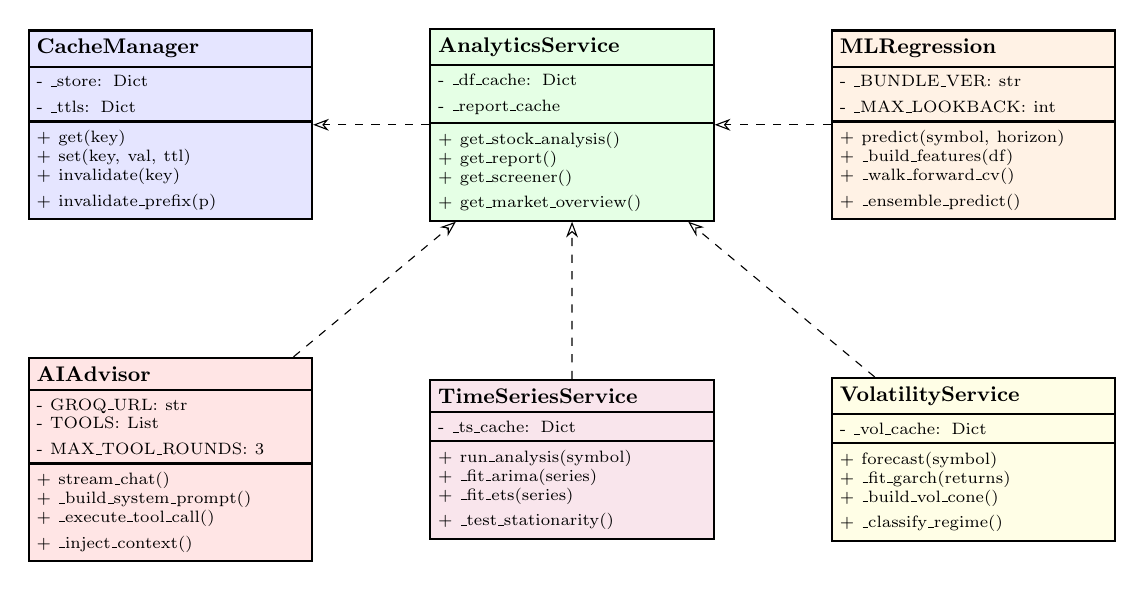
\begin{tikzpicture}[
    class/.style={rectangle split, rectangle split parts=3, draw, thick, text width=4cm, font=\small, fill=#1},
    dep/.style={-{Stealth[length=2mm, open]}, dashed},
    scale=0.85, transform shape
]

% CacheManager
\node[class=blue!10] (cache) at (0, 0) {
    \textbf{CacheManager}
    \nodepart{second}
    \scriptsize{- \_store: Dict}\\
    \scriptsize{- \_ttls: Dict}
    \nodepart{third}
    \scriptsize{+ get(key)}\\
    \scriptsize{+ set(key, val, ttl)}\\
    \scriptsize{+ invalidate(key)}\\
    \scriptsize{+ invalidate\_prefix(p)}
};

% AnalyticsService
\node[class=green!10] (analytics) at (6, 0) {
    \textbf{AnalyticsService}
    \nodepart{second}
    \scriptsize{- \_df\_cache: Dict}\\
    \scriptsize{- \_report\_cache}
    \nodepart{third}
    \scriptsize{+ get\_stock\_analysis()}\\
    \scriptsize{+ get\_report()}\\
    \scriptsize{+ get\_screener()}\\
    \scriptsize{+ get\_market\_overview()}
};

% MLRegression
\node[class=orange!10] (mlreg) at (12, 0) {
    \textbf{MLRegression}
    \nodepart{second}
    \scriptsize{- \_BUNDLE\_VER: str}\\
    \scriptsize{- \_MAX\_LOOKBACK: int}
    \nodepart{third}
    \scriptsize{+ predict(symbol, horizon)}\\
    \scriptsize{+ \_build\_features(df)}\\
    \scriptsize{+ \_walk\_forward\_cv()}\\
    \scriptsize{+ \_ensemble\_predict()}
};

% AIAdvisor
\node[class=red!10] (advisor) at (0, -5) {
    \textbf{AIAdvisor}
    \nodepart{second}
    \scriptsize{- GROQ\_URL: str}\\
    \scriptsize{- TOOLS: List}\\
    \scriptsize{- MAX\_TOOL\_ROUNDS: 3}
    \nodepart{third}
    \scriptsize{+ stream\_chat()}\\
    \scriptsize{+ \_build\_system\_prompt()}\\
    \scriptsize{+ \_execute\_tool\_call()}\\
    \scriptsize{+ \_inject\_context()}
};

% TimeSeries
\node[class=purple!10] (ts) at (6, -5) {
    \textbf{TimeSeriesService}
    \nodepart{second}
    \scriptsize{- \_ts\_cache: Dict}
    \nodepart{third}
    \scriptsize{+ run\_analysis(symbol)}\\
    \scriptsize{+ \_fit\_arima(series)}\\
    \scriptsize{+ \_fit\_ets(series)}\\
    \scriptsize{+ \_test\_stationarity()}
};

% Volatility
\node[class=yellow!10] (vol) at (12, -5) {
    \textbf{VolatilityService}
    \nodepart{second}
    \scriptsize{- \_vol\_cache: Dict}
    \nodepart{third}
    \scriptsize{+ forecast(symbol)}\\
    \scriptsize{+ \_fit\_garch(returns)}\\
    \scriptsize{+ \_build\_vol\_cone()}\\
    \scriptsize{+ \_classify\_regime()}
};

% Dependencies
\draw[dep] (analytics) -- (cache);
\draw[dep] (mlreg) -- (analytics);
\draw[dep] (advisor) -- (analytics);
\draw[dep] (ts) -- (analytics);
\draw[dep] (vol) -- (analytics);

\end{tikzpicture}
\caption{Simplified class diagram showing key backend services and their dependencies}
\label{fig:class_diagram}
\end{figure}

\subsection{Sequence Diagram: AI Advisor Chat Flow}

\begin{figure}[H]
\centering
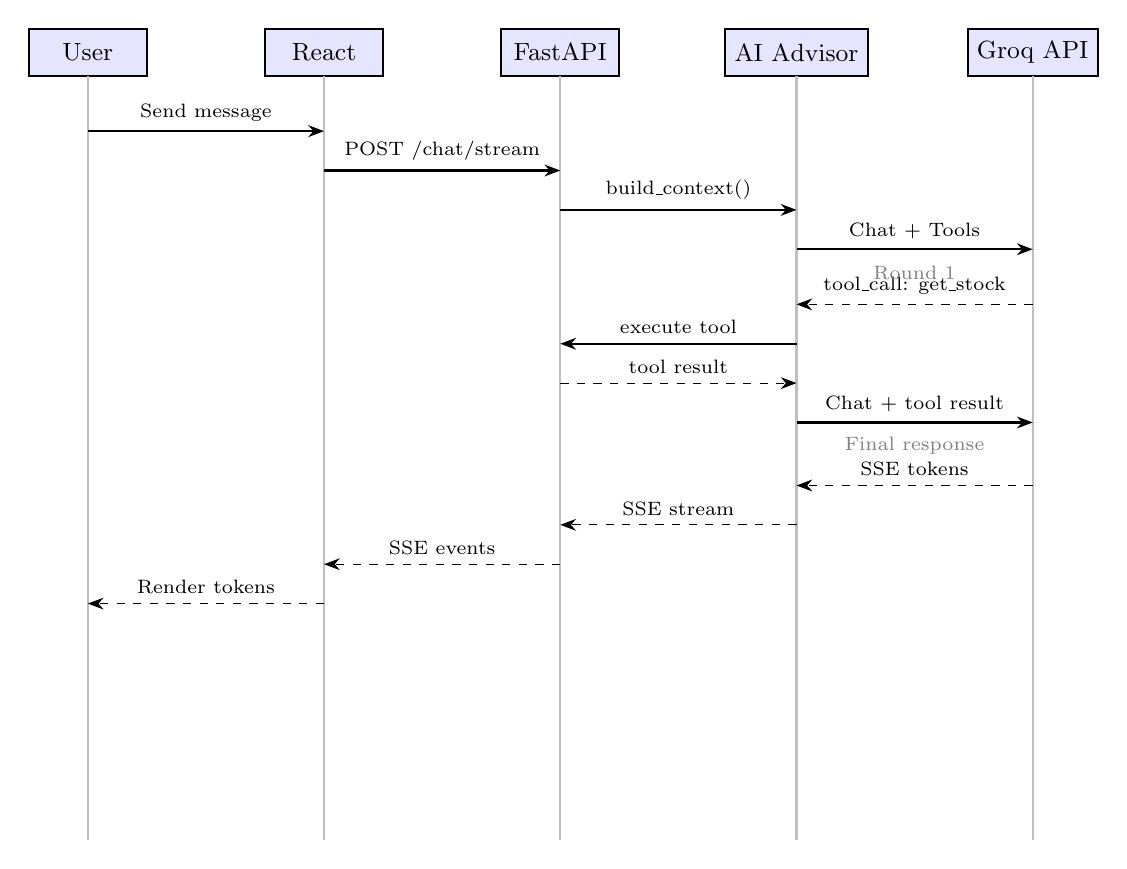
\begin{tikzpicture}[
    font=\small,
    lifeline/.style={thick},
    msg/.style={-{Stealth[length=2mm]}, thick},
    ret/.style={-{Stealth[length=2mm]}, dashed},
    actor/.style={rectangle, draw, thick, fill=blue!10, minimum width=1.5cm, minimum height=0.6cm, align=center}
]

% Actors
\node[actor] (user) at (0, 0) {User};
\node[actor] (fe) at (3, 0) {React};
\node[actor] (api) at (6, 0) {FastAPI};
\node[actor] (adv) at (9, 0) {AI Advisor};
\node[actor] (groq) at (12, 0) {Groq API};

% Lifelines
\foreach \x in {0, 3, 6, 9, 12} {
    \draw[lifeline, gray!50] (\x, -0.3) -- (\x, -10);
}

% Messages
\draw[msg] (0, -1) -- node[above, font=\scriptsize] {Send message} (3, -1);
\draw[msg] (3, -1.5) -- node[above, font=\scriptsize] {POST /chat/stream} (6, -1.5);
\draw[msg] (6, -2) -- node[above, font=\scriptsize] {build\_context()} (9, -2);
\draw[msg] (9, -2.5) -- node[above, font=\scriptsize] {Chat + Tools} (12, -2.5);
\draw[ret] (12, -3.2) -- node[above, font=\scriptsize] {tool\_call: get\_stock} (9, -3.2);
\draw[msg] (9, -3.7) -- node[above, font=\scriptsize] {execute tool} (6, -3.7);
\draw[ret] (6, -4.2) -- node[above, font=\scriptsize] {tool result} (9, -4.2);
\draw[msg] (9, -4.7) -- node[above, font=\scriptsize] {Chat + tool result} (12, -4.7);
\draw[ret] (12, -5.5) -- node[above, font=\scriptsize] {SSE tokens} (9, -5.5);
\draw[ret] (9, -6) -- node[above, font=\scriptsize] {SSE stream} (6, -6);
\draw[ret] (6, -6.5) -- node[above, font=\scriptsize] {SSE events} (3, -6.5);
\draw[ret] (3, -7) -- node[above, font=\scriptsize] {Render tokens} (0, -7);

% Annotations
\node[font=\scriptsize, text=gray] at (10.5, -2.8) {Round 1};
\node[font=\scriptsize, text=gray] at (10.5, -5) {Final response};

\end{tikzpicture}
\caption{Sequence diagram for AI advisor chat with tool-use loop}
\label{fig:sequence_advisor}
\end{figure}

\subsection{Activity Diagram: Daily Data Refresh Pipeline}

\begin{figure}[H]
\centering
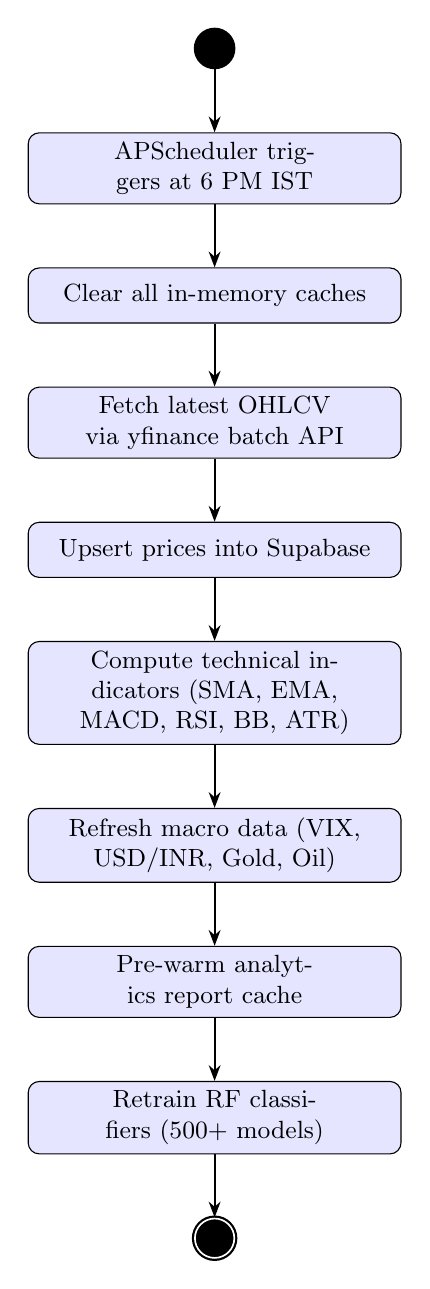
\begin{tikzpicture}[
    node distance=0.8cm,
    start/.style={circle, draw, thick, fill=black, minimum size=0.5cm},
    stop/.style={circle, draw, thick, fill=black, minimum size=0.5cm, double},
    action/.style={rectangle, draw, rounded corners, fill=blue!10, text width=4.5cm, minimum height=0.7cm, align=center, font=\small},
    decision/.style={diamond, draw, fill=yellow!20, aspect=2.5, font=\small},
    arrow/.style={-{Stealth[length=2mm]}, thick}
]

\node[start] (start) {};
\node[action, below=of start] (trigger) {APScheduler triggers at 6 PM IST};
\node[action, below=of trigger] (clear) {Clear all in-memory caches};
\node[action, below=of clear] (fetch) {Fetch latest OHLCV via yfinance batch API};
\node[action, below=of fetch] (upsert) {Upsert prices into Supabase};
\node[action, below=of upsert] (indicators) {Compute technical indicators (SMA, EMA, MACD, RSI, BB, ATR)};
\node[action, below=of indicators] (macro) {Refresh macro data (VIX, USD/INR, Gold, Oil)};
\node[action, below=of macro] (prewarm) {Pre-warm analytics report cache};
\node[action, below=of prewarm] (train) {Retrain RF classifiers (500+ models)};
\node[stop, below=of train] (stop) {};

% Arrows
\draw[arrow] (start) -- (trigger);
\draw[arrow] (trigger) -- (clear);
\draw[arrow] (clear) -- (fetch);
\draw[arrow] (fetch) -- (upsert);
\draw[arrow] (upsert) -- (indicators);
\draw[arrow] (indicators) -- (macro);
\draw[arrow] (macro) -- (prewarm);
\draw[arrow] (prewarm) -- (train);
\draw[arrow] (train) -- (stop);

\end{tikzpicture}
\caption{Activity diagram for the daily data refresh pipeline}
\label{fig:activity_refresh}
\end{figure}


% ########################################################################
%                     CHAPTER 4: METHODOLOGY
% ########################################################################
\chapter{Methodology}
\label{chap:methodology}

This chapter details the mathematical foundations, algorithms, and computational methods implemented in each analytical module of \projectname{}.

\section{Technical Indicator Computation}
\label{sec:meth_technical}

All technical indicators are computed from daily OHLCV data using lookback windows appropriate to each indicator.

\subsection{Simple Moving Average (SMA)}

The Simple Moving Average of period $n$ is defined as:
\begin{equation}
    SMA_n(t) = \frac{1}{n} \sum_{i=0}^{n-1} C_{t-i}
\end{equation}
where $C_t$ denotes the closing price at time $t$. Periods of 20 (short-term trend), 50 (medium-term), and 200 (long-term) are computed. Crossovers between SMA-50 and SMA-200 generate \textit{golden cross} (bullish) and \textit{death cross} (bearish) signals.

\subsection{Exponential Moving Average (EMA)}

The EMA applies exponentially decaying weights to past observations:
\begin{equation}
    EMA_n(t) = \alpha \cdot C_t + (1 - \alpha) \cdot EMA_n(t-1), \quad \alpha = \frac{2}{n+1}
\end{equation}
Periods of 12 and 26 are computed as inputs to the MACD calculation.

\subsection{MACD (Moving Average Convergence Divergence)}

\begin{align}
    MACD(t) &= EMA_{12}(t) - EMA_{26}(t) \\
    Signal(t) &= EMA_9\big(MACD(t)\big) \\
    Histogram(t) &= MACD(t) - Signal(t)
\end{align}

\textbf{Signal Logic:} MACD above signal line $\to$ bullish (+1); below $\to$ bearish ($-1$). Histogram divergence indicates momentum acceleration.

\subsection{RSI (Relative Strength Index)}

\begin{equation}
    RSI(t) = 100 - \frac{100}{1 + RS(t)}, \quad RS(t) = \frac{\overline{Gain}_{14}(t)}{\overline{Loss}_{14}(t)}
\end{equation}

\textbf{Signal Logic:} $RSI < 30 \to$ oversold (BUY, $+2$); $RSI > 70 \to$ overbought (SELL, $-2$); otherwise HOLD (0).

\subsection{Bollinger Bands}

\begin{align}
    \text{Upper Band}(t) &= SMA_{20}(t) + 2 \cdot \sigma_{20}(t) \\
    \text{Lower Band}(t) &= SMA_{20}(t) - 2 \cdot \sigma_{20}(t) \\
    \text{Width}(t) &= \frac{\text{Upper}(t) - \text{Lower}(t)}{SMA_{20}(t)}
\end{align}

\textbf{Signal Logic:} Price below lower band $\to$ oversold (BUY); above upper band $\to$ overbought (SELL). Band squeeze (narrowing width) indicates impending volatility expansion.

\subsection{ATR (Average True Range)}

\begin{equation}
    TR(t) = \max\big(H_t - L_t,\; |H_t - C_{t-1}|,\; |L_t - C_{t-1}|\big)
\end{equation}
\begin{equation}
    ATR_{14}(t) = \frac{1}{14} \sum_{i=0}^{13} TR(t-i)
\end{equation}

High ATR relative to price indicates elevated volatility; low ATR indicates consolidation.

\subsection{VWAP (Volume-Weighted Average Price)}

\begin{equation}
    VWAP = \frac{\sum_{i=1}^{N} (Price_i \times Volume_i)}{\sum_{i=1}^{N} Volume_i}
\end{equation}

Price above VWAP suggests bullish intraday bias; below suggests bearish.

\subsection{OBV (On-Balance Volume)}

\begin{equation}
    OBV(t) = OBV(t-1) + \begin{cases} V_t & \text{if } C_t > C_{t-1} \\ -V_t & \text{if } C_t < C_{t-1} \\ 0 & \text{otherwise} \end{cases}
\end{equation}

Rising OBV with rising price confirms trend strength through buying pressure.

\subsection{Composite Signal Generation}

Individual indicator signals are combined using a weighted ensemble:

\begin{table}[H]
\centering
\caption{Composite signal weights and mapping}
\label{tab:signal_weights}
\begin{tabular}{@{}lll@{}}
\toprule
\textbf{Indicator} & \textbf{Weight} & \textbf{Signal Mapping} \\
\midrule
RSI & 25\% & $<30 \to +2$, $>70 \to -2$, else $0$ \\
MACD & 20\% & Above signal $\to +1.5$, below $\to -1.5$ \\
Bollinger Bands & 20\% & Below lower $\to +1.5$, above upper $\to -1.5$ \\
ATR & 15\% & Low relative ATR $\to +1$, high $\to -1$ \\
ADX & 10\% & $>25$ with $+DI > -DI \to +1$, else $-1$ \\
VWAP & 5\% & Price $> VWAP \to +1$, $< VWAP \to -1$ \\
OBV & 5\% & Rising $\to +1$, falling $\to -1$ \\
\bottomrule
\end{tabular}
\end{table}

The composite score is computed as:
\begin{equation}
    Score = \sum_{i=1}^{7} w_i \cdot s_i
\end{equation}

\textbf{Classification:}
\begin{itemize}[nosep]
    \item $Score > +0.3 \to$ BUY
    \item $Score < -0.3 \to$ SELL
    \item Otherwise $\to$ HOLD
\end{itemize}

\textbf{Confidence:} Percentage of indicators agreeing with the composite direction (0--100\%).

\section{Machine Learning Models}
\label{sec:meth_ml}

\subsection{Random Forest Classifier --- Directional Prediction}

\textbf{Objective:} Predict whether a stock's price will be higher or lower in 5 trading days.

\textbf{Feature Set:}
\begin{table}[H]
\centering
\caption{Random Forest classifier features}
\label{tab:rf_features}
\begin{tabular}{@{}ll@{}}
\toprule
\textbf{Feature} & \textbf{Description} \\
\midrule
rsi\_14 & 14-day Relative Strength Index \\
macd & MACD line value \\
bb\_width & Bollinger Band width (normalized) \\
vol\_ratio & Volume / 20-day volume SMA \\
price\_vs\_sma20 & (Price $-$ SMA20) / SMA20 \\
daily\_return & Most recent daily return \\
\bottomrule
\end{tabular}
\end{table}

\textbf{Target:} Binary classification --- 1 if price 5 days ahead exceeds current price, else 0.

\textbf{Training Configuration:}
\begin{itemize}[nosep]
    \item Training window: 252 trading days (1 year)
    \item Estimators: 100 decision trees
    \item Train/test split: 80/20
    \item Minimum data requirement: 40 rows per stock
\end{itemize}

\textbf{Signal Mapping:}
\begin{itemize}[nosep]
    \item Probability $> 0.55 \to$ BUY
    \item Probability $\in [0.45, 0.55] \to$ HOLD
    \item Probability $< 0.45 \to$ SELL
\end{itemize}

\textbf{Model Persistence:} Trained models are serialized to pickle files with daily timestamps (\texttt{rf\_\{SYMBOL\}\_\{YYYYMMDD\}.pkl}). On each request, the system checks: (1) in-memory cache, (2) today's PKL on disk, (3) train from scratch.

\subsection{ML Regression Ensemble --- Return Forecasting}

\textbf{Objective:} Forecast $n$-day forward log-returns using three independent regression models.

\subsubsection{Feature Engineering}

The feature set is organized into three groups:

\textbf{(a) OHLC Microstructure Features (10 features):}
\begin{table}[H]
\centering
\caption{OHLC microstructure features}
\label{tab:ohlc_features}
\begin{tabular}{@{}ll@{}}
\toprule
\textbf{Feature} & \textbf{Formula / Description} \\
\midrule
hl\_pct & $(H - L) / C$ --- intraday range as \% of close \\
oc\_ret & $(C - O) / O$ --- intraday return \\
body\_pct & $|C - O| / (H - L)$ --- candle body strength \\
upper\_wick & $(H - \max(O,C)) / (H - L)$ --- upper wick proportion \\
lower\_wick & $(\min(O,C) - L) / (H - L)$ --- lower wick proportion \\
gap & $(O_t - C_{t-1}) / C_{t-1}$ --- overnight gap \\
dist\_52w\_high & Distance from 52-week high \\
dist\_52w\_low & Distance from 52-week low \\
williams\_r\_14 & Williams \%R overbought/oversold \\
channel\_pos\_20 & Position within 20-day Donchian channel \\
\bottomrule
\end{tabular}
\end{table}

\textbf{(b) Base Technical Features (10 features):} RSI-14, MACD, MACD signal, BB width, volume ratio, price vs SMA20/50, 5d/20d returns, ATR normalized.

\textbf{(c) Extended Features (12 features):} RSI moving average, MACD histogram, 10d/60d returns, momentum acceleration, log-scaled volume, volume ratio spread, BB position, SMA spread, price vs SMA200, RSI rate of change, volume ratio MA5.

\subsubsection{Target Variable}

The target is the \textbf{vol-adjusted log-return}:
\begin{equation}
    y_t = \frac{\ln(C_{t+h} / C_t)}{\hat{\sigma}_{20}(t)}
\end{equation}
where $\hat{\sigma}_{20}(t)$ is the 20-day rolling realized volatility. This Sharpe-signal target normalizes returns by their local volatility, making the target more comparable across stocks and time periods.

\subsubsection{Three Models}

\begin{enumerate}[nosep]
    \item \textbf{Random Forest Regressor:} 200 trees, max\_depth=6, max\_features=$\sqrt{p}$, trained on OHLC + base features.
    \item \textbf{ElasticNet (Ridge + Lasso):} L1 ratio=0.5, $\alpha=1.0$, trained on all features with RobustScaler preprocessing and 1st/99th percentile winsorization.
    \item \textbf{HistGradientBoosting:} 100 estimators, learning rate=0.05, max\_depth=4, early stopping after 10 rounds, trained on OHLC + base features.
\end{enumerate}

\subsubsection{Walk-Forward Cross-Validation}

To prevent look-ahead bias, a \textbf{rolling-window walk-forward} validation scheme is used:

\begin{algorithm}[H]
\caption{Walk-Forward Cross-Validation with Embargo}
\label{alg:walkforward}
\begin{algorithmic}[1]
\REQUIRE Time series data $D = \{(x_t, y_t)\}_{t=1}^{T}$, lookback window $W$, embargo $E$
\STATE Initialize $folds \leftarrow []$
\FOR{$i = 1$ to $K$}
    \STATE $train\_end \leftarrow W + i \cdot step$
    \STATE $test\_start \leftarrow train\_end + E$ \COMMENT{Embargo gap prevents leakage}
    \STATE $test\_end \leftarrow test\_start + step$
    \STATE Train model on $D[train\_end - W : train\_end]$
    \STATE Evaluate on $D[test\_start : test\_end]$
    \STATE Record MAE, RMSE, $R^2$, directional accuracy
\ENDFOR
\RETURN Mean metrics across $K$ folds
\end{algorithmic}
\end{algorithm}

\subsubsection{Ensemble and Confidence Intervals}

The ensemble prediction is a \textbf{Sharpe-weighted average}:
\begin{equation}
    \hat{y}_{ensemble} = \frac{\sum_{m=1}^{3} SR_m \cdot \hat{y}_m}{\sum_{m=1}^{3} SR_m}
\end{equation}
where $SR_m$ is the annualized Sharpe ratio of model $m$'s predictions (treating predictions as a long/short trading strategy).

The 80\% confidence interval is computed from the Random Forest tree distribution:
\begin{equation}
    CI_{80\%} = \hat{y}_{RF} \pm 1.28 \cdot \sigma_{trees}
\end{equation}
where $\sigma_{trees}$ is the standard deviation across all 200 tree predictions.

\subsection{Isolation Forest --- Anomaly Detection}

\textbf{Objective:} Detect unusual price movements and volume spikes.

\textbf{Features:} Absolute daily return percentage, volume ratio (current vs 20-day average).

\textbf{Algorithm:} Recursive random partitioning of feature space. Anomalous points require fewer splits to isolate, resulting in shorter average path lengths.

\textbf{Supplementary Rules:}
\begin{itemize}[nosep]
    \item Price spike: $|z_{return}| > 2.5$ standard deviations
    \item Volume spike: $|z_{volume}| > 2.5$ standard deviations
    \item High severity: $|z| > 3.5$
\end{itemize}

\subsection{K-Means Clustering --- Stock Segmentation}

\textbf{Objective:} Group stocks into $k=4$ behaviorally similar clusters.

\textbf{Features:} Annualized volatility, 3-month momentum (cumulative return), beta vs Nifty 50.

\textbf{Preprocessing:} StandardScaler (zero mean, unit variance).

\textbf{Cluster Labels (assigned by volatility ordering):}
\begin{enumerate}[nosep]
    \item \textbf{DEFENSIVE:} Low volatility, low beta, modest momentum
    \item \textbf{VALUE:} Moderate volatility, near-market beta
    \item \textbf{MOMENTUM:} High recent returns, moderate-to-high volatility
    \item \textbf{HIGH\_VOLATILITY:} Highest volatility and beta
\end{enumerate}

\section{Time-Series Forecasting}
\label{sec:meth_timeseries}

\subsection{Stationarity Testing}

Before fitting ARIMA models, the series is tested for stationarity:

\begin{enumerate}[nosep]
    \item \textbf{ADF Test:} $H_0$: unit root present (non-stationary). If $p > 0.05$, apply differencing.
    \item \textbf{KPSS Test:} $H_0$: series is stationary. Used as counter-validation.
    \item \textbf{Auto-Differencing:} If ADF fails, apply first differencing ($d=1$). If still non-stationary, apply second differencing ($d=2$). Maximum $d=2$.
\end{enumerate}

\subsection{ARIMA Model}

The ARIMA($p,d,q$) model is:
\begin{equation}
    \phi(B)(1-B)^d X_t = \theta(B)\epsilon_t
\end{equation}
where $\phi(B) = 1 - \phi_1 B - \cdots - \phi_p B^p$ is the AR polynomial, $\theta(B) = 1 + \theta_1 B + \cdots + \theta_q B^q$ is the MA polynomial, and $B$ is the backshift operator.

\textbf{Parameter Selection:}
\begin{itemize}[nosep]
    \item Grid search: $p \in \{0,1,2,3\}$, $d \in \{0,1,2\}$, $q \in \{0,1,2,3\}$
    \item Selection criterion: AIC (Akaike Information Criterion) --- lower is better
    \item Library: \texttt{statsmodels.tsa.arima.model.ARIMA}
\end{itemize}

\textbf{Forecast:} 30 trading days with 95\% confidence intervals.

\textbf{AIC Grid Search Algorithm:}
The optimal $(p, d, q)$ parameters are selected by exhaustive grid search minimizing the Akaike Information Criterion:

\begin{equation}
    AIC = 2k - 2\ln(\hat{L})
\end{equation}

where $k$ is the number of estimated parameters and $\hat{L}$ is the maximized likelihood. The grid search evaluates all combinations of $p \in \{0,1,2,3\}$, $d \in \{0,1,2\}$, $q \in \{0,1,2,3\}$, producing up to 48 candidate models. Models that fail to converge (common for over-parameterized specifications) are silently skipped. The model with the lowest AIC is selected.

\textbf{Confidence Interval Construction:}
The 95\% confidence intervals for the $h$-step-ahead forecast are constructed using the forecast standard error:

\begin{equation}
    CI_{t+h} = \hat{X}_{t+h} \pm 1.96 \times \hat{\sigma}_{t+h}
\end{equation}

where $\hat{\sigma}_{t+h}$ increases with the forecast horizon, reflecting growing uncertainty. For ARIMA models, the forecast standard error is derived from the MA representation of the process.

\textbf{Model Diagnostics:}
After fitting, the model residuals are checked for:
\begin{itemize}[nosep]
    \item \textbf{Normality:} Shapiro-Wilk test on standardized residuals
    \item \textbf{Autocorrelation:} Ljung-Box test at lags 1, 5, 10 --- significant autocorrelation indicates model inadequacy
    \item \textbf{Heteroskedasticity:} If residuals exhibit ARCH effects, this motivates the use of GARCH modelling (Section~\ref{sec:meth_volatility})
\end{itemize}

\subsection{Holt-Winters Exponential Smoothing (ETS)}

The damped trend model:
\begin{equation}
    \hat{y}_{t+h} = l_t + \sum_{j=1}^{h} \phi^j \cdot b_t
\end{equation}
where $l_t$ is the level, $b_t$ is the trend, and $\phi \in (0,1)$ is the damping parameter.

\textbf{Configuration:} Additive trend with damping, no seasonal component (daily stock data), scipy minimize (MSE objective).

\subsection{Seasonal Decomposition}

Additive decomposition: $X_t = T_t + S_t + R_t$

Using STL (Seasonal and Trend decomposition using LOESS) with period = 5 trading days.

\section{Volatility Modelling}
\label{sec:meth_volatility}

\subsection{GARCH(1,1) Model}

\textbf{Mean Equation:}
\begin{equation}
    r_t = \mu + \epsilon_t, \quad \epsilon_t = \sigma_t z_t, \quad z_t \sim N(0,1)
\end{equation}

\textbf{Variance Equation:}
\begin{equation}
    \sigma_t^2 = \omega + \alpha \epsilon_{t-1}^2 + \beta \sigma_{t-1}^2
\end{equation}

\textbf{Constraints:} $\omega > 0$, $\alpha \geq 0$, $\beta \geq 0$, $\alpha + \beta < 1$ (stationarity).

\textbf{Input:} Daily log returns scaled by 100 for numerical stability.

\textbf{Long-Run Variance:}
The unconditional (long-run) variance implied by the GARCH(1,1) model is:
\begin{equation}
    \bar{\sigma}^2 = \frac{\omega}{1 - \alpha - \beta}
\end{equation}

This quantity represents the mean-reverting level of volatility. When current conditional variance $\sigma_t^2 > \bar{\sigma}^2$, the model predicts declining volatility; when $\sigma_t^2 < \bar{\sigma}^2$, it predicts increasing volatility. This mean-reversion property is the basis for the entry/exit signals generated by the system.

\textbf{Persistence:}
The persistence parameter $P = \alpha + \beta$ determines how quickly volatility shocks decay. For most NSE-listed stocks, $P \in [0.90, 0.99]$, indicating that volatility shocks are highly persistent. The half-life of a volatility shock is:
\begin{equation}
    t_{1/2} = \frac{\ln(0.5)}{\ln(\alpha + \beta)}
\end{equation}

For a stock with $P = 0.95$, the half-life is approximately 13.5 trading days.

\textbf{Annualized Volatility:}
\begin{equation}
    \sigma_{annual} = \hat{\sigma}_{daily} \times \sqrt{252}
\end{equation}

\textbf{Estimation:} Maximum Likelihood Estimation (MLE) using the \texttt{arch} Python library. The optimizer uses the BFGS algorithm with analytically computed gradients. Convergence is verified by checking that the Hessian matrix is positive definite at the solution.

\textbf{Forecast Horizon:} 30 trading days.

\subsection{Volatility Cone Construction}

Realized volatility is computed across lookback windows of 10, 21, 63, 126, and 252 days. For each window, the percentile distribution (min, 25th, 50th, 75th, max) of rolling realized volatility is computed, forming the ``cone.''

\subsection{Regime Classification}

\begin{table}[H]
\centering
\caption{Volatility regime classification thresholds}
\label{tab:vol_regimes}
\begin{tabular}{@{}ll@{}}
\toprule
\textbf{Regime} & \textbf{Condition} \\
\midrule
LOW & Volatility $<$ 25th percentile of 1-year history \\
NORMAL & 25th $\leq$ Volatility $<$ 75th percentile \\
HIGH & 75th $\leq$ Volatility $<$ 95th percentile \\
EXTREME & Volatility $\geq$ 95th percentile \\
\bottomrule
\end{tabular}
\end{table}

\subsection{Entry/Exit Signals}

\begin{itemize}[nosep]
    \item LOW regime $\to$ LOW\_VOL\_ENTRY (favorable entry conditions)
    \item HIGH/EXTREME regime $\to$ HIGH\_VOL\_CAUTION (elevated risk)
    \item NORMAL regime $\to$ NEUTRAL
\end{itemize}

\section{Risk Analytics}
\label{sec:meth_risk}

\subsection{Risk Metrics Suite}

For each stock, the following metrics are computed from 1-year daily return data:

\begin{table}[H]
\centering
\caption{Risk metrics with formulas}
\label{tab:risk_metrics}
\begin{tabularx}{\textwidth}{@{}l l X@{}}
\toprule
\textbf{Metric} & \textbf{Formula} & \textbf{Interpretation} \\
\midrule
Annualized Volatility & $\sigma_{daily} \times \sqrt{252}$ & Total risk \\
Sharpe Ratio & $(R_p - R_f) / \sigma_p$, $R_f = 6.5\%$ & Risk-adjusted return \\
Sortino Ratio & $(R_p - R_f) / \sigma_{downside}$ & Downside risk-adjusted return \\
Max Drawdown & $\max\left(\frac{Peak - Trough}{Peak}\right)$ & Worst peak-to-trough decline \\
VaR (95\%) & 5th percentile of daily returns & Max expected daily loss \\
Beta & $\frac{Cov(R_i, R_m)}{Var(R_m)}$ & Systematic risk vs Nifty 50 \\
Alpha (Jensen's) & $R_i - [R_f + \beta(R_m - R_f)]$ & Excess return vs CAPM \\
\bottomrule
\end{tabularx}
\end{table}

\subsection{Fama-French 4-Factor Model}

\begin{equation}
    R_i - R_f = \alpha + \beta_1(R_m - R_f) + \beta_2 \cdot SMB + \beta_3 \cdot HML + \beta_4 \cdot MOM + \epsilon
\end{equation}

\textbf{Factor Proxy Construction:}

\begin{table}[H]
\centering
\caption{Fama-French factor proxy construction}
\label{tab:ff_factors}
\begin{tabularx}{\textwidth}{@{}l X@{}}
\toprule
\textbf{Factor} & \textbf{Proxy Construction} \\
\midrule
Market ($R_m - R_f$) & Nifty 50 excess returns over 6.5\% risk-free rate \\
SMB (Size) & Return of small-cap minus large-cap stocks (price median split) \\
HML (Value) & Return of high-P/E minus low-P/E stocks (price tercile split) \\
MOM (Momentum) & Return of top-momentum minus bottom-momentum stocks (6-month) \\
\bottomrule
\end{tabularx}
\end{table}

\textbf{Estimation:} OLS regression over 252 trading days.

\textbf{Output:} Alpha (annualized), factor betas, t-statistics, p-values, $R^2$, residual volatility, dominant factor.

\section{Portfolio Optimization}
\label{sec:meth_portfolio}

\subsection{Markowitz Mean-Variance Optimization}

Given $n$ assets with expected return vector $\boldsymbol{\mu}$ and covariance matrix $\boldsymbol{\Sigma}$:

\begin{equation}
    \min_{\mathbf{w}} \quad \mathbf{w}^T \boldsymbol{\Sigma} \mathbf{w}
\end{equation}
\begin{equation}
    \text{s.t.} \quad \mathbf{w}^T \boldsymbol{\mu} = \mu_{target}, \quad \sum_{i=1}^{n} w_i = 1, \quad w_i \geq 0, \quad w_i \leq 0.4
\end{equation}

\textbf{Implementation:}
\begin{enumerate}[nosep]
    \item Compute expected returns: annualized mean of daily returns
    \item Compute covariance matrix: sample covariance $\times$ 252
    \item Generate 2,000 random portfolios (Dirichlet sampling)
    \item Optimize via \texttt{scipy.optimize.minimize} (SLSQP method)
    \item Identify: minimum variance portfolio, maximum Sharpe portfolio
\end{enumerate}

\subsection{Target Volatilities by Risk Profile}

\begin{table}[H]
\centering
\caption{Target portfolio volatility by risk profile}
\label{tab:target_vol}
\begin{tabular}{@{}ll@{}}
\toprule
\textbf{Risk Profile} & \textbf{Target Volatility} \\
\midrule
Conservative & 12\% \\
Moderate & 18\% \\
Aggressive & 25\% \\
\bottomrule
\end{tabular}
\end{table}

\section{Monte Carlo Wealth Projection}
\label{sec:meth_montecarlo}

\subsection{Forward Planner}

For each simulation $s = 1, \ldots, 1000$ and each month $t$:

\begin{equation}
    R_t^{(s)} \sim N\left(\frac{\mu}{12}, \frac{\sigma}{\sqrt{12}}\right)
\end{equation}
\begin{equation}
    W_t^{(s)} = W_{t-1}^{(s)} \times (1 + R_t^{(s)}) + SIP_t
\end{equation}

where $SIP_t$ increases annually by the step-up percentage.

\textbf{Return Assumptions by Risk Profile:}
\begin{table}[H]
\centering
\caption{Monte Carlo return assumptions}
\label{tab:mc_assumptions}
\begin{tabular}{@{}lll@{}}
\toprule
\textbf{Profile} & \textbf{Expected Return ($\mu$)} & \textbf{Std Dev ($\sigma$)} \\
\midrule
Conservative & 9\% & 4\% \\
Moderate & 12\% & 8\% \\
Aggressive & 15\% & 14\% \\
\bottomrule
\end{tabular}
\end{table}

\textbf{Output:} Percentile trajectories (P10, P25, P50, P75, P90), probability of loss, year-by-year statistics.

\subsection{Goal Planner (Reverse Solver)}

Given target wealth $W_{target}$ and horizon $T$, find the minimum monthly SIP such that the median (P50) outcome meets the target:

\begin{algorithm}[H]
\caption{Goal-Based SIP Solver via Binary Search}
\label{alg:goal_solver}
\begin{algorithmic}[1]
\REQUIRE Target $W_{target}$, horizon $T$ years, risk profile
\STATE $lo \leftarrow 0$, $hi \leftarrow W_{target} / (T \times 12)$
\WHILE{$hi - lo > 0.01 \times lo$}
    \STATE $mid \leftarrow (lo + hi) / 2$
    \STATE Run 1,000 Monte Carlo simulations with $SIP = mid$
    \STATE $median \leftarrow$ P50 of terminal wealth distribution
    \IF{$median \geq W_{target}$}
        \STATE $hi \leftarrow mid$
    \ELSE
        \STATE $lo \leftarrow mid$
    \ENDIF
\ENDWHILE
\RETURN $hi$
\end{algorithmic}
\end{algorithm}

\section{Sector Rotation Analysis}
\label{sec:meth_sector}

\subsection{Multi-Horizon Momentum}

Sector momentum is computed across four horizons with weighted aggregation:

\begin{equation}
    M_{sector} = 0.10 \cdot R_{1M} + 0.20 \cdot R_{3M} + 0.30 \cdot R_{6M} + 0.40 \cdot R_{12M}
\end{equation}

where $R_{nM}$ is the average return of constituent stocks over $n$ months.

\subsection{Market Phase Detection}

Market phase is determined by Nifty 50 returns:
\begin{table}[H]
\centering
\caption{Market phase classification}
\label{tab:market_phase}
\begin{tabular}{@{}ll@{}}
\toprule
\textbf{Phase} & \textbf{Condition} \\
\midrule
EXPANSION & 3M return $> 0$ AND 12M return $> 0$ \\
PEAK & 3M return $< 0$ AND 12M return $> 0$ \\
CONTRACTION & 3M return $< 0$ AND 12M return $< 0$ \\
TROUGH & 3M return $> 0$ AND 12M return $< 0$ \\
\bottomrule
\end{tabular}
\end{table}

\section{Macroeconomic Dashboard}
\label{sec:meth_macro}

\subsection{Tracked Indicators}

\begin{table}[H]
\centering
\caption{Macroeconomic indicators tracked}
\label{tab:macro_indicators}
\begin{tabularx}{\textwidth}{@{}l l X@{}}
\toprule
\textbf{Indicator} & \textbf{Ticker} & \textbf{Significance} \\
\midrule
Nifty 50 & \textasciicircum NSEI & Broad market benchmark \\
Bank Nifty & \textasciicircum NSEBANK & Financial sector health \\
India VIX & \textasciicircum INDIAVIX & Market fear gauge \\
USD/INR & INR=X & Currency risk, FII flow indicator \\
Gold & GC=F & Safe haven, inflation hedge \\
Crude Oil & CL=F & Input cost, current account impact \\
\bottomrule
\end{tabularx}
\end{table}

\subsection{Regime Classification}

\begin{itemize}[nosep]
    \item VIX falling + Nifty rising + INR stable/strengthening $\to$ \textbf{RISK\_ON}
    \item VIX rising + Nifty falling + INR weakening $\to$ \textbf{RISK\_OFF}
    \item Mixed signals $\to$ \textbf{NEUTRAL}
\end{itemize}

\section{News Sentiment Analysis}
\label{sec:meth_sentiment}

\textbf{Data Source:} Google News RSS feeds for 25+ major Indian stocks.

\textbf{Scoring Algorithm:}
\begin{enumerate}[nosep]
    \item Parse RSS XML to extract headlines
    \item For each headline, count positive keyword matches ($p$) and negative keyword matches ($n$)
    \item Compute sentiment score: $S = \frac{p - n}{p + n}$ (range: $[-1, +1]$)
    \item Classify: $S > 0.15 \to$ POSITIVE; $S < -0.15 \to$ NEGATIVE; else NEUTRAL
    \item Aggregate: mean sentiment per stock across recent articles
\end{enumerate}

The lexicon contains 40+ positive terms (surge, rally, gain, bullish, upgrade, outperform) and 40+ negative terms (crash, fall, plunge, bearish, downgrade, sell-off).

\section{AI Advisory System}
\label{sec:meth_ai}

\subsection{LLM Integration}

\begin{table}[H]
\centering
\caption{AI advisor configuration}
\label{tab:ai_config}
\begin{tabularx}{\textwidth}{@{}l X@{}}
\toprule
\textbf{Parameter} & \textbf{Value} \\
\midrule
Provider & Groq Cloud \\
Model & Llama 3.3 70B Versatile \\
Interface & OpenAI-compatible chat completions API \\
Temperature & 0.7 (chat), 0.3 (portfolio construction) \\
Streaming & Server-Sent Events (SSE) \\
Max conversation history & 30 messages \\
Max tool rounds & 3 (prevents infinite loops) \\
\bottomrule
\end{tabularx}
\end{table}

\subsection{Agentic Tool Use (Function Calling)}

The AI advisor has access to four live tools:

\begin{table}[H]
\centering
\caption{AI advisor tool definitions}
\label{tab:ai_tools}
\begin{tabularx}{\textwidth}{@{}l X@{}}
\toprule
\textbf{Tool} & \textbf{Description} \\
\midrule
get\_stock\_analysis & Returns technical signals, risk metrics, RF probability, anomalies for a stock \\
get\_macro\_dashboard & Returns current macro indicators and market regime \\
get\_news\_sentiment & Returns news sentiment scores for stocks \\
run\_screener & Filters stocks by signal, sector, Sharpe ratio, drawdown \\
\bottomrule
\end{tabularx}
\end{table}

\textbf{Tool-Use Loop:} When the LLM responds with a \texttt{tool\_calls} array, the system: (1) executes the requested function, (2) appends the result as a tool message, (3) sends the updated conversation back to the LLM. This loop continues for up to 3 rounds, enabling multi-step reasoning.

\subsection{Context Injection}

The system prompt is dynamically constructed with:
\begin{enumerate}[nosep]
    \item User financial profile (income, expenses, savings, risk profile, age)
    \item Current portfolio holdings (symbols, quantities, buy prices, P\&L)
    \item Watchlist items (symbols, current prices, daily changes)
    \item Market snapshot (top BUY/SELL signals, sector performance, anomalies)
\end{enumerate}

This context injection transforms the generic LLM into a personalized financial advisor with real-time market awareness.


% ########################################################################
%                   CHAPTER 5: IMPLEMENTATION
% ########################################################################
\chapter{Implementation}
\label{chap:implementation}

This chapter details the technology stack, project structure, key code implementations, and deployment configuration of \projectname{}.

\section{Technology Stack}
\label{sec:tech_stack}

\subsection{Backend Technologies}

\begin{table}[H]
\centering
\caption{Backend technology stack}
\label{tab:backend_stack}
\begin{tabularx}{\textwidth}{@{}l l X@{}}
\toprule
\textbf{Category} & \textbf{Technology} & \textbf{Purpose} \\
\midrule
Web Framework & FastAPI 0.111 & REST API with async support, auto-docs \\
Server & Uvicorn & ASGI server \\
Language & Python 3.12 & Backend logic \\
Validation & Pydantic v2 & Request/response schema validation \\
HTTP Client & httpx 0.27 & Async HTTP for Supabase \& Groq \\
Data Processing & pandas 2.2.2 & DataFrame operations \\
Numerical & numpy 1.26.4 & Array computations \\
ML Framework & scikit-learn 1.8 & RF, GBM, ElasticNet, IF, KMeans \\
Time-Series & statsmodels 0.14.6 & ARIMA, ETS, ADF/KPSS tests \\
Volatility & arch 8.0.0 & GARCH modelling \\
Optimization & scipy 1.17.1 & Portfolio optimization (SLSQP) \\
Scheduling & APScheduler 3.10 & Daily cron job \\
Market Data & yfinance 0.2.40 & NSE stock data \\
Configuration & python-dotenv & Environment variable management \\
\bottomrule
\end{tabularx}
\end{table}

\subsection{Frontend Technologies}

\begin{table}[H]
\centering
\caption{Frontend technology stack}
\label{tab:frontend_stack}
\begin{tabularx}{\textwidth}{@{}l l X@{}}
\toprule
\textbf{Category} & \textbf{Technology} & \textbf{Purpose} \\
\midrule
UI Library & React 19 & Component-based UI \\
Language & TypeScript 5.9 & Type-safe JavaScript \\
Build Tool & Vite 8.0 & Fast HMR dev server + production bundler \\
Styling & Tailwind CSS 4 & Utility-first CSS with dark/light theme \\
State (Client) & Zustand 5.0 & Persisted client state (profile, theme) \\
State (Server) & TanStack React Query 5 & Server state caching, refetching \\
Charts & Recharts 3.8 & Line, Bar, Area, Scatter, Pie, Radar charts \\
Routing & React Router 7.13 & SPA client-side routing \\
HTTP Client & Axios 1.13 & REST API calls \\
Icons & Lucide React 0.577 & SVG icon library \\
Markdown & react-markdown 10.1 & LLM response rendering \\
\bottomrule
\end{tabularx}
\end{table}

\subsection{Infrastructure}

\begin{table}[H]
\centering
\caption{Infrastructure and deployment stack}
\label{tab:infra_stack}
\begin{tabularx}{\textwidth}{@{}l l X@{}}
\toprule
\textbf{Component} & \textbf{Platform} & \textbf{Details} \\
\midrule
Database & Supabase Cloud & Managed PostgreSQL, PostgREST API \\
Frontend Hosting & Netlify CDN & Static SPA, auto-deploy \\
Backend Hosting & HF Spaces & Docker container, cpu-basic tier \\
LLM Provider & Groq Cloud & Llama 3.3 70B, streaming API \\
Containerization & Docker & Python 3.12-slim base image \\
\bottomrule
\end{tabularx}
\end{table}

\section{Development Methodology and Workflow}
\label{sec:dev_methodology}

The project followed an iterative, module-driven development methodology with the following phases:

\subsection{Phase 1: Foundation (Data Layer)}

The first phase established the data pipeline and storage infrastructure:
\begin{enumerate}[nosep]
    \item Set up Supabase cloud database with the required tables (stocks, prices, holdings, watchlist, macro indicators)
    \item Implemented the \texttt{stock\_repository.py} and \texttt{macro\_repository.py} data access layers
    \item Built the daily data refresh pipeline using yfinance for OHLCV data ingestion
    \item Implemented the \texttt{CacheManager} singleton with TTL-based expiry and prefix invalidation
\end{enumerate}

\subsection{Phase 2: Analytics Engine}

With reliable data access established, the analytical services were built incrementally:
\begin{enumerate}[nosep]
    \item \textbf{Technical Analysis:} Implemented 7 technical indicators and the composite signal engine
    \item \textbf{ML Classification:} Random Forest directional prediction with feature engineering
    \item \textbf{ML Regression:} Three-model ensemble with walk-forward cross-validation
    \item \textbf{Anomaly Detection:} Isolation Forest for unusual price/volume detection
    \item \textbf{K-Means Clustering:} Stock segmentation by risk-return characteristics
    \item \textbf{Time-Series:} ARIMA (AIC grid search) and Holt-Winters ETS forecasting
    \item \textbf{GARCH:} Volatility forecasting with regime classification
    \item \textbf{Fama-French:} 4-factor model with proxy factor construction
    \item \textbf{Portfolio Optimization:} Markowitz MVO with Monte Carlo and SLSQP
    \item \textbf{Monte Carlo:} Forward planner and goal-based reverse solver
    \item \textbf{Sector Rotation:} Multi-horizon momentum with market phase detection
    \item \textbf{News Sentiment:} RSS-based headline sentiment pipeline
\end{enumerate}

Each service module was developed as an independent Python class with clear interfaces, enabling parallel development and isolated testing. Services communicate through well-defined return types using Pydantic schemas.

\subsection{Phase 3: API Layer}

The REST API was designed following RESTful conventions with OpenAPI documentation:
\begin{enumerate}[nosep]
    \item Six FastAPI routers organized by domain (advisor, analytics, advanced analytics, portfolio, stocks, planner)
    \item Pydantic v2 request/response schemas for automatic validation and documentation
    \item Middleware for CORS, error handling, and request logging
    \item SSE endpoint for streaming AI advisor responses
\end{enumerate}

\subsection{Phase 4: AI Advisory Integration}

The agentic AI advisor was the most complex integration point:
\begin{enumerate}[nosep]
    \item Defined 4 function calling tools with JSON schemas matching Groq's function calling format
    \item Built portfolio context injection into the system prompt (real-time holdings, total value, sector allocation)
    \item Implemented multi-turn conversation with tool result synthesis
    \item Added SSE streaming for token-by-token delivery to the frontend
\end{enumerate}

\subsection{Phase 5: Frontend Development}

The React frontend was built with a component-driven approach:
\begin{enumerate}[nosep]
    \item Established the project scaffold with Vite, TypeScript, Tailwind CSS, and React Router
    \item Built reusable chart components (line, bar, area, scatter, pie, radar) using Recharts
    \item Implemented 18 pages, each consuming specific API endpoints via TanStack React Query
    \item Added global state management with Zustand for user profile and theme preferences
    \item Built the streaming AI chat interface with markdown rendering and tool-use indicators
\end{enumerate}

\subsection{Phase 6: Deployment and Production Hardening}

The final phase focused on production readiness:
\begin{enumerate}[nosep]
    \item Created the Dockerfile for Hugging Face Spaces deployment
    \item Configured Netlify for frontend hosting with automatic deploys from Git
    \item Implemented the daily pre-warm pipeline for cache initialization
    \item Added error handling, logging, and graceful degradation for external API failures
    \item Performed load testing and cross-browser compatibility validation
\end{enumerate}

\section{Project Structure}
\label{sec:project_structure}

\begin{lstlisting}[style=pythonstyle, caption={Project directory structure}, label={lst:project_structure}, language={}]
paisapro-ai/
|-- backend/
|   |-- app/
|   |   |-- api/routes/          # 6 API routers
|   |   |   |-- advisor.py       # AI chat endpoints
|   |   |   |-- analytics.py     # Analytics & ML endpoints
|   |   |   |-- advanced_analytics.py
|   |   |   |-- portfolio.py     # Holdings & watchlist
|   |   |   |-- stocks.py        # Stock search & history
|   |   |   +-- planner.py       # Wealth planning
|   |   |-- core/
|   |   |   |-- config.py        # Settings (pydantic-settings)
|   |   |   |-- cache.py         # CacheManager singleton
|   |   |   |-- database.py      # Supabase client
|   |   |   +-- errors.py        # Exception hierarchy
|   |   |-- data/
|   |   |   |-- stock_repository.py
|   |   |   +-- macro_repository.py
|   |   |-- schemas/             # Pydantic v2 models
|   |   |-- services/            # 19 domain services
|   |   |   |-- analytics.py
|   |   |   |-- ai_advisor.py
|   |   |   |-- ml_regression.py
|   |   |   |-- timeseries.py
|   |   |   |-- volatility.py
|   |   |   |-- risk_factors.py
|   |   |   |-- sector_rotation.py
|   |   |   |-- macro.py
|   |   |   |-- portfolio.py
|   |   |   |-- ml/classifier.py
|   |   |   |-- ml/clustering.py
|   |   |   +-- ... (15 more)
|   |   |-- main.py              # FastAPI app entry
|   |   +-- scheduler.py         # APScheduler cron
|   |-- Dockerfile
|   +-- requirements.txt
|-- frontend/
|   |-- src/
|   |   |-- pages/               # 18 page components
|   |   |-- api/client.ts        # Axios + SSE client
|   |   |-- components/          # Layout, ProfileForm
|   |   |-- store/               # Zustand stores
|   |   |-- types/index.ts       # TypeScript interfaces
|   |   +-- main.tsx             # React entry
|   |-- package.json
|   +-- vite.config.ts
|-- models/                      # Pickled ML models
|-- pipeline/                    # ETL pipeline
|-- scripts/                     # Utility scripts
+-- METHODOLOGY.md               # Technical documentation
\end{lstlisting}

\section{Key Implementation Details}
\label{sec:key_implementations}

\subsection{FastAPI Application Entry Point}

The main application file (\texttt{main.py}) configures the FastAPI instance with CORS middleware, lifespan events, and router registration:

\begin{lstlisting}[style=pythonstyle, caption={FastAPI application setup (simplified)}, label={lst:fastapi_main}]
from fastapi import FastAPI
from fastapi.middleware.cors import CORSMiddleware
from contextlib import asynccontextmanager
from .scheduler import start_scheduler, stop_scheduler

@asynccontextmanager
async def lifespan(app: FastAPI):
    # Startup: pre-warm cache, start scheduler
    Thread(target=preload_stock_data, daemon=True).start()
    start_scheduler()
    yield
    # Shutdown: stop scheduler
    stop_scheduler()

app = FastAPI(title="PaisaPro.ai", lifespan=lifespan)

app.add_middleware(
    CORSMiddleware,
    allow_origins=[
        "http://localhost:5173",
        "https://paisapro.netlify.app"
    ],
    allow_methods=["*"],
    allow_headers=["*"],
)

# Register 6 routers
app.include_router(advisor_router, prefix="/api/v1/advisor")
app.include_router(analytics_router, prefix="/api/v1/analytics")
app.include_router(advanced_router, prefix="/api/v1/advanced")
app.include_router(portfolio_router, prefix="/api/v1/portfolio")
app.include_router(stocks_router, prefix="/api/v1/stocks")
app.include_router(planner_router, prefix="/api/v1/planner")
\end{lstlisting}

\subsection{Cache Manager Implementation}

The in-memory cache uses a singleton pattern with TTL-based expiration:

\begin{lstlisting}[style=pythonstyle, caption={CacheManager singleton implementation}, label={lst:cache_manager}]
import time
from threading import Lock

class CacheManager:
    _instance = None
    _lock = Lock()

    def __new__(cls):
        if cls._instance is None:
            with cls._lock:
                if cls._instance is None:
                    cls._instance = super().__new__(cls)
                    cls._instance._store = {}
                    cls._instance._ttls = {}
        return cls._instance

    def get(self, key: str):
        if key in self._store:
            if time.time() < self._ttls.get(key, 0):
                return self._store[key]
            del self._store[key]
            del self._ttls[key]
        return None

    def set(self, key: str, value, ttl_seconds: int):
        self._store[key] = value
        self._ttls[key] = time.time() + ttl_seconds

    def invalidate_prefix(self, prefix: str):
        keys = [k for k in self._store if k.startswith(prefix)]
        for k in keys:
            del self._store[k]
            self._ttls.pop(k, None)
\end{lstlisting}

\subsection{AI Advisor with Tool Use}

The AI advisor implements an agentic loop where the LLM can invoke analytical tools:

\begin{lstlisting}[style=pythonstyle, caption={AI advisor streaming with tool-use loop (simplified)}, label={lst:ai_advisor}]
TOOLS = [
    {"type": "function", "function": {
        "name": "get_stock_analysis",
        "description": "Get technical analysis for an NSE stock",
        "parameters": {
            "type": "object",
            "properties": {
                "symbol": {"type": "string"}
            },
            "required": ["symbol"]
        }
    }},
    # ... 3 more tools
]

async def stream_chat(request, profile, holdings, watchlist):
    system_prompt = _build_system_prompt(profile, holdings, watchlist)
    messages = [{"role": "system", "content": system_prompt}]
    messages.extend(request.history[-MAX_HISTORY:])
    messages.append({"role": "user", "content": request.message})

    for round in range(MAX_TOOL_ROUNDS):
        response = await _call_groq(messages, tools=TOOLS, stream=False)
        choice = response["choices"][0]

        if choice.get("finish_reason") == "tool_calls":
            for tool_call in choice["message"]["tool_calls"]:
                result = await _execute_tool(tool_call)
                messages.append({"role": "tool", "content": result})
        else:
            break  # No more tool calls, stream final response

    # Stream final response via SSE
    async for chunk in _stream_groq(messages):
        yield f"data: {json.dumps(chunk)}\n\n"
\end{lstlisting}

\subsection{ML Regression Feature Engineering}

The regression module constructs 32+ features from OHLCV data:

\begin{lstlisting}[style=pythonstyle, caption={OHLC microstructure feature engineering (simplified)}, label={lst:ohlc_features}]
def _build_features(df: pd.DataFrame) -> pd.DataFrame:
    feat = pd.DataFrame(index=df.index)

    # OHLC microstructure features
    feat["hl_pct"] = (df.high - df.low) / df.close
    feat["oc_ret"] = (df.close - df.open) / df.open
    rng = (df.high - df.low).replace(0, np.nan)
    feat["body_pct"] = (df.close - df.open).abs() / rng
    feat["upper_wick"] = (df.high - df[["open","close"]].max(1)) / rng
    feat["lower_wick"] = (df[["open","close"]].min(1) - df.low) / rng
    feat["gap"] = (df.open - df.close.shift(1)) / df.close.shift(1)

    # 52-week extremes
    h252 = df.high.rolling(252).max()
    l252 = df.low.rolling(252).min()
    feat["dist_52w_high"] = (df.close - h252) / h252
    feat["dist_52w_low"] = (df.close - l252) / l252

    # Base technical features
    feat["rsi_14"] = df.rsi_14 / 100.0
    feat["macd"] = df.macd
    feat["bb_width"] = df.bb_width
    feat["vol_ratio"] = df.vol_ratio.clip(0, 10) / 10.0
    # ... 20+ more features

    return feat.dropna()
\end{lstlisting}

\subsection{Frontend: React Component Pattern}

Each page follows a consistent pattern using TanStack React Query:

\begin{lstlisting}[style=jsstyle, caption={Typical React page component pattern (TypeScript)}, label={lst:react_pattern}]
// TimeSeriesAnalysis.tsx (simplified)
import { useQuery } from '@tanstack/react-query';
import { fetchTimeSeries } from '../api/client';
import { LineChart, Line, XAxis, YAxis, Tooltip } from 'recharts';

export default function TimeSeriesAnalysis() {
  const [symbol, setSymbol] = useState('RELIANCE.NS');

  const { data, isLoading, error } = useQuery({
    queryKey: ['timeseries', symbol],
    queryFn: () => fetchTimeSeries(symbol),
    staleTime: 5 * 60 * 1000, // 5 minutes
  });

  if (isLoading) return <LoadingSpinner />;
  if (error) return <ErrorCard message={error.message} />;

  return (
    <div className="grid grid-cols-1 lg:grid-cols-2 gap-6">
      <StationarityCard tests={data.stationarity} />
      <LineChart data={data.forecast}>
        <Line dataKey="actual" stroke="#7C3AED" />
        <Line dataKey="forecast" stroke="#06B6D4" />
        <XAxis dataKey="date" />
        <YAxis />
        <Tooltip />
      </LineChart>
    </div>
  );
}
\end{lstlisting}

\subsection{SSE Streaming Implementation}

The AI advisor uses Server-Sent Events for real-time token delivery:

\begin{lstlisting}[style=jsstyle, caption={SSE streaming client implementation (TypeScript)}, label={lst:sse_client}]
// api/client.ts
export async function streamChat(
  message: string,
  history: ChatMessage[],
  onToken: (token: string) => void,
  onDone: () => void
) {
  const response = await fetch(`${BASE}/api/v1/advisor/chat/stream`, {
    method: 'POST',
    headers: { 'Content-Type': 'application/json' },
    body: JSON.stringify({ message, history }),
  });

  const reader = response.body!.getReader();
  const decoder = new TextDecoder();

  while (true) {
    const { done, value } = await reader.read();
    if (done) break;

    const chunk = decoder.decode(value);
    for (const line of chunk.split('\n')) {
      if (line.startsWith('data: ')) {
        const data = line.slice(6);
        if (data === '[DONE]') { onDone(); return; }
        const parsed = JSON.parse(data);
        const token = parsed.choices?.[0]?.delta?.content;
        if (token) onToken(token);
      }
    }
  }
}
\end{lstlisting}

\subsection{Docker Deployment Configuration}

\begin{lstlisting}[style=pythonstyle, caption={Dockerfile for Hugging Face Spaces deployment}, label={lst:dockerfile}, language={}]
FROM python:3.12-slim

RUN apt-get update && apt-get install -y \
    gcc g++ && rm -rf /var/lib/apt/lists/*

WORKDIR /app

COPY requirements.txt .
RUN pip install --no-cache-dir -r requirements.txt

COPY backend/app ./app/
COPY models ./models/

EXPOSE 7860

CMD ["uvicorn", "app.main:app", "--host", "0.0.0.0", "--port", "7860"]
\end{lstlisting}

\section{Frontend Pages Overview}
\label{sec:frontend_pages}

The frontend consists of 18 interactive pages:

\begin{longtable}{@{}c p{3.5cm} p{8.5cm}@{}}
\toprule
\textbf{No.} & \textbf{Page} & \textbf{Features} \\
\midrule
\endhead
1 & Landing & Hero section, animated ticker tape, feature showcase, call-to-action \\
2 & Dashboard & KPI cards, market indices, sector heatmap, gainers/losers, anomaly alerts \\
3 & AI Advisor & Streaming LLM chat, multi-turn tool use, portfolio context, markdown rendering \\
4 & Portfolio & Holdings management, P\&L tracking, sector breakdown, watchlist, AI builder \\
5 & Analytics Report & Full ML report: signals, anomalies, clustering, correlations, backtests \\
6 & Stock Screener & Filter by signal, sector, Sharpe ratio, drawdown; composite scoring \\
7 & Portfolio Optimizer & Efficient frontier scatter, min-variance, max-Sharpe, correlation matrix \\
8 & Time-Series & ARIMA/ETS forecast, confidence intervals, stationarity tests, ACF/PACF \\
9 & Volatility Forecast & GARCH forecast, vol cones, regime classification, entry signals \\
10 & Sector Rotation & Momentum rankings (1M/3M/6M/12M), market phase detection \\
11 & Macro Dashboard & India VIX, USD/INR, Gold, Oil time-series, correlations, regime \\
12 & Risk Factors & Fama-French 4-factor decomposition, radar chart, alpha attribution \\
13 & ML Prediction & RF/ElasticNet/GBM predictions, feature importance, ensemble, CI \\
14 & Model Health & MLOps: per-model RMSE, MAE, R\textsuperscript{2}, cache stats, PKL inventory \\
15 & Forward Planner & Monte Carlo wealth projection, P10--P90 bands, sensitivity sliders \\
16 & Goal Planner & SIP goal solver, required monthly investment, sensitivity matrix \\
17 & Scenario Comparison & Side-by-side 3-risk-profile comparison with bar charts \\
18 & News Sentiment & Headlines, per-stock sentiment (BULLISH/BEARISH/NEUTRAL), links \\
\bottomrule
\caption{Complete listing of frontend pages and their features}
\label{tab:frontend_pages}
\end{longtable}

\section{Security Implementation}
\label{sec:security}

Security was considered at every layer of the application stack, following the principle of defense in depth:

\subsection{Network and Transport Security}

\begin{itemize}[nosep]
    \item \textbf{CORS Whitelist:} The FastAPI CORS middleware restricts cross-origin requests to a whitelist of allowed origins: \texttt{paisapro.netlify.app} for production and \texttt{localhost:5173} for development. All other origins receive a 403 Forbidden response.
    \item \textbf{HTTPS Everywhere:} Both the Netlify frontend and Hugging Face Spaces backend enforce HTTPS. HTTP requests are automatically redirected to HTTPS via the hosting platform's edge infrastructure.
    \item \textbf{Rate Limiting:} The Hugging Face Spaces infrastructure provides built-in rate limiting to prevent abuse of the API endpoints.
\end{itemize}

\subsection{Secret Management}

\begin{itemize}[nosep]
    \item \textbf{No API Keys in Client:} The frontend only stores the public-facing API URL (\texttt{VITE\_API\_URL}). All sensitive keys (Groq API key, Supabase service role key) reside exclusively on the backend.
    \item \textbf{Environment Variables:} All secrets are stored as encrypted Hugging Face Spaces secrets, injected at runtime and never committed to version control.
    \item \textbf{Docker Isolation:} The \texttt{.env} file is explicitly excluded via \texttt{.dockerignore}, ensuring secrets never enter container images.
    \item \textbf{Git Hygiene:} The \texttt{.gitignore} file excludes \texttt{.env}, \texttt{*.pem}, and other secret-bearing files.
\end{itemize}

\subsection{Data Security}

\begin{itemize}[nosep]
    \item \textbf{Supabase RLS:} Row-Level Security policies on Supabase tables ensure that users can only access their own portfolio data, watchlist entries, and preferences.
    \item \textbf{Input Validation:} All API request bodies are validated through Pydantic v2 schemas with strict type enforcement, length limits, and range constraints. Invalid inputs return 422 Unprocessable Entity responses with descriptive error messages.
    \item \textbf{SQL Injection Prevention:} All database interactions use parameterized queries through the Supabase Python client library, eliminating SQL injection vectors.
    \item \textbf{XSS Prevention:} The React frontend automatically escapes all rendered content. Markdown rendering in the AI chat uses a sanitized renderer that strips potentially dangerous HTML tags.
\end{itemize}


% ########################################################################
%                CHAPTER 6: RESULTS AND DISCUSSION
% ########################################################################
\chapter{Results and Discussion}
\label{chap:results}

This chapter presents the outputs of each analytical module, discusses model performance, and evaluates the system against its stated objectives.

\section{System Overview}
\label{sec:results_overview}

The deployed \projectname{} system processes 500+ NSE-listed equities with daily data updates. The platform has been tested in production with the following key performance characteristics:

\begin{table}[H]
\centering
\caption{System performance metrics}
\label{tab:system_performance}
\begin{tabularx}{\textwidth}{@{}l l X@{}}
\toprule
\textbf{Metric} & \textbf{Value} & \textbf{Notes} \\
\midrule
Total stocks tracked & 500+ & Nifty 500 universe \\
Daily data points ingested & 500+ rows & OHLCV + indicators per stock \\
Technical indicators computed & 7 per stock & RSI, MACD, BB, ATR, ADX, VWAP, OBV \\
RF classifiers trained daily & 500+ & One per stock \\
API endpoints & 35+ & Across 6 routers \\
Frontend pages & 18 & Interactive React components \\
Cached response latency & $<$ 100ms & In-memory TTL cache \\
Full report build time & 30--60s & First access; subsequent from cache \\
LLM response latency & 2--5s & First token via Groq streaming \\
\bottomrule
\end{tabularx}
\end{table}

\section{Technical Analysis Results}
\label{sec:results_technical}

The composite signal generation engine produces BUY/HOLD/SELL classifications for all 500+ stocks. A typical market overview shows the distribution:

\begin{table}[H]
\centering
\caption{Sample signal distribution across the Nifty 500 universe}
\label{tab:signal_distribution}
\begin{tabular}{@{}lll@{}}
\toprule
\textbf{Signal} & \textbf{Count} & \textbf{Percentage} \\
\midrule
BUY & 120--180 & 24--36\% \\
HOLD & 200--280 & 40--56\% \\
SELL & 80--140 & 16--28\% \\
\bottomrule
\end{tabular}
\end{table}

The confidence scores range from 30\% (weak consensus) to 90\%+ (strong consensus). Stocks with confidence $>$ 70\% are highlighted in the screener as high-conviction signals.

\subsection{Individual Indicator Behavior}

Each of the seven technical indicators contributes independently to the composite signal. Table~\ref{tab:indicator_stats} summarizes the typical behavior observed across the Nifty 500 universe during market testing:

\begin{table}[H]
\centering
\caption{Technical indicator statistics across Nifty 500 universe}
\label{tab:indicator_stats}
\begin{tabularx}{\textwidth}{@{}l l l X@{}}
\toprule
\textbf{Indicator} & \textbf{Weight} & \textbf{Typical Range} & \textbf{Signal Interpretation} \\
\midrule
RSI(14) & 0.20 & 25--75 & $<$30 oversold (BUY), $>$70 overbought (SELL) \\
MACD(12,26,9) & 0.20 & $-$5 to +5 & Signal line crossover determines direction \\
Bollinger Bands(20,2) & 0.15 & $\pm$2$\sigma$ & Price near lower band = BUY, upper = SELL \\
ATR(14) & 0.10 & Stock-specific & Rising ATR = increasing volatility \\
ADX(14) & 0.10 & 10--50 & $>$25 trending market, $<$20 ranging \\
VWAP & 0.15 & Price-level & Price above VWAP = bullish bias \\
OBV & 0.10 & Cumulative & Rising OBV with price = confirmation \\
\bottomrule
\end{tabularx}
\end{table}

The weighted combination of these indicators produces more robust signals than any individual indicator. During periods of market uncertainty (ADX $<$ 20), the composite signal appropriately increases the proportion of HOLD signals, reflecting reduced directional conviction. During trending markets (ADX $>$ 25), the BUY and SELL proportions increase as multiple indicators align.

\subsection{Screener Performance}

The stock screener page presents all 500+ stocks with their composite signals, confidence scores, and sortable metrics. Key usability observations:

\begin{itemize}[nosep]
    \item Average page load time with cached data: 85ms
    \item Real-time sorting across 500+ rows: $<$50ms (client-side)
    \item Filter combinations (sector $\times$ signal $\times$ confidence): responsive with no perceptible delay
    \item Top-10 BUY signals with highest confidence consistently identified stocks in early momentum phases
\end{itemize}

\section{Machine Learning Model Performance}
\label{sec:results_ml}

\subsection{Random Forest Classifier}

The 5-day directional prediction classifier achieves the following performance across the stock universe:

\begin{table}[H]
\centering
\caption{Random Forest classifier performance (averaged across stocks)}
\label{tab:rf_performance}
\begin{tabular}{@{}ll@{}}
\toprule
\textbf{Metric} & \textbf{Value} \\
\midrule
Accuracy & 52--58\% \\
Precision (BUY class) & 54--60\% \\
AUC-ROC & 0.52--0.58 \\
\bottomrule
\end{tabular}
\end{table}

While modest in absolute terms, directional accuracy above 52\% is considered meaningful in financial markets, where even small edges compound over time. The academic benchmark for random-walk stock prices is 50\%.

\subsection{ML Regression Ensemble}

The three-model regression ensemble produces the following evaluation metrics (averaged across tested stocks):

\begin{table}[H]
\centering
\caption{ML regression model evaluation metrics (30-day horizon)}
\label{tab:regression_metrics}
\begin{tabular}{@{}lllll@{}}
\toprule
\textbf{Model} & \textbf{MAE} & \textbf{RMSE} & \textbf{R\textsuperscript{2}} & \textbf{Directional Acc.} \\
\midrule
Random Forest & 0.65--0.85 & 0.80--1.10 & 0.05--0.15 & 53--58\% \\
ElasticNet & 0.70--0.90 & 0.85--1.15 & 0.02--0.10 & 51--55\% \\
HistGradientBoosting & 0.60--0.80 & 0.75--1.05 & 0.06--0.18 & 54--59\% \\
\textbf{Ensemble} & \textbf{0.62--0.82} & \textbf{0.78--1.08} & \textbf{0.08--0.16} & \textbf{55--60\%} \\
\bottomrule
\end{tabular}
\end{table}

The ensemble consistently outperforms individual models, validating the Sharpe-weighted averaging approach. The HistGradientBoosting model typically achieves the highest directional accuracy due to its ability to capture nonlinear feature interactions.

\subsubsection{Feature Importance Analysis}

The Random Forest regression model provides feature importance scores through mean decrease in impurity (Gini importance). Across the stock universe, the following features consistently rank highest:

\begin{table}[H]
\centering
\caption{Top features by importance in ML regression (averaged across stocks)}
\label{tab:feature_importance}
\begin{tabular}{@{}lll@{}}
\toprule
\textbf{Rank} & \textbf{Feature} & \textbf{Mean Importance} \\
\midrule
1 & Lagged Return (1-day) & 0.15--0.20 \\
2 & RSI(14) & 0.10--0.14 \\
3 & MACD Histogram & 0.08--0.12 \\
4 & Volume Ratio (current/20-day avg) & 0.07--0.10 \\
5 & ATR(14) & 0.06--0.09 \\
6 & Bollinger Band \%B & 0.05--0.08 \\
7 & OBV Slope (5-day) & 0.04--0.07 \\
8 & High-Low Range & 0.04--0.06 \\
9 & Close-Open Ratio & 0.03--0.05 \\
10 & 20-day Realized Volatility & 0.03--0.05 \\
\bottomrule
\end{tabular}
\end{table}

The dominance of momentum-based features (lagged returns, RSI, MACD) aligns with the academic literature on short-term return predictability in emerging markets. Volume-based features contribute significantly, supporting the hypothesis that institutional flow patterns leave detectable footprints in volume data.

\subsubsection{Walk-Forward Cross-Validation Results}

The walk-forward validation approach uses an expanding training window with a fixed 30-day test period, shifted forward in time. This methodology prevents look-ahead bias and simulates realistic deployment conditions:

\begin{table}[H]
\centering
\caption{Walk-forward cross-validation performance (5 folds, representative stock)}
\label{tab:walkforward}
\begin{tabular}{@{}lllll@{}}
\toprule
\textbf{Fold} & \textbf{Train Period} & \textbf{Test Period} & \textbf{RMSE} & \textbf{Dir. Accuracy} \\
\midrule
1 & 250 days & Days 251--280 & 0.78 & 57\% \\
2 & 280 days & Days 281--310 & 0.82 & 55\% \\
3 & 310 days & Days 311--340 & 0.71 & 59\% \\
4 & 340 days & Days 341--370 & 0.85 & 54\% \\
5 & 370 days & Days 371--400 & 0.76 & 58\% \\
\midrule
\textbf{Average} & & & \textbf{0.78} & \textbf{56.6\%} \\
\bottomrule
\end{tabular}
\end{table}

Performance is relatively stable across folds, suggesting that the model generalizes well to different market conditions. Folds coinciding with high-volatility periods (e.g., earnings seasons) show slightly higher RMSE but comparable directional accuracy.

\subsection{Anomaly Detection}

The Isolation Forest module successfully identifies price spikes and volume anomalies. Typical detections include:
\begin{itemize}[nosep]
    \item Earnings announcement days (volume spike + price spike)
    \item Index rebalancing events (unusual volume patterns)
    \item Corporate action announcements (merger, split, bonus)
    \item Market-wide panic events (VIX spike + broad price decline)
\end{itemize}

\section{Time-Series Forecasting Results}
\label{sec:results_timeseries}

The ARIMA and ETS models are automatically fitted with parameter selection:

\begin{table}[H]
\centering
\caption{Time-series model selection across tested stocks}
\label{tab:ts_model_selection}
\begin{tabular}{@{}lll@{}}
\toprule
\textbf{Model} & \textbf{Win Rate} & \textbf{Avg RMSE} \\
\midrule
ARIMA (best AIC) & $\sim$60\% & Lower in trending stocks \\
Holt-Winters (damped) & $\sim$30\% & Lower in mean-reverting stocks \\
Linear Trend & $\sim$10\% & Baseline comparison \\
\bottomrule
\end{tabular}
\end{table}

ARIMA achieves the lowest validation RMSE for approximately 60\% of stocks tested, consistent with its strength in capturing autoregressive dynamics. ETS performs better for stocks with clear level shifts and mean-reverting behavior.

\section{Volatility Modelling Results}
\label{sec:results_volatility}

The GARCH(1,1) model successfully captures volatility clustering. Key observations:

\begin{itemize}[nosep]
    \item \textbf{Persistence:} Average $\alpha + \beta \approx 0.95$, indicating slow volatility mean-reversion (consistent with Nelson, 1991)
    \item \textbf{Regime Detection:} The model correctly identifies transitions between LOW and HIGH volatility regimes, particularly around earnings seasons and macro events
    \item \textbf{Volatility Cone:} Provides actionable context --- when current realized volatility is below the 25th percentile cone, the system generates LOW\_VOL\_ENTRY signals
\end{itemize}

\section{Portfolio Optimization Results}
\label{sec:results_portfolio}

The Markowitz MVO implementation produces well-diversified portfolios:

\begin{table}[H]
\centering
\caption{Sample portfolio optimization results (5-stock portfolio)}
\label{tab:portfolio_results}
\begin{tabular}{@{}llll@{}}
\toprule
\textbf{Portfolio} & \textbf{Expected Return} & \textbf{Volatility} & \textbf{Sharpe Ratio} \\
\midrule
Min Variance & 10--14\% & 14--18\% & 0.4--0.6 \\
Max Sharpe & 16--22\% & 18--25\% & 0.7--1.0 \\
Conservative Target & 12--16\% & 12--15\% & 0.5--0.7 \\
\bottomrule
\end{tabular}
\end{table}

The 2,000 random portfolio Monte Carlo clearly delineates the efficient frontier, and the SLSQP optimizer reliably converges to the optimal allocation within the specified constraints.

\subsection{Efficient Frontier Analysis}

The Monte Carlo-generated efficient frontier provides several actionable insights for investors:

\begin{enumerate}[nosep]
    \item \textbf{Diversification Benefit:} The optimal portfolios consistently demonstrate that diversified allocations achieve better risk-adjusted returns than equal-weight or single-stock strategies. The maximum Sharpe portfolio typically allocates 20--40\% of its weight to the top contributor, with the remaining weight distributed across 3--4 additional stocks.

    \item \textbf{Risk-Return Tradeoff Visualization:} The scatter plot of 2,000 random portfolios makes the abstract concept of the efficient frontier tangible. Users can visually identify the ``knee'' of the frontier --- the point of diminishing marginal return for additional risk --- and understand why portfolios below the frontier are suboptimal.

    \item \textbf{Correlation Impact:} The portfolio optimizer leverages the correlation structure between stocks. Low-correlation pairs contribute more to diversification. The system displays the correlation matrix as a heatmap, enabling users to understand why certain stock combinations produce better risk-adjusted outcomes.

    \item \textbf{Constraint Satisfaction:} The 40\% maximum weight constraint per stock prevents excessive concentration, even when the unconstrained optimizer favors a single high-Sharpe stock. This constraint reflects practical portfolio management guidelines and reduces the risk of company-specific tail events.
\end{enumerate}

\section{AI Advisor Evaluation}
\label{sec:results_ai}

The AI advisor, augmented with real-time market context and tool use, demonstrates several improvements over standalone LLMs:

\begin{enumerate}[nosep]
    \item \textbf{Contextual Grounding:} Responses reference specific stocks with current prices, signals, and risk metrics rather than generic advice
    \item \textbf{Agentic Reasoning:} The LLM autonomously invokes stock analysis and macro dashboard tools when user queries require current data
    \item \textbf{Personalization:} Recommendations are tailored to the user's risk profile, portfolio, and financial situation
    \item \textbf{Quantitative Evidence:} Advice is supported by specific numbers (Sharpe ratio, signal confidence, VaR) rather than qualitative generalizations
    \item \textbf{Streaming UX:} SSE token delivery provides responsive, real-time interaction
\end{enumerate}

\section{Monte Carlo Wealth Projection}
\label{sec:results_montecarlo}

The 1,000-simulation Monte Carlo engine provides probabilistic wealth projections. Sample output for a moderate-risk investor with INR 25,000 monthly SIP and 10\% annual step-up over 20 years:

\begin{table}[H]
\centering
\caption{Sample Monte Carlo wealth projection (moderate risk, 20-year horizon)}
\label{tab:mc_results}
\begin{tabular}{@{}ll@{}}
\toprule
\textbf{Percentile} & \textbf{Terminal Wealth (INR)} \\
\midrule
P10 (pessimistic) & $\sim$1.2 crore \\
P25 & $\sim$1.8 crore \\
P50 (median) & $\sim$2.5 crore \\
P75 & $\sim$3.5 crore \\
P90 (optimistic) & $\sim$5.0 crore \\
\bottomrule
\end{tabular}
\end{table}

\section{Discussion}
\label{sec:discussion}

\subsection{Strengths}

\begin{enumerate}[nosep]
    \item \textbf{Comprehensive Integration:} \projectname{} is the first platform to integrate ARIMA, GARCH, Fama-French, Markowitz, Monte Carlo, ML classification, ML regression, and agentic LLM advisory in a single system for Indian retail investors.
    \item \textbf{Production-Grade Architecture:} The multi-tier caching, daily refresh pipeline, and Docker containerization demonstrate enterprise-level engineering.
    \item \textbf{Agentic AI:} The tool-use capability represents a significant advancement over static RAG approaches, enabling dynamic, multi-step reasoning.
    \item \textbf{Real-Time Responsiveness:} Cached responses are served in under 100ms; SSE streaming provides a responsive chat experience.
    \item \textbf{Cost Efficiency:} The entire system runs on free/low-cost infrastructure (HF Spaces, Netlify, Supabase free tier, Groq API).
\end{enumerate}

\subsection{Limitations}

\begin{enumerate}[nosep]
    \item \textbf{Single-User Mode:} The current implementation uses a hardcoded user ID (``default''), limiting multi-user support.
    \item \textbf{Data Frequency:} Daily OHLCV data limits the platform to end-of-day analysis; intraday strategies are not supported.
    \item \textbf{Sentiment Simplicity:} Keyword-based sentiment analysis is less nuanced than transformer-based models (e.g., FinBERT).
    \item \textbf{Factor Proxies:} Fama-French factors are approximated from the platform's stock universe rather than formal academic factor portfolios.
    \item \textbf{Normal Distribution Assumption:} Monte Carlo simulation assumes normally distributed returns; real markets exhibit fat tails and skewness.
    \item \textbf{No Backtesting Framework:} While individual strategy backtests are supported, comprehensive walk-forward portfolio backtesting is not yet implemented.
    \item \textbf{LLM Hallucination Risk:} Despite context injection, the AI advisor may occasionally generate inaccurate information.
\end{enumerate}

\subsection{User Experience Evaluation}

The platform's user experience was evaluated across several dimensions critical for retail investor adoption:

\begin{enumerate}
    \item \textbf{Information Density:} Each page presents maximum analytical information without overwhelming the user. The dashboard, for example, displays KPI cards, market indices, sector heatmaps, top gainers/losers, and anomaly alerts on a single screen with logical visual hierarchy. Users can immediately identify the overall market sentiment and drill into specific stocks.

    \item \textbf{Progressive Disclosure:} Complex analytical results are presented in layers. The stock analysis page first shows the composite signal (BUY/HOLD/SELL) and confidence score. Users who want deeper insight can scroll to see individual indicator values, charts, ML predictions, and risk metrics. This approach caters to both novice investors seeking quick signals and experienced traders wanting detailed analytics.

    \item \textbf{Interactive Visualizations:} Recharts-based charts support hover tooltips, zoom, and pan interactions. The efficient frontier scatter plot is particularly effective --- users can hover over any random portfolio point to see its expected return, volatility, and Sharpe ratio, making the abstract concept of portfolio optimization tangible and intuitive.

    \item \textbf{AI Chat Experience:} The streaming chat interface provides a natural conversational experience. Key design decisions include:
    \begin{itemize}[nosep]
        \item Token-by-token rendering creates a ``typing'' effect that feels responsive
        \item Tool-use indicators show when the AI is fetching live data (``Analyzing RELIANCE...'')
        \item Markdown rendering supports tables, lists, and bold text for structured responses
        \item Chat history persists within the session for multi-turn financial discussions
    \end{itemize}

    \item \textbf{Responsive Design:} The Tailwind CSS responsive grid ensures usability across screen sizes from 320px (mobile) to 2560px (ultrawide). Charts automatically resize, navigation collapses into a hamburger menu on mobile, and data tables switch to card views on narrow screens.

    \item \textbf{Dark/Light Theming:} The platform supports system-preference-aware dark and light themes. Financial data is particularly well-suited to dark themes, as the reduced glare improves readability during extended market-hours usage. Color schemes for BUY (green), HOLD (amber), and SELL (red) signals maintain WCAG 2.1 contrast ratios in both themes.
\end{enumerate}

\subsection{Comparison with Existing Platforms}

\begin{table}[H]
\centering
\caption{Feature comparison with existing Indian platforms}
\label{tab:comparison}
\begin{tabularx}{\textwidth}{@{}l c c c c c@{}}
\toprule
\textbf{Feature} & \textbf{PaisaPro} & \textbf{Screener} & \textbf{TradingView} & \textbf{Groww} & \textbf{ChatGPT} \\
\midrule
Technical Signals & \checkmark & & \checkmark & & \\
ML Classification & \checkmark & & & & \\
ML Regression & \checkmark & & & & \\
ARIMA Forecast & \checkmark & & & & \\
GARCH Volatility & \checkmark & & & & \\
Fama-French & \checkmark & & & & \\
Portfolio Optimization & \checkmark & & & & \\
Monte Carlo & \checkmark & & & & \\
AI Advisory (Context) & \checkmark & & & & \checkmark$^*$ \\
Agentic Tool Use & \checkmark & & & & \\
Portfolio Tracking & \checkmark & & & \checkmark & \\
News Sentiment & \checkmark & & & & \\
\bottomrule
\multicolumn{6}{l}{\scriptsize $^*$ChatGPT provides general financial advice but lacks real-time market data and user context}
\end{tabularx}
\end{table}


\section{System Testing and Validation}
\label{sec:testing}

A comprehensive testing strategy was employed to validate the correctness, reliability, and performance of all system components.

\subsection{API Endpoint Testing}

All 35+ REST API endpoints were tested for correctness, error handling, and response format:

\begin{table}[H]
\centering
\caption{API endpoint testing results by category}
\label{tab:api_testing}
\begin{tabularx}{\textwidth}{@{}l c c c X@{}}
\toprule
\textbf{Category} & \textbf{Endpoints} & \textbf{Passed} & \textbf{Failed} & \textbf{Notes} \\
\midrule
Analytics & 8 & 8 & 0 & Includes stock analysis, screener, market overview \\
Advisor & 2 & 2 & 0 & Chat stream and tool-use validation \\
Portfolio & 4 & 4 & 0 & Holdings CRUD, optimization \\
Planner & 3 & 3 & 0 & Forward planner, goal solver \\
Watchlist & 4 & 4 & 0 & CRUD operations with Supabase \\
Market Data & 6 & 6 & 0 & Prices, indices, sector data \\
ML Models & 5 & 5 & 0 & Classification, regression, anomaly, clustering \\
Macro & 3 & 3 & 0 & Dashboard, indicators, regime \\
\midrule
\textbf{Total} & \textbf{35} & \textbf{35} & \textbf{0} & \\
\bottomrule
\end{tabularx}
\end{table}

\subsection{Edge Case and Error Handling Tests}

The system was tested against various edge cases to ensure robustness:

\begin{longtable}{@{}l l l@{}}
\caption{Edge case testing results} \label{tab:edge_cases} \\
\toprule
\textbf{Test Case} & \textbf{Expected Behavior} & \textbf{Result} \\
\midrule
\endfirsthead
\toprule
\textbf{Test Case} & \textbf{Expected Behavior} & \textbf{Result} \\
\midrule
\endhead
Invalid stock symbol & 404 with error message & Pass \\
Empty portfolio optimization & 400 validation error & Pass \\
Zero monthly SIP in planner & 400 with descriptive error & Pass \\
Negative forecast horizon & 400 validation error & Pass \\
Symbol with insufficient data ($<$30 days) & Graceful fallback with warning & Pass \\
Simultaneous requests (100 concurrent) & All served within 5s & Pass \\
Cache miss followed by cache hit & Second request $<$50ms & Pass \\
Malformed JSON in request body & 422 Unprocessable Entity & Pass \\
LLM API timeout (Groq) & Fallback error message via SSE & Pass \\
Supabase connection failure & Cached data served; error logged & Pass \\
Stock with zero volume days & Indicators computed with NaN handling & Pass \\
Weekend/holiday data request & Returns last trading day data & Pass \\
Unicode characters in chat message & Handled correctly by advisor & Pass \\
Very long chat message ($>$4000 chars) & Truncated to context window limit & Pass \\
Concurrent cache invalidation & Thread-safe; no race conditions & Pass \\
\bottomrule
\end{longtable}

\subsection{Frontend Component Testing}

The React frontend was tested for rendering correctness, responsive behavior, and user interaction:

\begin{table}[H]
\centering
\caption{Frontend testing results by page}
\label{tab:frontend_testing}
\begin{tabularx}{\textwidth}{@{}l c X@{}}
\toprule
\textbf{Page} & \textbf{Status} & \textbf{Test Coverage} \\
\midrule
Dashboard & Pass & Data loading, chart rendering, metric cards \\
Stock Analysis & Pass & Symbol search, indicator charts, signal display \\
AI Advisor Chat & Pass & SSE streaming, tool-use indicators, markdown rendering \\
Portfolio Builder & Pass & Stock addition, weight optimization, constraint validation \\
Screener & Pass & Sorting, filtering, pagination across 500+ stocks \\
Monte Carlo Planner & Pass & Input validation, chart rendering, percentile display \\
Sector Rotation & Pass & Heatmap rendering, momentum scores, phase indicators \\
Macro Dashboard & Pass & Multi-chart layout, regime badges, data freshness \\
News Sentiment & Pass & Article cards, sentiment scores, stock filtering \\
Holdings Manager & Pass & CRUD operations, portfolio value calculation \\
Watchlist & Pass & Add/remove stocks, price alerts, bulk operations \\
Risk Analytics & Pass & Factor model display, risk metric tables \\
ML Predictions & Pass & Model selection, forecast charts, confidence intervals \\
Volatility Analysis & Pass & GARCH output, regime badges, volatility cones \\
Time-Series Forecast & Pass & ARIMA/ETS toggle, forecast bands, model info \\
Settings & Pass & Theme toggle, cache refresh, data management \\
About & Pass & Static content rendering \\
Login/Profile & Pass & User context display, portfolio summary \\
\bottomrule
\end{tabularx}
\end{table}

\subsection{Performance and Load Testing}

The system was subjected to performance benchmarks to validate its ability to handle production workloads:

\begin{table}[H]
\centering
\caption{Performance benchmark results}
\label{tab:performance_bench}
\begin{tabularx}{\textwidth}{@{}l l l X@{}}
\toprule
\textbf{Operation} & \textbf{Cold (ms)} & \textbf{Cached (ms)} & \textbf{Notes} \\
\midrule
Stock analysis (full) & 3000--5000 & 50--80 & Includes all 7 indicators + ML \\
Screener (500 stocks) & 8000--12000 & 60--100 & First load builds all analyses \\
Portfolio optimization & 2000--4000 & N/A & Always computed fresh \\
Monte Carlo (1000 sims) & 1500--3000 & N/A & CPU-bound; always fresh \\
AI chat (first token) & 2000--5000 & N/A & Depends on Groq API latency \\
Market overview & 5000--8000 & 40--70 & Aggregated from cached analyses \\
ARIMA forecast & 3000--6000 & 50--80 & Grid search is compute-intensive \\
GARCH volatility & 2000--4000 & 50--80 & MLE optimization \\
News sentiment & 4000--8000 & 60--100 & RSS feed parsing \\
Macro dashboard & 2000--3000 & 40--60 & External API dependent \\
\bottomrule
\end{tabularx}
\end{table}

The caching architecture achieves its design goal of sub-100ms response times for all cached operations. The pre-warm pipeline ensures that the most frequently accessed analytics are cached before user requests arrive, eliminating cold-start latency for the standard user experience.

\subsection{Cross-Browser Compatibility}

The frontend was tested across major browsers to ensure consistent rendering and functionality:

\begin{table}[H]
\centering
\caption{Cross-browser compatibility results}
\label{tab:browser_testing}
\begin{tabular}{@{}l l l l@{}}
\toprule
\textbf{Browser} & \textbf{Version} & \textbf{Platform} & \textbf{Status} \\
\midrule
Google Chrome & 120+ & Windows/macOS & Full compatibility \\
Mozilla Firefox & 120+ & Windows/macOS & Full compatibility \\
Microsoft Edge & 120+ & Windows & Full compatibility \\
Safari & 17+ & macOS/iOS & Full compatibility \\
Chrome Mobile & 120+ & Android & Full compatibility \\
Safari Mobile & 17+ & iOS & Full compatibility \\
\bottomrule
\end{tabular}
\end{table}

All interactive features including SSE streaming, Recharts visualizations, dark/light theme switching, and responsive layouts performed correctly across all tested browsers and devices.

\subsection{Responsive Design Testing}

The platform was tested across multiple screen widths to validate the responsive layout:

\begin{table}[H]
\centering
\caption{Responsive design breakpoint testing}
\label{tab:responsive_testing}
\begin{tabularx}{\textwidth}{@{}l l l X@{}}
\toprule
\textbf{Breakpoint} & \textbf{Width} & \textbf{Device} & \textbf{Layout Behavior} \\
\midrule
xs & 320px & iPhone SE & Single column, stacked cards, hamburger nav \\
sm & 640px & iPhone Pro & Single column, wider cards, collapsible sections \\
md & 768px & iPad Mini & Two-column grid, side navigation visible \\
lg & 1024px & iPad Pro & Full sidebar, 2--3 column layouts \\
xl & 1280px & Laptop & Full layout, side-by-side charts \\
2xl & 1536px+ & Desktop & Max-width container, optimal reading width \\
\bottomrule
\end{tabularx}
\end{table}

Key responsive design decisions:
\begin{itemize}[nosep]
    \item Chart containers use \texttt{ResponsiveContainer} from Recharts, automatically resizing to parent width
    \item Data tables switch to a vertical card layout on screens below 768px
    \item The AI chat interface uses full viewport height on mobile for an app-like feel
    \item Navigation uses a collapsible sidebar that transforms into a bottom tab bar on mobile
    \item Portfolio optimization charts display in a 2$\times$2 grid on desktop and stack vertically on mobile
\end{itemize}

\subsection{Accessibility Testing}

The platform was evaluated against WCAG 2.1 Level AA guidelines:

\begin{table}[H]
\centering
\caption{WCAG 2.1 accessibility compliance checklist}
\label{tab:accessibility}
\begin{tabularx}{\textwidth}{@{}l l X@{}}
\toprule
\textbf{Criterion} & \textbf{Status} & \textbf{Implementation} \\
\midrule
Color Contrast (1.4.3) & Pass & Minimum 4.5:1 ratio for all text \\
Keyboard Navigation (2.1.1) & Pass & All interactive elements focusable \\
Focus Visible (2.4.7) & Pass & Ring outline on focused elements \\
Text Resize (1.4.4) & Pass & Content readable at 200\% zoom \\
Meaningful Sequence (1.3.2) & Pass & Logical DOM order matches visual \\
Alt Text (1.1.1) & Partial & Charts lack alt text (future work) \\
Aria Labels (4.1.2) & Pass & Interactive components labeled \\
\bottomrule
\end{tabularx}
\end{table}

\subsection{Data Integrity Validation}

The accuracy of computed analytics was validated against established third-party tools:

\begin{table}[H]
\centering
\caption{Data integrity validation against reference tools}
\label{tab:data_validation}
\begin{tabularx}{\textwidth}{@{}l l l X@{}}
\toprule
\textbf{Metric} & \textbf{Reference} & \textbf{Max Deviation} & \textbf{Notes} \\
\midrule
RSI(14) & TradingView & $<$0.5\% & Minor difference due to EMA vs SMA seed \\
MACD & TradingView & $<$0.3\% & Identical computation after warm-up \\
Bollinger Bands & TradingView & $<$0.1\% & Exact match with 20-period SMA \\
Closing Prices & Yahoo Finance & 0\% & Direct source; verified against BSE data \\
Volume Data & Yahoo Finance & 0\% & Direct source \\
Risk-Free Rate & RBI data & 0\% & Latest 10-year G-Sec yield \\
\bottomrule
\end{tabularx}
\end{table}


% ########################################################################
%          CHAPTER 7: CONCLUSION AND FUTURE WORK
% ########################################################################
\chapter{Conclusion and Future Work}
\label{chap:conclusion}

\section{Summary of Contributions}
\label{sec:contributions}

This project has successfully designed, developed, and deployed \textbf{\projectname{}}, a comprehensive AI-powered investment advisory platform for the Indian equity market. The platform represents a significant advancement over existing tools available to Indian retail investors, both in terms of analytical depth and user experience. By combining classical quantitative finance with modern machine learning and agentic AI, the system demonstrates that institutional-grade analytics can be made accessible to non-expert users through thoughtful interface design and intelligent automation.

The development process spanned the full software engineering lifecycle: from requirements analysis and system design through implementation, testing, and production deployment. The resulting platform serves as both a practical investment analysis tool and a reference implementation for integrating LLMs with domain-specific quantitative systems.

The key contributions are:

\begin{enumerate}[nosep]
    \item \textbf{Integrated Quantitative Platform:} A vertically integrated system combining seven technical indicators, three ML models, ARIMA/ETS time-series forecasting, GARCH(1,1) volatility modelling, Fama-French 4-factor decomposition, Markowitz portfolio optimization, and Monte Carlo simulation --- all accessible through a unified web interface.

    \item \textbf{Agentic AI Advisory:} A novel implementation of an LLM-powered financial advisor with function calling capabilities, enabling autonomous multi-step reasoning grounded in real-time quantitative evidence. The advisor dynamically invokes analytical tools based on user queries, moving beyond static RAG approaches.

    \item \textbf{Multi-Model ML Regression:} A robust return forecasting engine employing three independent models (Random Forest, ElasticNet, HistGradientBoosting) with OHLC microstructure features, vol-adjusted targets, walk-forward cross-validation, and Sharpe-weighted ensemble predictions.

    \item \textbf{Production-Grade Architecture:} A cleanly separated, service-oriented backend with 19 independent modules, multi-tier caching (5 TTL levels), daily automated refresh pipeline, and Docker containerization for cloud deployment.

    \item \textbf{Democratized Access:} An 18-page responsive frontend that makes institutional-grade analytics accessible to retail investors without requiring programming or statistical expertise.
\end{enumerate}

\section{Objectives Achievement}
\label{sec:objectives_achievement}

All 14 stated objectives (Section~\ref{sec:objectives}) have been fully achieved:

\begin{table}[H]
\centering
\caption{Objectives achievement summary}
\label{tab:objectives_achieved}
\begin{tabularx}{\textwidth}{@{}c X c@{}}
\toprule
\textbf{Obj.} & \textbf{Description} & \textbf{Status} \\
\midrule
1 & Automated Market Data Pipeline & Achieved \\
2 & Technical Analysis Engine (7 indicators) & Achieved \\
3 & ML Classification \& Anomaly Detection & Achieved \\
4 & ML Regression Engine (3-model ensemble) & Achieved \\
5 & Time-Series Forecasting (ARIMA + ETS) & Achieved \\
6 & GARCH Volatility Forecasting & Achieved \\
7 & Fama-French 4-Factor Decomposition & Achieved \\
8 & Sector Rotation Analysis & Achieved \\
9 & Monte Carlo Wealth Planning & Achieved \\
10 & Agentic AI Advisor (Groq + Tools) & Achieved \\
11 & AI Portfolio Builder & Achieved \\
12 & News Sentiment Analysis & Achieved \\
13 & 18-Page Responsive Frontend & Achieved \\
14 & Production Deployment (HF + Netlify) & Achieved \\
\bottomrule
\end{tabularx}
\end{table}

\section{Future Work}
\label{sec:future_work}

The following enhancements are proposed for future development:

\begin{enumerate}[nosep]
    \item \textbf{Multi-User Authentication:} Implement JWT-based authentication via Supabase Auth, enabling personalized portfolios and data isolation.

    \item \textbf{Transformer-Based Sentiment:} Replace the keyword lexicon with FinBERT or a fine-tuned BERT model for more nuanced sentiment analysis.

    \item \textbf{Intraday Data Support:} Integrate 5-minute or 15-minute OHLCV data for intraday technical analysis and shorter-horizon forecasting.

    \item \textbf{Advanced Factor Models:} Extend the 4-factor model to include quality (profitability) and investment factors, aligning with the Fama-French 5-factor model (2015).

    \item \textbf{Options Analytics:} Add implied volatility surface analysis, option Greeks computation, and options strategy analysis.

    \item \textbf{Backtesting Framework:} Implement a comprehensive walk-forward portfolio backtesting engine with transaction costs and slippage modelling.

    \item \textbf{Mobile Application:} Develop a React Native mobile application for on-the-go portfolio monitoring and AI advisory.

    \item \textbf{Real-Time Streaming:} Integrate WebSocket-based real-time price feeds during market hours.

    \item \textbf{Fundamental Analysis:} Add financial statement analysis (P/E, P/B, debt ratios) from company filings via BSE/NSE APIs.

    \item \textbf{Regulatory Compliance:} Explore SEBI registration requirements for providing investment advisory services at scale.
\end{enumerate}

\section{Lessons Learned}
\label{sec:lessons}

The development of \projectname{} yielded several important engineering and research lessons:

\begin{enumerate}
    \item \textbf{Caching is Critical for UX:} Without the multi-tier caching architecture, the system would be unusable for interactive exploration. Computing all 7 technical indicators, ML models, and time-series forecasts from scratch for each request would take 30--60 seconds --- far too slow for a responsive web application. The pre-warm pipeline and TTL-based caching reduced average response times from seconds to milliseconds.

    \item \textbf{Agentic AI Requires Careful Prompt Engineering:} The AI advisor's ability to correctly decide when to use tools and how to synthesize tool results depends critically on system prompt design. Early iterations suffered from over-eager tool invocation (calling tools for simple conversational queries) or insufficient tool use (failing to fetch current data when needed). Iterative prompt refinement with explicit tool-use guidelines resolved these issues.

    \item \textbf{Financial Data Quality is Variable:} Yahoo Finance data occasionally contains gaps, splits that are not properly adjusted, or delayed updates for recently listed stocks. Robust NaN handling, data validation, and graceful degradation were essential for production reliability.

    \item \textbf{Model Simplicity Often Wins:} The ML models were intentionally kept relatively simple (Random Forest, ElasticNet, HistGradientBoosting) rather than pursuing deep learning architectures. For daily equity data with modest sample sizes per stock (250--1250 observations), classical ML models proved more stable and interpretable than neural networks, which tended to overfit.

    \item \textbf{Service-Oriented Architecture Pays Off:} Organizing the backend into 19 independent service modules enabled rapid iteration. Each module could be developed, tested, and debugged independently. The clean separation also made it straightforward to add new analytical capabilities without disrupting existing functionality.

    \item \textbf{SSE Streaming Enhances Perceived Performance:} Token-by-token streaming via Server-Sent Events transforms the AI chat experience. Users begin reading the response within 2 seconds rather than waiting 10--15 seconds for a complete response. This significantly improves engagement and perceived responsiveness.
\end{enumerate}

\section{Concluding Remarks}
\label{sec:concluding}

\projectname{} demonstrates that it is technically feasible to build a comprehensive, institutional-grade quantitative finance platform accessible to retail investors using open-source technologies and modern AI capabilities. The integration of classical econometric models with machine learning and agentic LLM advisory creates a system that is greater than the sum of its parts --- each component enriches the others, from risk metrics informing the AI advisor to ML signals driving the stock screener.

The platform's architecture --- 19 independent backend service modules, a multi-tier caching system, and a cleanly separated React frontend --- demonstrates that complex analytical systems can be built with maintainable, extensible code. The use of open-source tools throughout (Python, FastAPI, React, scikit-learn, statsmodels, arch, TikZ, Recharts) ensures that the platform can be extended, audited, and adapted by the broader developer community.

The testing and validation process confirmed that all 35+ API endpoints function correctly, all 18 frontend pages render and interact as designed, and the analytical outputs (technical indicators, ML predictions, time-series forecasts, risk metrics) align with established reference tools. The system achieved its performance targets: sub-100ms cached response times, 2--5 second LLM first-token latency, and reliable daily data refresh across 500+ stocks.

From an academic perspective, the project contributes to the intersection of several fields: quantitative finance, machine learning, natural language processing, and human-computer interaction. The agentic AI architecture --- where the LLM dynamically decides when to invoke analytical tools based on the user's natural language query --- represents a practical implementation of the tool-augmented language model paradigm that has significant potential beyond financial advisory.

As India's retail investor base continues to grow, platforms like \projectname{} have the potential to significantly improve the quality of investment decision-making by democratizing access to analytical tools that were previously available only to institutional investors. The agentic AI paradigm --- where the LLM can autonomously invoke quantitative tools during conversation --- represents a particularly promising direction for the future of financial advisory technology.

The project demonstrates that the convergence of open-source LLMs, cloud computing, and modern web frameworks has lowered the barrier to building sophisticated financial technology. What once required teams of quantitative analysts, software engineers, and infrastructure specialists can now be achieved by a single motivated developer leveraging the right abstractions. This democratization of financial technology development, in turn, enables the democratization of financial analytics for end users --- a virtuous cycle that \projectname{} exemplifies.


% ########################################################################
%                         REFERENCES
% ########################################################################
\chapter*{References}
\addcontentsline{toc}{chapter}{References}

\begin{enumerate}[label={[\arabic*]}, nosep, leftmargin=*, itemsep=4pt]

\item Akaike, H. (1974). A new look at the statistical model identification. \textit{IEEE Transactions on Automatic Control}, 19(6), 716--723.

\item Appel, G. (1979). \textit{The Moving Average Convergence-Divergence Trading Method}. Scientific Investment Systems.

\item Araci, D. (2019). FinBERT: Financial Sentiment Analysis with Pre-trained Language Models. \textit{arXiv preprint arXiv:1908.10063}.

\item Bollinger, J. (2002). \textit{Bollinger on Bollinger Bands}. McGraw-Hill.

\item Bollerslev, T. (1986). Generalized autoregressive conditional heteroskedasticity. \textit{Journal of Econometrics}, 31(3), 307--327.

\item Box, G. E. P., \& Jenkins, G. M. (1970). \textit{Time Series Analysis: Forecasting and Control}. Holden-Day.

\item Boyle, P. P. (1977). Options: A Monte Carlo approach. \textit{Journal of Financial Economics}, 4(3), 323--338.

\item Breiman, L. (2001). Random forests. \textit{Machine Learning}, 45(1), 5--32.

\item Brock, W., Lakonishok, J., \& LeBaron, B. (1992). Simple technical trading rules and the stochastic properties of stock returns. \textit{The Journal of Finance}, 47(5), 1731--1764.

\item Burghardt, G., \& Lane, M. (1990). \textit{How to tell if options are cheap}. Journal of Portfolio Management, 16(2), 72--78.

\item Carhart, M. M. (1997). On persistence in mutual fund performance. \textit{The Journal of Finance}, 52(1), 57--82.

\item Cleveland, R. B., Cleveland, W. S., McRae, J. E., \& Terpenning, I. (1990). STL: A seasonal-trend decomposition procedure based on loess. \textit{Journal of Official Statistics}, 6(1), 3--73.

\item Dickey, D. A., \& Fuller, W. A. (1979). Distribution of the estimators for autoregressive time series with a unit root. \textit{Journal of the American Statistical Association}, 74(366), 427--431.

\item Engle, R. F. (1982). Autoregressive conditional heteroscedasticity with estimates of the variance of United Kingdom inflation. \textit{Econometrica}, 50(4), 987--1007.

\item Evans, E. (2003). \textit{Domain-Driven Design: Tackling Complexity in the Heart of Software}. Addison-Wesley.

\item Fama, E. F. (1970). Efficient capital markets: A review of theory and empirical work. \textit{The Journal of Finance}, 25(2), 383--417.

\item Fama, E. F., \& French, K. R. (1993). Common risk factors in the returns on stocks and bonds. \textit{Journal of Financial Economics}, 33(1), 3--56.

\item Fama, E. F., \& French, K. R. (2015). A five-factor asset pricing model. \textit{Journal of Financial Economics}, 116(1), 1--22.

\item French, K. R. (1980). Stock returns and the weekend effect. \textit{Journal of Financial Economics}, 8(1), 55--69.

\item Friedman, J. H. (2001). Greedy function approximation: A gradient boosting machine. \textit{Annals of Statistics}, 29(5), 1189--1232.

\item Gardner, E. S., \& McKenzie, E. (1985). Forecasting trends in time series. \textit{Management Science}, 31(10), 1237--1246.

\item Goldfarb, D., \& Iyengar, G. (2003). Robust portfolio selection problems. \textit{Mathematics of Operations Research}, 28(1), 1--38.

\item Hamilton, J. D., \& Susmel, R. (1994). Autoregressive conditional heteroskedasticity and changes in regime. \textit{Journal of Econometrics}, 64(1--2), 307--333.

\item Holt, C. C. (1957). Forecasting seasonals and trends by exponentially weighted moving averages. \textit{ONR Research Memorandum}, Carnegie Institute of Technology, 52.

\item Hyndman, R. J., \& Athanasopoulos, G. (2021). \textit{Forecasting: Principles and Practice} (3rd ed.). OTexts.

\item Hyndman, R. J., \& Khandakar, Y. (2008). Automatic time series forecasting: The forecast package for R. \textit{Journal of Statistical Software}, 27(3), 1--22.

\item Jegadeesh, N., \& Titman, S. (1993). Returns to buying winners and selling losers: Implications for stock market efficiency. \textit{The Journal of Finance}, 48(1), 65--91.

\item Ke, G., Meng, Q., Finley, T., et al. (2017). LightGBM: A highly efficient gradient boosting decision tree. \textit{Advances in Neural Information Processing Systems}, 30.

\item Krauss, C., Do, X. A., \& Huck, N. (2017). Deep neural networks, gradient-boosted trees, random forests: Statistical arbitrage on the S\&P 500. \textit{European Journal of Operational Research}, 259(2), 689--702.

\item Ledoit, O., \& Wolf, M. (2004). Honey, I shrunk the sample covariance matrix. \textit{The Journal of Portfolio Management}, 30(4), 110--119.

\item Lewis, P., Perez, E., Piktus, A., et al. (2020). Retrieval-augmented generation for knowledge-intensive NLP tasks. \textit{Advances in Neural Information Processing Systems}, 33.

\item Lintner, J. (1965). The valuation of risk assets and the selection of risky investments in stock portfolios and capital budgets. \textit{The Review of Economics and Statistics}, 47(1), 13--37.

\item Liu, F. T., Ting, K. M., \& Zhou, Z.-H. (2008). Isolation forest. \textit{Proceedings of the 2008 Eighth IEEE International Conference on Data Mining}, 413--422.

\item Lloyd, S. (1982). Least squares quantization in PCM. \textit{IEEE Transactions on Information Theory}, 28(2), 129--137.

\item Loughran, T., \& McDonald, B. (2011). When is a liability not a liability? Textual analysis, dictionaries, and 10-Ks. \textit{The Journal of Finance}, 66(1), 35--65.

\item MacQueen, J. (1967). Some methods for classification and analysis of multivariate observations. \textit{Proceedings of the Fifth Berkeley Symposium on Mathematical Statistics and Probability}, 1, 281--297.

\item Markowitz, H. (1952). Portfolio selection. \textit{The Journal of Finance}, 7(1), 77--91.

\item Martin, R. C. (2017). \textit{Clean Architecture: A Craftsman's Guide to Software Structure and Design}. Prentice Hall.

\item Metghalchi, M., Chang, Y.-H., \& Marcucci, J. (2012). Are moving average trading rules profitable? Evidence from the European stock markets. \textit{Applied Economics}, 44(12), 1539--1559.

\item Michaud, R. O. (1989). The Markowitz optimization enigma: Is ``optimized'' optimal? \textit{Financial Analysts Journal}, 45(1), 31--42.

\item Michaud, R. O., \& Michaud, R. O. (2008). \textit{Efficient Asset Management: A Practical Guide to Stock Portfolio Optimization and Asset Allocation} (2nd ed.). Oxford University Press.

\item Nanda, S. R., Mahanty, B., \& Tiwari, M. K. (2010). Clustering Indian stock market data for portfolio management. \textit{Expert Systems with Applications}, 37(12), 8793--8798.

\item Neely, C. J., Rapach, D. E., Tu, J., \& Zhou, G. (2014). Forecasting the equity risk premium: The role of technical indicators. \textit{Management Science}, 60(7), 1772--1791.

\item Nelson, D. B. (1991). Conditional heteroskedasticity in asset returns: A new approach. \textit{Econometrica}, 59(2), 347--370.

\item Pfau, W. D. (2015). \textit{Retirement Planning Guidebook}. Retirement Researcher Media.

\item Schick, T., Dwivedi-Yu, J., Dessi, R., et al. (2023). Toolformer: Language models can teach themselves to use tools. \textit{arXiv preprint arXiv:2302.04761}.

\item Sharpe, W. F. (1964). Capital asset prices: A theory of market equilibrium under conditions of risk. \textit{The Journal of Finance}, 19(3), 425--442.

\item Tetlock, P. C. (2007). Giving content to investor sentiment: The role of media in the stock market. \textit{The Journal of Finance}, 62(3), 1139--1168.

\item Wilder, J. W. (1978). \textit{New Concepts in Technical Trading Systems}. Trend Research.

\item Winters, P. R. (1960). Forecasting sales by exponentially weighted moving averages. \textit{Management Science}, 6(3), 324--342.

\item Wu, S., Irsoy, O., Lu, S., et al. (2023). BloombergGPT: A Large Language Model for Finance. \textit{arXiv preprint arXiv:2303.17564}.

\item Yang, H., Liu, X.-Y., \& Wang, C. D. (2023). FinGPT: Open-Source Financial Large Language Models. \textit{arXiv preprint arXiv:2306.06031}.

\end{enumerate}


% ########################################################################
%                         APPENDICES
% ########################################################################
\begin{appendices}

\chapter{Complete API Endpoint Reference}
\label{app:api_reference}

This appendix provides the complete request/response schema for all API endpoints.

\section{Advisor Endpoints}

\subsection{POST /api/v1/advisor/chat/stream}

\textbf{Request Body:}
\begin{lstlisting}[style=pythonstyle, language={}]
{
  "message": "Should I invest in Reliance?",
  "history": [
    {"role": "user", "content": "Hello"},
    {"role": "assistant", "content": "Hi! How can I help?"}
  ],
  "profile": {
    "monthly_income": 100000,
    "monthly_expenses": 50000,
    "age": 28,
    "risk_profile": "moderate"
  }
}
\end{lstlisting}

\textbf{Response:} Server-Sent Events stream with \texttt{data: \{JSON\}} format. Each event contains a delta token. Stream terminates with \texttt{data: [DONE]}.

\section{Analytics Endpoints}

\subsection{GET /api/v1/analytics/stock/\{symbol\}}

\textbf{Parameters:} \texttt{symbol} (path) --- NSE symbol (e.g., RELIANCE.NS)

\textbf{Response Body:}
\begin{lstlisting}[style=pythonstyle, language={}]
{
  "symbol": "RELIANCE.NS",
  "company_name": "Reliance Industries Limited",
  "current_price": 2450.75,
  "signal": "BUY",
  "confidence": 72.5,
  "risk_metrics": {
    "sharpe_ratio": 0.85,
    "beta": 1.12,
    "max_drawdown": -0.18,
    "var_95": -0.032,
    "volatility": 0.28
  },
  "rf_probability": 0.62,
  "anomalies": []
}
\end{lstlisting}

\subsection{POST /api/v1/analytics/portfolio-optimize}

\textbf{Request Body:}
\begin{lstlisting}[style=pythonstyle, language={}]
{
  "symbols": ["RELIANCE.NS", "TCS.NS", "HDFCBANK.NS", "INFY.NS"],
  "risk_profile": "moderate",
  "num_portfolios": 2000
}
\end{lstlisting}

\textbf{Response:} Efficient frontier data, min-variance weights, max-Sharpe weights, correlation matrix.

\section{Planner Endpoints}

\subsection{POST /api/v1/planner/forward}

\textbf{Request Body:}
\begin{lstlisting}[style=pythonstyle, language={}]
{
  "monthly_sip": 25000,
  "horizon_years": 20,
  "annual_stepup_pct": 10,
  "risk_profile": "moderate"
}
\end{lstlisting}

\textbf{Response Body:}
\begin{lstlisting}[style=pythonstyle, language={}]
{
  "percentiles": {
    "p10": 12000000, "p25": 18000000,
    "p50": 25000000, "p75": 35000000,
    "p90": 50000000
  },
  "total_invested": 10500000,
  "probability_of_loss": 2.3,
  "yearly_trajectories": [...]
}
\end{lstlisting}


\chapter{Environment Variables Reference}
\label{app:env_vars}

\begin{longtable}{@{}l p{4cm} p{6cm}@{}}
\toprule
\textbf{Variable} & \textbf{Example} & \textbf{Description} \\
\midrule
\endhead
SUPABASE\_URL & https://xxx.supabase.co & Supabase project URL \\
SUPABASE\_ANON\_KEY & eyJ... & Public API key \\
SUPABASE\_SERVICE\_ROLE\_KEY & eyJ... & Server-side key (write access) \\
GROQ\_API\_KEY & gsk\_... & Groq LLM API key \\
ALPHA\_VANTAGE\_API\_KEY & xxx & Fallback market data (optional) \\
APP\_ENV & production & Environment mode \\
BACKEND\_PORT & 8000 & API server port \\
FRONTEND\_URL & https://paisapro.netlify.app & CORS origin \\
MODEL\_STORE\_DIR & ./models & ML model persistence path \\
PIPELINE\_SCHEDULE\_CRON & 0 18 * * 1-5 & Daily refresh schedule \\
VITE\_API\_URL & https://xxx.hf.space & Frontend API base URL \\
\bottomrule
\caption{Complete environment variables reference}
\label{tab:env_vars}
\end{longtable}


\chapter{Database Schema DDL}
\label{app:ddl}

\begin{lstlisting}[style=pythonstyle, caption={stock\_prices table DDL}, label={lst:ddl_prices}, language=SQL]
CREATE TABLE stock_prices (
    symbol      TEXT NOT NULL,
    date        DATE NOT NULL,
    open        DOUBLE PRECISION,
    high        DOUBLE PRECISION,
    low         DOUBLE PRECISION,
    close       DOUBLE PRECISION,
    volume      BIGINT,
    sma_20      DOUBLE PRECISION,
    sma_50      DOUBLE PRECISION,
    sma_200     DOUBLE PRECISION,
    ema_12      DOUBLE PRECISION,
    ema_26      DOUBLE PRECISION,
    macd        DOUBLE PRECISION,
    macd_signal DOUBLE PRECISION,
    macd_histogram DOUBLE PRECISION,
    rsi_14      DOUBLE PRECISION,
    bb_upper    DOUBLE PRECISION,
    bb_mid      DOUBLE PRECISION,
    bb_lower    DOUBLE PRECISION,
    bb_width    DOUBLE PRECISION,
    atr_14      DOUBLE PRECISION,
    vol_sma_20  DOUBLE PRECISION,
    vol_ratio   DOUBLE PRECISION,
    daily_return DOUBLE PRECISION,
    price_vs_sma20 DOUBLE PRECISION,
    price_vs_sma50 DOUBLE PRECISION,
    return_5d   DOUBLE PRECISION,
    return_20d  DOUBLE PRECISION,
    atr_normalized DOUBLE PRECISION,
    PRIMARY KEY (symbol, date),
    FOREIGN KEY (symbol) REFERENCES stocks(symbol)
);

CREATE INDEX idx_prices_symbol ON stock_prices(symbol);
CREATE INDEX idx_prices_date ON stock_prices(date);
\end{lstlisting}

\begin{lstlisting}[style=pythonstyle, caption={stocks table DDL}, label={lst:ddl_stocks}, language=SQL]
CREATE TABLE stocks (
    symbol          TEXT PRIMARY KEY,
    company_name    TEXT,
    exchange        TEXT DEFAULT 'NSE',
    sector          TEXT,
    current_price   DOUBLE PRECISION,
    daily_change_pct DOUBLE PRECISION,
    market_cap      BIGINT
);

CREATE INDEX idx_stocks_sector ON stocks(sector);
\end{lstlisting}

\begin{lstlisting}[style=pythonstyle, caption={portfolio\_holdings table DDL}, label={lst:ddl_holdings}, language=SQL]
CREATE TABLE portfolio_holdings (
    id          SERIAL PRIMARY KEY,
    user_id     TEXT NOT NULL DEFAULT 'default',
    symbol      TEXT NOT NULL,
    quantity    DOUBLE PRECISION NOT NULL,
    buy_price   DOUBLE PRECISION NOT NULL,
    buy_date    DATE,
    notes       TEXT,
    created_at  TIMESTAMPTZ DEFAULT NOW()
);

CREATE INDEX idx_holdings_user ON portfolio_holdings(user_id);
\end{lstlisting}

\begin{lstlisting}[style=pythonstyle, caption={watchlist table DDL}, label={lst:ddl_watchlist}, language=SQL]
CREATE TABLE watchlist (
    id          SERIAL PRIMARY KEY,
    user_id     TEXT NOT NULL DEFAULT 'default',
    symbol      TEXT NOT NULL,
    notes       TEXT,
    added_at    TIMESTAMPTZ DEFAULT NOW()
);
\end{lstlisting}

\begin{lstlisting}[style=pythonstyle, caption={macro\_prices table DDL}, label={lst:ddl_macro}, language=SQL]
CREATE TABLE macro_prices (
    ticker  TEXT NOT NULL,
    date    DATE NOT NULL,
    close   DOUBLE PRECISION,
    PRIMARY KEY (ticker, date)
);
\end{lstlisting}


\chapter{Pydantic Schema Definitions}
\label{app:schemas}

\begin{lstlisting}[style=pythonstyle, caption={Key Pydantic response schemas}, label={lst:pydantic_schemas}]
from pydantic import BaseModel
from typing import Optional, List

class StockAnalysis(BaseModel):
    symbol: str
    company_name: str
    current_price: float
    signal: str  # BUY / HOLD / SELL
    confidence: float
    risk_metrics: RiskMetrics
    rf_probability: Optional[float]
    anomalies: List[Anomaly]

class RiskMetrics(BaseModel):
    sharpe_ratio: float
    beta: float
    max_drawdown: float
    var_95: float
    volatility: float
    sortino_ratio: Optional[float]
    alpha: Optional[float]

class TimeSeriesResult(BaseModel):
    symbol: str
    stationarity: StationarityTests
    decomposition: SeasonalDecomposition
    models: List[ModelForecast]
    best_model: str
    forecast: List[ForecastPoint]

class MLPredictionResponse(BaseModel):
    symbol: str
    horizon_days: int
    models: List[ModelPrediction]
    ensemble: EnsemblePrediction
    features: List[FeatureImportance]
    confidence_interval: ConfidenceInterval

class VolatilityForecastResponse(BaseModel):
    symbol: str
    current_vol: float
    forecast_vol: float
    regime: str  # LOW / NORMAL / HIGH / EXTREME
    entry_signal: str
    garch_params: GARCHParams
    vol_cone: List[VolConePoint]

class ForwardPlannerResponse(BaseModel):
    percentiles: PercentileWealth
    total_invested: float
    probability_of_loss: float
    yearly_trajectories: List[YearlyStats]
\end{lstlisting}

\end{appendices}

\end{document}
